\documentclass[titlepage]{article}
\usepackage[parfill]{parskip}
\usepackage{enumerate}
\usepackage{graphicx}
\usepackage{biblatex}[backend=bibtex]
\usepackage{algorithm}
\usepackage{algpseudocode}
\usepackage{amsmath}
\usepackage{minted}

\def\changemargin#1#2{\list{}{\rightmargin#2\leftmargin#1}\item[]}
\let\endchangemargin=\endlist 
\MakeRobust{\Call}

\bibliography{bibliography}

\author{Dan Armstrong}
\title{Solving image-based mazes}
\pagenumbering{arabic}

\begin{document}
\maketitle
\tableofcontents
\pagebreak
\section{Analysis}

\subsection{Overview}
My project will aim to solve image-based mazes. It will use abstraction techniques to convert a digital image into a mathematical graph, before finding the shortest path through the graph and displaying this solution to the user.


\subsection{Problem Background}
My uncle works at \textit{Mazescape}, a leading maze design company which creates mazes for a variety of different purposes: from large-scale physical projects (such as corn and mirror mazes) to books for both children and older enthusiasts. The company employs several in-house designers who are responsible for producing the mazes. For every maze, regardless of size or purpose, the process of creation is the same. Because no specialist maze-creation software is available on the market, designers use an off-the-shelf vector graphics editor to produce digital mock-ups of maze ideas and save them as digital images. From here, they are tested and solved to verify that they match the client's needs. The final maze designs are then either printed as blueprints for a physical maze or collated to form a book. 
\\\\
The physical mazes must be incredibly carefully designed as they are built to last several years. This means that each is subject to close inspection; a number of designers, architects and builders will scrutinize the plans and test different paths through the maze to ensure that it is appropriate. Only then will building commence. For maze books, a very different approach is taken. Because of the sheer number of mazes needed for a single book (some contain several hundred mazes) the same level of scrutiny is not feasible. However, they must still all be checked to ensure that they have no errors and are of a suitable standard. The mazes produced vary greatly in complexity - from small to incredibly complex and detailed. Many of the mazes are designed to be incredibly difficult to solve; the company prides itself on its ability to create almost-impossible mazes. 
\\\\
Because each maze must be so carefully tested and examined, the designers spend a large proportion of their time solving them themselves to ensure that the paths are correct. They must make sure that the path through the maze is actually solvable, and that they have not accidentally created a shortcut through the maze. This means they must check the mazes very thoroughly. This is an area of the creation process that the business believes they will be able to optimize, and are seeking a method of solving mazes more quickly in order to increase the rate at which designers can produce mazes. Because of the company's emphasis on quality, this method must be completely accurate and always find the most efficient solution.


\subsection{Identification of Problem}
\textit{Mazescape} would like a program that is able to solve image-based mazes quickly and reliably so that they can verify their mazes are error-free. They need to be able to quickly tell whether the maze either contains a shortcut, is unsolvable, or has an unsuitable solution (i.e. too difficult or too easy). My project aims to solve this problem: a program that finds and displays the solutions to image-based mazes.

\subsection{Description of Current System}
Currently, designers wishing to test mazes that they have designed (for shortcuts or incorrect routes) must print them and solve them by hand, drawing out the solution using pen and paper. It is solely the responsibility of the designer to ensure that the maze they have created is suitable - and as a result the creation process is prone to human error. If the employee makes a mistake, there is currently no way of catching it and as a result several of the maze books contain errors despite the company's emphasis on quality. As well as this, the current system is incredibly time-consuming. The designers are forced to spend a large proportion of their time solving the mazes to ensure that they are of a high quality. This vastly limits the number of mazes they are able to design, and as a result limits the amount of clients the company is able to handle (thereby reducing the profit they are able to generate). It also places restrictions on the maximum difficulty of a maze, as it must be easy enough for an employee to solve by hand in a realistic time frame.


\subsection{Description of Proposed Solution}
Instead of printing the mazes and solving them by hand, a designer could input the digital image of the maze into a program. This program would solve the maze (or section of maze) and output the result back to the designer. This would allow them to have rapid feedback and would allow them to easily tweak small sections of the maze plans without having to spend a vast amount of time reprinting and resolving the maze for every minor adjustment. A computer program (so long as it has been coded correctly) is also not subject to error in the same way a human is, so this system would also greatly reduce the number of errors found within the books produced by \textit{Mazescape}. The program could also feature a GUI (Graphical User Interface) to ensure that all the designers, regardless of their technical competence, would be able to use the software to aid them throughout the creation process. The program would use a shortest-path algorithm, which ensures that the optimal route has been found through the maze, something that would prove beneficial in finding shortcuts. The program would also inform the user if there is no possible path from start to end, which would alert the designers to unsolvable mazes. 


\subsection{Identification of End-user}
The program will be used by the maze designers at \textit{Mazescape}. They will use the program to solve mazes that they have created to verify that they have not accidentally created a shortcut or rendered the maze unsolvable. This will mean they are able to edit their mazes on the fly and will be able to rapidly check and change their designs. These designers will use the program very regularly and will rely heavily on it, so the program must be reliable and accurate. The users will also have very little technical knowledge so will require an easy-to-use interface that allows them to do everything they require. 


\subsection{Interview with End-user}
The following is an interview with my uncle, a designer at \textit{Mazescape}.
\\\\
\textbf{Q:} Do you think a maze solving program would help you design mazes?
\\
\textbf{A:} Yeah, so at the moment we have to spend a lot of time working through what we've designed by hand and it would save us a huge amount of time if we had a way of solving them more quickly.
\\\\
\textbf{Q:} How would you want to input the maze?
\\
\textbf{A:} Well, considering we draw the mazes out as [digital] images, it would be really helpful if we could just plug in the maze from a file without having to redraw it out again in another program. I think that would be important to include.
\\\\
\textbf{Q:} What file formats are used for these images?
\\
\textbf{A:} There's not really a standard across designers, so the program would probably have to deal with JPEG, GIF and PNG files - as they're the main export formats. 
\\\\
\textbf{Q:} What would be essential about the program?
\\
\textbf{A:} It would have to be able to solve the mazes quickly and output their solutions in a simple, readable format. The path found has to be the shortest, because one of the key things we're looking for is to see if there are any shortcuts. So long as it's fast and accurate, that's all that really matters.
\\\\
\textbf{Q:} What sort of images would the program need to be able to solve?
\\
\textbf{A:} Almost all of our mazes are traditional rectangular [rectilinear] mazes, so it would probably have to be able to solve these really quickly, because that's what it would be dealing with most of the time. But some of the time we do get clients who want different shapes and designs, so if the program was able to solve these too I think that might help. 
\\\\
\textbf{Q:} What other features would you want such a program to have?
\\
\textbf{A:} It would have to be easy to use, with some sort of window that let you do everything you needed. I'd like to be able to browse files too, so that I can solve different mazes from different places relatively easily. If the program was able to let me save the final maze solution, that might be quite helpful too, so I have something to refer back to. It could also feature some way of drawing your own maze, if I needed to mock up some really quick maze idea that might be useful.
\\\\
\textbf{Q:} How would you want to draw your own maze?
\\
\textbf{A:} If it had a blank canvas that you were able to draw onto, a bit like MS Paint, I guess, but a lot simpler. Just a blank window with a few simple tools, all it would need is a rubber and a pen, to draw walls in and rub them out. Obviously you don't need loads of colours and everything, just a white background and a black pen - for paths [white] and walls [black]. If it then had a button you press to solve the maze and a button to reset the canvas, that's all you really need there. It just needs to be a super quick, super simple - just to mock up quick ideas and fixes.
\\\\
\textbf{Q:} What are some of the more unusual features of your designs?
\\
\textbf{A:} Some of our mazes have bridges and things, like some 3D elements to them. Also, a lot of our mazes end up having designs on them, dragons or princesses or something if it's for a kid, but these are usually added at the end [after the maze has been designed]. I guess these would be tricky for the program to deal with.
\\\\
\textbf{Q:} Would it be acceptable if the program focused solely on 2D problems?
\\
\textbf{A:} Yeah, for sure. Like I said, those types of things are pretty rare and there's not really any way of a computer being able to tell what is a bridge or whats just a wall from an image.
\\\\
\textbf{Q:} Would it be acceptable if the program only took images without extra designs on them as input?
\\
\textbf{A:} Again, that would definitely be acceptable. These designs can all be added after the actual maze structure has been sorted out, so there's no reason for the program to be able to deal with those too.
\\\\
\textbf{Q:} If a maze has a large variety of colours it would be very difficult to determine which section is path and which is wall. Would it be acceptable if the program only took mazes with a limited colour pallet as input?
\\
\textbf{A:} Yeah, It's very easy for a designer to colour the maze in easily distinguishable colours, and then focus on the aesthetics of the maze after the structure has been sorted out. 


\subsection{End-user Needs}
From the interview, I pulled out 10 key end-user needs.
\begin{enumerate} [{Need }1:]
\item It must be able to import mazes as image files
\item It must support PNG, GIF or JPEG file formats
\item It must be able to browse files for import
\item It must be able to save the solved mazes as images 
\item It must find the optimal route through the maze
\item It must be able to find maze paths quickly
\item It must be optimized to solve rectilinear mazes efficiently
\item It must be able to solve all other maze shapes
\item It must feature an easy-to-use graphical interface
\item It must have a built-in maze creation tool to mock up maze ideas
\end{enumerate}


\subsection{Research into Graph Theory}
Before I could start learning about any pathfinding algorithms, I spent a long time researching the fundamentals of graph theory so that I had a broad understanding of the topic and would be comfortable handling any complex topics that might come up further into the project. I used the A Level Computing textbook as a foundation for my research, as it contains a large introductory section on graph theory. From here, I used Google Scholar to find more advanced and mathematical explanations to graph theory from academic texts. Many of these used set notation to describe graphs. This was an area of maths I knew very little about, and as a result I spent some time getting to grips with sets and set notation. I also read a great deal about the history of graph theory, in order to appreciate where the field came from and how it was used today. 

\subsubsection{Background}
Graph theory is an area of mathematics concerned with the study of graphs: mathematical structures involving points and the connections between them. The origins of graph theory lie in the work of the Swiss mathematician Leonhard Euler, who laid the foundations of modern graph theory in his solution of the K\"{o}nigsberg bridge problem. This was an ancient puzzle that concerned with finding a path through seven bridges that spanned an island in the center of a forked river (seen if Fig. 1). The path must cross each bridge once and only once. Euler proved that there was no possible path that satisfied these requirements by abstracting the map to remove all unnecessary features. What he ended up with was a graph, and his proof is therefore considered the first theorem of graph theory. \cite{graphhistory}
\begin{figure}[h]
  \centering
  \includegraphics[width=8cm]{bridges.png}
  \caption{Seven Bridges of K\"{o}nigsberg}
  \label{fig:boat1}
\end{figure}
\\\\
By the 19th century, puzzles such as the four-colour problem led to a growing interest into the applications of this branch of discrete mathematics. The physicist G. Kirchhoff and chemist A. Cayley used them to investigate problems, the former to calculate currents and voltages in electric circuits and the latter to calculate the number of isomers of hydrocarbons. With the development of early computers in the late 1940s, the scope of graph theory was extended tremendously. Computers made it possible to solve problems involving extensive calculations that had before been rendered impossible. Graph theory today has a number of practical applications, from calculating routes on a sat-nav to representing users on a social network. \cite{graphcurrent}

\subsubsection{Definitions}
\begin{enumerate}
\item A \textit{\textbf{graph}} is a mathematical structure that models objects and how they are interconnected
\item Each point in a graph is known as a \textit{\textbf{vertex}} (also referred to as a node)
\item Vertices are connected together by \textit{\textbf{edges}}
\item Vertex \textit{a} is \textit{\textbf{adjacent}} to vertex \textit{b} if they are connected by an edge
\item Two vertices that are adjacent are said to be \textit{\textbf{neighbours}}
\item A graph in which the edges are unidirectional is a \textit{\textbf{directed graph}} (also known as a digraph)
\item An \textit{\textbf{undirected graph}} is one in which the relationship between the vertices can be in either direction
\item In a \textit{\textbf{weighted graph}}, edges have specific costs assigned to them
\end{enumerate}

\subsubsection{Sets}
Sets are collections of items. Each item in the set is known as an element or member, and a set is written as a list of comma-separated elements between two curly brackets. An ellipsis is used to indicate a set continuing on in the same pattern, for example the set of odd numbers would be  \textit{\{..., -3, -1, 1, 3, ...\}}. The order of a set is how many items there are in the set. \cite{setsbasics}
\\\\
In mathematics, graphs are written as sets. A graph \textit{G = (V, E)} consists of the two sets \textit{V} and \textit{E}. \textit{V} is the set of vertices and \textit{E} the set of edges, consisting of pairs of vertices. In a digraph, the order of these pairs denotes the direction of the edge. \cite{graphhandbook}

\subsubsection{Examples}
A drawing of a graph \({G = (V, E)}\) is shown in Fig. 2. \textit{G} has vertex-set \textit{V = \{a,b,c,d,e\}} and edge-set \textit{E = \{ab,ac,ad,be,cd,ce\}}. 
\\\\
Fig. 3 shows a weighted graph. Here, the cost of each edge is represented on it. This could represent a time consideration, such as on a rail network. The vertices would represent stations and the edges represent the time taken for trains to reach each destination. 
\\\\
A directed graph is shown in Fig. 4. Here, the edges have arrows to denote the direction in which they act. Such graphs are useful when creating road networks as many streets are one-way. Here, the graph \textit{G = (V, E)} has vertex-set \textit{V = \{a,b,c,d,e\}} and edge-set \textit{E = \{ab,ac,bc,cd,ec\}}. The order of the pairs in set \textit{E} is important: it specifies the direction of the edge. \cite{textbook}

\begin{figure}[!htb]
\minipage{0.32\textwidth}
  \includegraphics[width=\linewidth]{Simple.png}
  \caption{Simple}\label{fig:awesome_image1}
\endminipage\hfill
\minipage{0.32\textwidth}
  \includegraphics[width=\linewidth]{Weight.png}
  \caption{Weighted}\label{fig:awesome_image2}
\endminipage\hfill
\minipage{0.32\textwidth}%
  \includegraphics[width=\linewidth]{Direct.png}
  \caption{Directed}\label{fig:awesome_image3}
\endminipage
\end{figure}


\subsection{Research into Pathfinding Algorithms}
After familiarising myself with the basics of graph theory, I began researching several pathfinding algorithms. I used both the textbook, which has a section on Dijkstra's algorithm, and the web, which has examples of many other pathfinding algorithms. I researched several different algorithms so that I could find one that was the most suitable for my problem.

\subsubsection{Dijkstra's Algorithm}
Dijkstra's algorithm is named after the famous Dutch computer scientist Edsger W. Dijkstra, receiver of the Turing award. The algorithm was conceived in 1956 and aims to find the shortest path between two nodes on a weighted graph. The algorithm explores out in all directions, adding nodes to a priority queue as they are found. Each node has a cost associated with it, which is the total sum of edges from the start node to that node along the current known shortest path. This value is known as $g(n)$ for each node. If the algorithm knows no path to a node, $g(n)$ is set to infinite. The priority queue is ordered by these costs. The nodes that have the lowest value of $g(n)$ are visited first and then removed from the queue. 
\\\\
At the start of the algorithm, the start node is the only one placed in the queue with a cost of 0 (as the cost of travelling from the start node to itself is 0). No other nodes are added to the queue as the algorithm knows nothing about them: they have not yet been explored. The algorithm then follows a simple loop. First, it visits the node at the front of the queue. It then calculates the costs of travelling to each of its neighbours, and adds these nodes and their updated costs to the correct position in the queue. Thirdly, the node at the front of the queue is removed. It repeats these three steps until the end node is visited (or the queue is empty, meaning that it there are no paths to the end). \cite{textbook}
\\\\
The algorithm can be seen working in Fig. 5 with annotations beneath 
\begin{figure}[H]
  \centering
  \includegraphics[width=12cm]{Dijkstra.png}
  \caption{Dijkstra's Algorithm in action}
  \label{fig:dijk}
\end{figure}
\begin{enumerate}
\item The weighted graph \(G = (V, E)\) with \(V = \{a,b,c,d,e\}\) and \textit{E = \{ab,ad,bc,cd,de\}} is shown. \(Q\) is the ordered queue of unvisited vertices. The algorithm is trying to find the shortest path between \textit{a} and \textit{e}. 
\item The queue is set to \(Q = [a]\) and the current known costs of travelling to each node are assigned (0 for \textit{a} and infinite for all other nodes). These are written above the vertices. Because the algorithm has explored no nodes, the only vertex in the priority queue is the start node. 
\item The node at the front of \textit{Q} is \textit{a}, so \textit{a} is visited (shown in green on the diagram). New costs are calculated for each of the nodes connected to \textit{a}. This cost is the sum of the score of the current node and the weight of the edge between the two. For \textit{b}, this is 4 as \(0 + 4 = 4\). The vertex \textit{d} also has its score updated to be 6. The cost is only updated if the new cost calculated is lower than the old cost, which would mean a shorter path to that node had been found. In the case of \textit{b} and \textit{d}, both had costs of infinity so the new values were lower and the costs were updated. The two nodes are added to the priority queue, and the vertex \textit{a} is removed (shown by colouring it red) so \(Q = [b,d]\). Node \textit{b} is placed first because it has a lower cost.
\item Node \textit{b} is visited and the algorithm updates the cost of \textit{c} to be 12. It does not calculate a new cost for \textit{a} as it has already been visited. Node \textit{b} is removed, \textit{c} is added and \(Q = [d,c]\).
\item Vertex \textit{d} is visited and new scores are calculated for \textit{c} and \textit{e}. The cost of \textit{c} is updated, as the algorithm has found a shorter path to it (\(6+5 < 4+8\)). However, its position in the queue is unaffected by this calculation as its new cost (11) is still lower than the cost to travel to \textit{e} (10). \(Q = [e,c]\)
\item Node \textit{e} is visited as it is at the front of the queue, which signifies the end of the algorithm. It has found the shortest path for \textit{a} to \textit{e}: \textit{a} to \textit{d} to \textit{e}.
\end{enumerate}

\subsubsection{Greedy Best First Search}
In Dijkstra's algorithm, the queue was ordered on $g(n)$ - distance away from the start. Greedy Best First Search instead prioritizes vertices closest to the end node. The nodes are ordered based on distance to the end, rather than the cost of travelling from the start. This predicted distance from node to goal is $h(n)$ (the node's heuristic), and can be calculated using either the Euclidean metric or the Manhattan metric. Euclidean distance is the direct distance: calculated using the formula $h(n) = \sqrt{(x_n-x_g)^2 + (y_n-y_g)^2}$ where $x_n$ is the x-coordinate of the node (and $x_g$ the x-coordinate of the goal). The Manhattan distance the sum of the horizontal and vertical distances (unlike Euclidean which includes diagonal travel) and is calculated using the formula $h(n) =  \left|x_n-x_g\right| +  \left|y_n-y_g\right|$. For this (and following) explanations of algorithms using $h(n)$, Euclidean distance will be used. The rest of the algorithm is entirely the same as Dijkstra's: nodes are explored and visited before being removed from the priority queue. The only different is how it orders this priority queue: it bases it on $h(n)$ rather than $g(n)$. 
\\\\
By changing the focus from start distance to end distance, the algorithm expands out towards the goal instead of spreading out slowly. Although the algorithm does run extremely quickly, it does not take into account edge weights and will often not find the optimal path, merely a path. \cite{pathfindingmain}
\\\\
It is shown in action in Fig. 6 with annotations beneath
\begin{figure}[H]
  \centering
  \includegraphics[width=12cm]{bfs.png}
  \caption{Greedy Best First Search in action}
  \label{fig:bfs}
\end{figure}
\begin{enumerate}
\item The same graph is used for comparison. 
\item The queue is again set to  \(Q = [a]\), however the start node is this time assigned a heuristic of 13 rather than a cost of 0. This is because the Euclidean distance from \textit{a} to the goal \textit{e} is 13.
\item Node \textit{a} is visited, and heuristics are calculated for each of the nodes connected to it. This is 13 and 4 for \textit{b} and \textit{d} respectively. The two nodes are added to the priority queue and the vertex \textit{a} is removed, so \(Q = [d,b]\). Node \textit{d} is placed first because it has a lower heuristic.
\item Node \textit{d} is visited and the algorithm calculates the heuristics of \textit{c} and \textit{e} to be 5 and 0. Node \textit{e} has a heuristic of 0 as it is the end node. Now, \(Q = [e,c,b]\).
\item Node \textit{e} is visited as it is at the front of the queue, which signifies the end of the algorithm. In this case, the algorithm has found the optimal path. It did this in a shorter time than it took Dijkstra, as it did not visit \textit{b}. However, the algorithm is not guaranteed to find the shortest path - this is merely a special case.
\end{enumerate}

\subsubsection{A* Algorithm}
A* was first described by Hart, Nilsson and Raphael of the Stanford Research Institute in 1968. Like Dijkstra, A* finds the optimal path, but does it in a way that minimises the time wasted exploring in directions that aren't promising. It combines greedy approaches and formal approaches in order to create an algorithm that finds the optimal path in an efficient manner. The algorithm differs from the two above in the way it orders the priority queue. Instead of focusing entirely on either distance from start or distance to end, the algorithm reaches a compromise using a value known as $f(n)$, where $f(n) = g(n) + h(n)$. It orders the priority queue based on the sum of the lowest known cost from the start node and the predicted distance to the end node. The node with the lowest combined cost, $g(n)$, and heuristic, $h(n)$, is visited first. This encourages the algorithm to both search in the correct direction and search along paths with low costs. \cite{astar}
\\\\
The algorithm is shown in action in Fig. 7 with annotations beneath
\begin{figure}[H]
  \centering
  \includegraphics[width=12cm]{Astar.png}
  \caption{A* Algorithm in action}
  \label{fig:astar}
\end{figure}
\begin{enumerate}
\item The graph used is the same graph as used for both previous algorithms and the same route is being found.
\item The queue is set to $Q=[a]$. This time, the starting score of \textit{a} is 13, as the cost is 0 and Euclidean distance from \textit{a} to \textit{e} is 13. $13+0=13$. 
\item Node \textit{a} is visited first, as it is first in the queue. Quantities are calculated for both \textit{b} and \textit{d} (17 and 10 respectively). $Q=[b,d]$.
\item Because of the heuristic added to the score, the algorithm knows that \textit{d} is far more promising than \textit{b} and visits \textit{d} next, as it is at the front of the priority queue. Values for \textit{c} and \textit{e} are updated and $Q=[e,c,d]$.
\item The algorithm now visits \textit{e} and ends. Because of the heuristic, it never visits \textit{b} - as although it is close to the start node it is in the wrong direction and has a large combined value as a result.
\end{enumerate}

By altering the scale of $h(n)$ or $g(n)$, A* can be exploited to favour either speed or accuracy. If the scale of $h(n)$ is the same as the scale of $g(n)$ (i.e. the weight of an edge is equal to the Euclidean distance between the two nodes it connects) then A* is guaranteed to find the shortest path. However if the heuristic is larger, the algorithm will run more quickly but will not necessarily find the optimal path. If $h(n) < g(n)$ the algorithm will find the shortest path but This means the heuristic acts as a slider: changing the algorithm to be either more like Dijkstra's or more like Greedy Best Search First. This means A* is very versatile and can be applied to many different scenarios.
\\\\
The heuristic $h(n)$ can be calculated using several different metrics. For grid maps, there are two main metrics that can be used: Manhattan and octile. Manhattan is calculated using $h(n) =  \left|x_n-x_g\right| +  \left|y_n-y_g\right|$. It is used on maps where you can only move vertically and horizontally. If your map allows diagonal movement, a different heuristic is needed. The Manhattan distance for (4 east, 4 north) will be 8, but you could simply move (4 northeast) instead - meaning the heuristic should be $4\sqrt{2}$. Because of this, octile is used. It is calculated using $h(n) = d_x + d_y + (\sqrt{2}-2)*min(d_x, d_y)$ where $d_x = \left|x_n-x_g\right|$  and $d_y = \left|y_n-y_g\right|$. If you can move at any angle (instead of grid directions), a straight line distance is used. This is Euclidean distance and is calculated using $h(n) = \sqrt{(x_n-x_g)^2 + (y_n-y_g)^2}$. 

\subsubsection{Algorithm Comparison}
Dijkstra's algorithm is a reasonable choice if you're trying to find a path to all locations or to many locations - as the algorithm expands outwards in all directions. However, it is less useful in finding one specific path. Greedy Best First Search is the opposite: it is very quick at finding a path to a specific node, but may not have found the best path to that specific node. If many separate paths need to be found and perfection is not key, a greedy algorithm such as this one is very beneficial. A* is a compromise between both methods. By changing the heuristic, A* can be either greedy at one extreme (the heuristic being far larger than the cost) or Dijkstra's algorithm at the other (the heuristic being 0). It finds optimal paths between two points efficiently.

\subsection{Research into Other Maze Solving Programs}
Using the web, I researched several existing maze solving programs to find inspiration and to work out how to approach my own project. They used a variety of different algorithms and included many different features. I evaluated each one, finding both the positives and negatives to aid the design of my own project.

\subsubsection{Scratch Maze Solver}
This program used the ancient Right-hand Rule to solve mazes. It used a system made up of two sensors (seen in Fig. 8) to find the path through the maze. The blue sensor should stay in the white area (path) and the yellow in the black (wall). If the blue sensor enters the black area, the system has found an obstacle and turns left until this has been corrected. If the yellow sensor leaves the black area, the system reverses slightly and turns right until this has been corrected. It follows this wall until it reaches the goal.
\begin{figure}[!htb]
\minipage{0.5\textwidth}
  \includegraphics[width=\linewidth]{Sensors.PNG}
  \caption{Sensor}\label{fig:sensor}
\endminipage\hfill
\minipage{0.5\textwidth}
  \includegraphics[width=\linewidth]{Inefficient.png}
  \caption{Inefficient solution}\label{fig:inefficient}
\endminipage\hfill
\end{figure}
\begin{figure}[!htb]
\minipage{0.5\textwidth}
  \includegraphics[width=\linewidth]{Drawer.png}
  \caption{Maze drawing}\label{fig:sensor}
\endminipage\hfill
\minipage{0.5\textwidth}
  \includegraphics[width=\linewidth]{Menu.png}
  \caption{Menu}\label{fig:inefficient}
\endminipage\hfill
\end{figure}
\\\\
Although the program does eventually find a solution, it is often very inefficient (seen in Fig. 9) and takes an incredibly long time to find. The Right-hand rule is slow and does not find the optimal path through the maze. The program did not feature any way of importing mazes as images or in any format at all, but did feature a simple maze drawing window (Fig. 10). It also had a nice menu that was easy to navigate (Fig. 11). \cite{scratch}

\subsubsection{Nverter Maze Solver}
This maze solver uses the A* algorithm to solve randomly generated mazes. Its purpose is to teach people about how the algorithm works, featuring a heat-map of explored nodes (Fig. 12) to show how the algorithm explores outwards. The red squares are the ones closest to the start node, the blue the furthest away. They represent the cost from the start node to the specific node. It also has a drop-down menu (Fig. 15) that allows the user to change the heuristic metric, choosing between Manhattan, Euclidean and Euclidean squared. These affect the amount of nodes explored, and (in the case of Euclidean squared) the path found. The difference between the three methods is compared in figures 12-14, where the same goal is used with different heuristics. \cite{nverter}
\begin{figure}[!htb]
\minipage{0.5\textwidth}
  \includegraphics[width=\linewidth]{Euclidean.png}
  \caption{Euclidean heuristic}\label{fig:euc}
\endminipage\hfill
\minipage{0.5\textwidth}
  \includegraphics[width=\linewidth]{Manhattan.png}
  \caption{Manhattan heuristic}\label{fig:manhat}
\endminipage\hfill
\end{figure}
\begin{figure}[!htb]
\minipage{0.5\textwidth}
  \includegraphics[width=\linewidth]{Squared.png}
  \caption{Euclidean squared heuristic}\label{fig:uecsqr}
\endminipage\hfill
\minipage{0.5\textwidth}
  \includegraphics[width=\linewidth]{Nverter.png}
  \caption{Menu}\label{fig:meun}
\endminipage\hfill
\end{figure}
\\\\
We can see from these images that the Manhattan metric is the best (for a rectilinear maze). It finds the optimal path, but explores less nodes than Euclidean. This is because the scale of $h(n)$ is equal to the scale of $g(n)$ in Manhattan, but when using the Euclidean metric the distance to the goal is underestimated (as it assumes you can travel diagonally, when in fact this is not possible). Both find the optimal path, but it is found faster when Manhattan is used. When Euclidean squared is used, the wrong path is found but it is found incredibly quickly. It is calculated using $h(n) = (x_n-x_g)^2 + (y_n-y_g)^2$, and is sometimes used because the root function is time-consuming. The scale of $h(n)$ is greater than the scale of $g(n)$ so the optimal path is not guaranteed to be found. 


\subsection{Research into Image Analysis}
\subsubsection{Otsu's Method}
The first stage of analysis is to threshold the image: separating the darker and lighter pixels into a binary grid in order to distinguish walls and empty space. To do this I am going to use Otsu's method. A threshold is a level above which all pixels are converted to black (or represented by a 1 in a binary grid) and below converted to white (0 in binary). Otsu's method requires on a greyscale image, as it compares luminance (the brightness of a pixel). The conversion from RGB to greyscale is described below.

Otsu's method works by iterating through all possible threshold values and calculating the spread of the foreground (below threshold) and background (above threshold). The aim is to minimise these variances, so the threshold with the lowest total foreground and background variance is chosen. This is known as the within-class-variance. However, calculating this within-class-variance is time-costly, so instead the between-class-variance can be calculated. This is simply the within-class-variance subtracted from the total variance. Therefore the minimum within-class-variance corresponds to the maximum between-class-variance.

To calculate between-class-variance, you must find the weight and the mean for both the foreground pixels and the background pixels. The weight is the fraction of the pixels that are within the foreground/background. The mean is the mean colour of these pixels. The weights are represented by $W_f$ and $W_b$ for the foreground and background respectively, with the means by $\mu_f$ and $\mu_b$. The between-class-variance is $\sigma^2$, where $\sigma^2 = W_b W_f (\mu_b - \mu_f)^2$. An example of how these are calculated is shown below.

\begin{figure}[H]
  \centering
  \includegraphics[width=10cm]{otsuOrig.png}
  \caption{Otsu's method}
  \label{fig:boat1}
\end{figure}

Take this image with 6 colour levels. First, a histogram of the image is calculated, recording the frequency of each colour. This is also shown above. Suppose the threshold is 3. This means that the background is anything less than the threshold (i.e. 0,1,2). Therefore $W_b = \frac{8+7+2}{36} = 0.4722$ - because there are 8 pixels with colour level 0, 7 with level 1 and 2 with level 2. Similarly, $W_f = \frac{6+9+4}{36} = 0.5278$. Then the means are calculated, by multiplying the luminance level (0-5) with the frequency. This gives $\mu_b = \frac{8 \times 0 + 7 \times 1 + 2 \times 2}{36} = 0.6471$ and $\mu_f = \frac{6 \times 3 + 9 \times 4 + 4 \times 5}{36} = 3.8947$. We can then use these to calculate the between-class-variance: $\sigma^2 = 0.4722 \times 0.5278 (0.6471 - 3.8947)^2 = 2.6287$. This variance is then calculated for every single threshold value and the minimum between-class-variance corresponds to the chosen threshold value.

\subsubsection{RGB to Greyscale Conversion}
When converting between RGB and greyscale, the three channels (red, green and blue) are converted into one greyscale channel. This greyscale value is luminance, and corresponds to how bright the pixel is. To calculate luminance, a weighted average of the three channels is taken. This is because the green channel appears far brighter than the red channel, with the blue channel being the darkest of them all. This is because the luminous efficiency function peaks at green light. This function is used to calculate the weights: 0.2126 for red, 0.7152 for green and 0.0722 for blue. This gives the formula luminance $=$ red $\times$ 0.2126 + blue $\times$ 0.7152 + green $\times$ 0.0722. 

\subsubsection{Prewitt Operator}
The Prewitt operator is an edge detection technique that uses a mask to find edges in an image. It is used to find vertical edges and horizontal edges. It works by applying the following masks to a greyscale image. The first is a horizontal mask, the second a vertical one. 

\begin{figure}[H]
  \centering
  \includegraphics[width=6cm]{prewmask.png}
  \caption{Prewitt mask}
  \label{fig:boat1}
\end{figure}

Each pixel's new value is calculated by taking the 3x3 grid surrounding it and multiplying each value by the corresponding value in the mask. The sum of all these values is the new value. The larger this is, the bigger the edge. The operator can be seen using the image below.

\begin{figure}[H]
  \centering
  \includegraphics[width=6cm]{testprew.png}
  \caption{Prewitt mask}
  \label{fig:boat1}
\end{figure}

Take the blue pixel. Using the vertical mask, the new value is $5 + 4 + 6 - 3 - 4 - 5 = 3$. This is a relatively low value, which indicates there is no vertical edge at this point. Then look at the red pixel. Using the vertical mask, the new value is $6 + 5 + 6 - 2 - 1 - 1 = 13$. This value is much larger, indicating there is a strong positive edge here (the sign of the value indicates the direction of the edge). The operator gives an indication as to how the colour of pixels changes from left to right, or from up to down. It will be useful in finding walls within an image. 


\subsection{Research into Rectangular Symmetry Reduction}
Rectangular Symmetry Reduction, or RSR for short, is used to speed up the A* pathfinding algorithm. It works by reducing the size of the graph, instead of speeding up the searching of it (like A*). It is used on grid maps, where there are huge numbers of paths that are essentially the same. This is shown in the diagram below.

\begin{figure}[H]
  \centering
  \includegraphics[width=6cm]{simmytree.png}
  \caption{Path symmetry}
  \label{fig:boat1}
\end{figure}

As you can see, all of the paths show in the image have the exact same cost. However, there are a huge number of these paths and an extremely large amount of nodes within the empty section if every cell was modelled as a node. Instead of this, RSR removes all of the central nodes and leaves a set of nodes on the perimeter of empty space. By doing this, the amount of nodes is greatly reduced and the number of cells that A* has to search through is drastically reduced.\\\\

First, rectangles like the ones shown below are created in the image. All of the nodes in the centre can be pruned, leaving only those on the perimeter.

\begin{figure}[H]
  \centering
  \includegraphics[width=10cm]{rsr1.png}
  \caption{Node pruning}
  \label{fig:boat1}
\end{figure}

Then, nodes are connected using the edges below with each node connected to its neighbour on the opposite side of the rectangle.

\begin{figure}[H]
  \centering
  \includegraphics[width=10cm]{rsr2.png}
  \caption{Edge connection}
  \label{fig:boat1}
\end{figure}

Start and end nodes are then inserted, breaking up some of these edges. 

\begin{figure}[H]
  \centering
  \includegraphics[width=10cm]{rsr3.png}
  \caption{Start/end nodes}
  \label{fig:boat1}
\end{figure}

This technique is used to prune huge numbers of nodes from the map. \cite{rsr}

\subsection{Rectilinear Mazes}

A rectilinear maze is one like the image below. 

\begin{figure}[H]
  \centering
  \includegraphics[width=7cm]{standard.jpg}
  \caption{Rectilinear maze}
  \label{fig:boat1}
\end{figure}

It has vertical and horizontal walls, laid out in a grid-like structure. The walls can be of any thickness but occur at a regular rate across the image - shown by the red dotted lines over the top. For the purpose of my project, I will classify mazes as either rectilinear or non-rectilinear. Rectilinear mazes are by far the most common type of maze and can be analysed extensively due to the properties it possesses - such as that walls occur relatively regularly and hey are always either horizontal or vertical.

\subsection{Chosen Solution}
After reviewing the information I had gathered on graphs, pathfinding algorithms, existing programs, image analysis and end-user needs, I began to formulate an approach to the problem. I identified what languages would be most suitable for the program, how the program would function and how the separate sections would work together.

\subsubsection{Languages}
The majority of the program will be coded in Python, as it is a language I am extremely comfortable in and one that offers a variety of modules to suit my needs. Need 9 highlights that a simple GUI will be needed, and this is something that I will be able to create very easily using Tkinter: a Python module that is designed to create basic GUIs. It also has support for file browsers - something the end-user required. I will use the Python Imaging Library (PIL) module to import the mazes, as it allows for easy handling of image files. The majority of the image analysis will involve interrogating large tables of values, a task that R is far more suited to. For this reason, I will use R to analyse the image and identify the maze structure. I will use Processing to code the maze-creation tool, as it is a flexible, visual-orientated language that offers far more advanced graphics than Tkinter and is more suited to such a task. I will also use Processing for other visual displays that require more complex graphics.

\subsubsection{Menu}
The main menu will be created using Tkinter, and will feature a few buttons and file browsing mechanism. It will allow the user to navigate their files (need 3) and select the correct image to import. It will only allow them to browse PNG, JPEG and GIF files (need 2) The file browser will return the address of the image selected to the program, which will then use PIL to open and interrogate that image. It will have a button that solves the maze (need 5), a button that allows them to import a different maze and a button to save the solved maze (need 4). It will be very simple and everything will be labelled so that anyone, regardless of competence, will be able to use it (need 9). I decided to use a visual menu as it is very easy to use, and it worked well within the two existing programs I researched.

\subsubsection{Image Binarisation}
The image file will be imported using PIL. It will be decompressed and converted into a table of RGB colours, as this can be manipulated far more easily than the original file. Then this RGB grid will be converted into a greyscale grid. This is then saved as a CSV and opened by an R script which will apply a thresholding function: partitioning the image into path and wall. This can be stored as a binary grid with path represented by a 0 or and wall by a 1. 

\subsubsection{Drawing/Editing Maze}
The same program will be used to draw and edit a maze, as drawing a new maze is the same as editing a blank maze. If the user selects that they would like to do this, a new Processing window is opened. This will allow the user to click and change the state of a cell from path to wall and vice-versa.  

\subsubsection{Maze-to-graph Conversion}
From my research, I found out that my mazes can be modelled as weighted graphs. This will allow me to use the pathfinding algorithms (that I also researched) to find the shortest path through the maze. The binary grid is analysed further to identify the maze structure in R. If the user has specified that the maze is rectilinear, it will be analysed to find junctions and corners, storing these as nodes to form a graph. Exactly how this is done will be detailed in the design section. It will convert rectilinear mazes into a simplified graph structure. For mazes that are not rectilinear, it will use RSR to remove the amount of search space, and then convert it into a graph. 

\subsubsection{Selecting Start and End Points}
The user will either be able to select where they want to solve the maze between themselves, or the program can automatically do it for them. If they want to select them themselves, the same Processing window used for drawing/editing will open up and they will be able to select the end points on screen. If they want to auto-find points, the program will search the perimeter of the maze for path cells and solve between these. Auto-solve will only be available for rectilinear mazes, as they are only common on this type of maze. 

\subsubsection{Finding the Shortest Path}
After researching several path-finding algorithms, I have decided to use A*. This is because it finds the optimal path (need 5) but does so in an efficient manner (need 6). After experimenting with the Nverter program, I have decided that I will use the Manhattan metric, as my research showed that this is the most efficient metric for A* when only horizontal and vertical travel is permitted. Because the mazes are essential giant grids, diagonal travel will not be needed. 

\subsubsection{Threading}
Python is a procedural language and can only execute one instruction at once. This means that if the program is currently busy analysing a maze, the main GUI will be unresponsive. To stop this happening, I will thread the main processes. This means that the GUI will be able to handle the user's requests at the same time. There are 6 main processes that will be threaded: analysing the image, finding the shortest path, drawing a maze, editing a maze, inverting a maze and selecting the end points of a maze. By threading these processes, the user will be able to cancel them at any time and they will also be able to see live updates as to what the program is doing currently. It will do this via the use of two text files: quit.txt and update.txt. If the user selects that they would like to return to the menu, the program will write 'q' into the quit file. The process currently being threaded will read this file at regular intervals. If it reads a 'q', it will raise an error and stop what it is doing. The threaded processes will also write what they are currently doing into update.txt. The GUI will display the contents of this file onto the screen for the user. 

\subsubsection{Solution Output}
The user will then be displayed the optimal route through the maze as a path drawn over the original image. The program will drawn this as a line with a colour gradient, so it is easy to spot the progression of the path. The user will also be given the option of saving the new image (need 4).


\subsection{Acceptable Limitations}
During the interview, I discussed several limitations to the program that would be acceptable to the end-users. One of these was to limit all maze solving to two dimensions. This means that the maze does not have to deal with bridges or other complicated features that would be incredibly hard to identify within an image. Mazes will also be art-free, as these would also complicate the process of identifying the maze from an image. In order for the image analysis to be successful, the maze must be free from all extra, additional features that can be added afterwards. The mazes will also be limited to contrasting colours, so that the threshold algorithm works correctly. This is easy to achieve and will make the process of identifying the maze far more reliable. 


\subsection{Specific Project Objectives}
I identified a number of key objectives for the project that reflected my chosen solution and user needs. Each corresponds directly to one of the 10 end-user needs (re-listed below).
\begin{enumerate} [{Need }1:]
\item It must be able to import mazes as image files
\begin{enumerate} [{Obj 1.}1:]
\item Allow the user to import a maze as a digital image file
\item Convert the image into a grid of RGB values corresponding to the original pixels in the image
\item Convert the grid of colours into a grid of binary values (path and wall) using a threshold algorithm
\item Convert the binary grid into a graph that represents the maze
\item Connect nodes that can be travelled between together with edges
\end{enumerate}
\item It must support PNG, GIF or JPEG file formats
\begin{enumerate} [{Obj 2.}1:]
\item Convert from a PNG image to an RGB grid
\item Convert from a JPEG image to an RGB grid
\item Convert from a GIF image to an RGB grid
\end{enumerate}
\item It must be able to browse files for import
\begin{enumerate} [{Obj 3.}1:]
\item Allow the user to select a specific image via a file browser
\item Import the image at the location returned by the file browser
\item Only allow JPEG, PNG and GIF files to be browsed and selected
\end{enumerate}
\item It must be able to save the solved mazes as images 
\begin{enumerate} [{Obj 4.}1:]
\item Draw the solution onto the original maze by connecting the positions of the path nodes together with a contrasting colour
\item Save the solved maze as an image file in the same file format as the original 
\item The saved image should be of the same dimensions and have a related file name, in the form Example-path.png (where Example.png was the original file name)
\end{enumerate}
\item It must find the optimal route through the maze
\begin{enumerate} [{Obj 5.}1:]
\item Use A* to find the shortest path through the graph
\item Use the same scale for both heuristic and cost to ensure the optimal path is found
\end{enumerate}
\item It must be able to find maze paths quickly
\begin{enumerate} [{Obj 6.}1:]
\item Use a sorted priority queue to reduce the time the algorithm spends searching for the next node to open
\item Use A* to search in the most promising directions first
\item Use Manhattan distance as a heuristic for efficient calculation of $h(n)$
\end{enumerate}
\item It must be optimized to solve rectilinear mazes efficiently
\begin{enumerate} [{Obj 7.}1:]
\item Allow the the user to select that the maze is rectilinear
\item Identify horizontal and vertical wall positions
\item Identify junctions and corners in rectilinear mazes
\item Model only the junctions/corners as nodes in the graph
\end{enumerate}
\item It must be able to solve all other maze shapes
\begin{enumerate} [{Obj 8.}1:]
\item Allow the the user to specify that the maze is non-rectilinear
\item Find empty rectangles in image
\item Reduce the search space using RSR
\item Model all path points not in rectangles as nodes in the graph
\end{enumerate}
\item It must feature an easy-to-use graphical interface
\begin{enumerate} [{Obj 9.}1:]
\item Allow the user to select that they want to import a maze image
\item Allow the user to select that they want to draw a maze from scratch
\item Allow the user to edit the maze once it has been analysed
\item Allow the user to select the end points of the route
\item Allow the user to select that they want to auto-find the end points of the route
\item Allow the user to select that they want to solve the maze
\item Show progress updates on the GUI whilst the maze is being analysed and solved
\item Display the maze and the solution on the GUI
\item Include a help dialogue box to explain the different buttons and their purpose on the GUI
\end{enumerate}
\item It must have a built-in maze creation tool to mock up maze ideas
\begin{enumerate} [{Obj 10.}1:]
\item Allow the user to select the width and height of their maze
\item Allow the user to click and drag to draw and erase walls
\item Allow the user to save their drawn maze for analysis
\item Allow the user to undo and redo what they have done
\item	Allow the user to clear the canvas
\end{enumerate}
\end{enumerate}

\subsection{Follow-Up Interview with End User}
After I came up with my project objectives, I got in contact with my uncle again and asked his opinion on my plans for the project. I showed him my objectives and my overall project solution.
\\\\
\textbf{Q:} Do you agree with the objectives I chose?
\\
\textbf{A:} Yeah, I think you managed to capture the spirit of what I wanted from the program. Some of the description of the code went slightly over my head, but if you manage to meet all of those objectives the program will be over and above what I wanted. It looks great.
\\\\
\textbf{Q:} Was there anything else you wanted to add to the objectives?\\
\textbf{A:} I was thinking it might be useful if the colour of the path changed as it got longer, so that it was really easy to follow the solution. In lots of these mazes they run through the same area several times and it can be a little hard to follow.
\\\\
Although this section of dialogue was relatively short and didn't add very much to the project, it was good to know my project was on the right tracks and I was creating objectives that the end user was happy with. I made a note to include colour gradients within the program, and modified objective 4.1 so it now read 'draw the solution onto the original maze by connecting the positions of the path nodes together with a contrasting colour gradient'. Now I was happy my project was representative of the needs of my end user, I could start designing my solution.

\pagebreak
\section{Documented Design}
\subsection{Overview}
Below are diagrams related to the overall functionality of the program. 

\subsubsection{Hierarchy Chart}
Below is hierarchy chart to describe the structure of the program. Each label is a module in the program, and the arrows denote which order they are called in. First, the main.py module is run which in turn calls all of the other modules.
\begin{figure}[H]
  \centering
  \includegraphics[width=12cm]{Hierarchy.png}
  \caption{Hierarchy chart}
  \label{fig:dijk}
\end{figure}

\subsubsection{System Flowchart}
The following is a overall flowchart that describes the higher-level processes of the program. It does not specify the actual functions and methods but instead acts as a logical descriptor of how the program works.
\begin{figure}[H]
  \centering
  \includegraphics[width=8cm]{Flowchart.png}
  \caption{System flowchart}
  \label{fig:dijk}
\end{figure}

\subsection{Packages}
I used several inbuilt packages from both Python and R. Below is a description of each, specifying how and why they have been used. 

\subsubsection{PIL}
PIL is the Python Imaging Library. It provides extensive file format support and allows basic editing. I will use it to open images, decompress them and convert them to an RGB grid. I will also use it to create display mazes on the GUI and draw the final path onto the image. I used PIL because it was able to handle a wide variety of file formats and perform complex tasks (such as opening and editing image files) that were not directly linked to the complexity of my project - creating these sort of features would be a project in itself. 

\subsubsection{tkinter}
Tkinter is Python's most widely used GUI programming toolkit. It is a thin layer over the top of Tcl/Tk. I am going to use it to create the main window, as it allowed easy creation of buttons and frames. It also integrates well with PIL so I will be able to display the images on the window easily.

\subsubsection{threading}
This package adds threading functionality to Python. I will use it to create the threads used for all of the major processes. This allows the main GUI to remain responsive when the rest of the program is busy.

\subsubsection{subprocess}
I will use the subprocess package to call modules in other languages via the command line. It is used to spawn processes and obtain their return codes in Python. This will allow me to pass information from Python into R/Processing and back again.

\subsubsection{os}
The os package provides a way of using operating system dependent commands in Python. I will use it for one purpose: to get the current directory of the program, so that it can be more portable.

\subsubsection{data.table}
This is a package in R that allows for rapid reading and writing to files. I will use it to open and save the CSV files responsible to storing information about the maze. I have used it because it is much faster than the inbuilt file reader.

\subsection{Algorithms}
Below is a description of all of the main algorithms within my program. I have included pseudocode and some prototyping to test and explain them.

\subsubsection{Convert to Greyscale}

The image is initially opened by PIL and converted into a table of RGB values. This RGB grid is used as the starting point for image analysis. The first stage of analysing the image is to make it greyscale, as Otsu's algorithm requires a greyscale image. 
\\\\
A greyscale grid, a 2D array with dimensions identical to that of the RGB grid, is initialised. Then, each pixel in the RGB grid is converted to greyscale using the formula I researched during the analysis section (luminance $=$ red $\times$ 0.2126 + blue $\times$ 0.7152 + green $\times$ 0.0722). Each luminance value is mapped to the greyscale grid. A pseudocode interpretation of this algorithm is shown below. 
\begin{algorithm}
\caption{Convert to Greyscale}
\begin{algorithmic}[1]
	\State rgbGrid $\gets$ \textbf{input}
    	\State greyscaleGrid $\gets$ [ ]
   	\For {pixel \textbf{in} rgbGrid}
        		\State rLuminance $\gets$ pixel.red $\times$ 0.2126
        		\State gLuminance $\gets$ pixel.green $\times$ 0.7152
        		\State bLuminance $\gets$ pixel.blue $\times$ 0.0722
    		\State greyscaleGrid[pixel.pos] $\gets$ rLuminance + gLuminance + bLuminance
   	\EndFor
\end{algorithmic}
\end{algorithm}

I then prototyped this algorithm in Python, including a small section to display the greyscale grid as an image to ensure it had been created correctly. The initial image and greyscale output are also shown.

\begin{changemargin}{-1in}{-1in} 
\begin{minted}[fontsize=\scriptsize]{python}
from PIL import Image

img = Image.open('apple.jpeg')                                                  #LOAD IMAGE AS RGB PIXELS 
rgb = img.convert('RGB').load()
greyscale_grid = []
for y in range(img.size[1]):                                                    #LOOP THROUGH PIXELS AND CALCULATE LUMINANCE
    greyscale_grid.append([])
    for x in range(img.size[0]):
        r_luminance = rgb[x,y][0]*0.2126
        g_luminance = rgb[x,y][1]*0.7152
        b_luminance = rgb[x,y][2]*0.0722
        luminance = round(r_luminance + g_luminance + b_luminance)              #GREYSCALE VALUE MUST BE AN INTEGER
        greyscale_grid[y].append(luminance)

display_image = Image.new('RGB',(len(greyscale_grid[0]),len(greyscale_grid)))   #CREATE EMPTY IMAGE
pixels = display_image.load()
for y in range(len(greyscale_grid)):                                            #LOOP THROUGH PIXELS AND SET COLOURS
    for x in range(len(greyscale_grid[y])):
        luminance = greyscale_grid[y][x]
        pixels[x,y] = (luminance,luminance,luminance)                         
display_image.show()                                                            #DISPLAY GREYSCALE IMAGE
\end{minted}
\end{changemargin} 

\begin{figure}[H]
\minipage{0.5\textwidth}
  \includegraphics[width=\linewidth]{Lion.jpeg}
  \caption{Original Image}\label{fig:lio}
\endminipage\hfill
\minipage{0.5\textwidth}
  \includegraphics[width=\linewidth]{Grey_Lion.png}
  \caption{Greyscaled Image}\label{fig:glio}
\endminipage\hfill
\end{figure}

\subsubsection{Convert to a Binary Grid}
Now that the image has been converted to greyscale, Otsu's method can be applied to the image to find the threshold value. Each pixel can then be compared to the threshold and converted into binary. 
\\\\
First, a histogram is created from the image. This histogram is modelled as a list, and represents the frequency of the different luminance values (the greyscale colour, usually 0 to 255) across the image. For example, if the image contained 17 pixels with a luminance value of 12, histogram[12] would be equal to 17. The algorithm then loops through these luminance values to find the most suitable threshold value. It does this by calculating the between-class variance (this is detailed in my research into Otsu's method) for each luminance value. The luminance value with the highest between-class variance is chosen as the threshold value. A pseudocode interpretation of this algorithm is shown below. The maximum between-class variance is signified by $\sigma_m^2$, and the threshold value that gives this variance by $t_m$.
\\\\
\begin{algorithm}[H]
\caption{Find Threshold Value}
\begin{algorithmic}[1]
	\State greyscaleGrid $\gets$ \textbf{input}
    	\State histogram $\gets$ \textit{histogram}(greyscaleGrid)
    	\State $t_m$ $\gets$ 0
    	\State $\sigma_m^2$ $\gets$ 0
    	\For {t \textbf{in} histogram}
    		\State $W_b$ $\gets$ \textit{sum}(histogram[1 \textbf{to} t]) $\div$ \textit{sum}(histogram)
    		\State $W_f$ $\gets$ \textit{sum}(histogram[t+1 \textbf{to} histogram.length]) $\div$ \textit{sum}(histogram)
    		\State $\mu_b$ $\gets$ \textit{mean}(histogram[1 \textbf{to} t])
    		\State $\mu_f$ $\gets$ \textit{mean}(histogram[t+1 \textbf{to} histogram.length])
		\State $\sigma_t^2 \gets W_b W_f (\mu_b - \mu_f)^2$
        		\If {$\sigma_t^2 > \sigma_m^2$}
        			\State $t_m \gets$ t
			\State $\sigma_m^2 \gets \sigma_t^2$
        		\EndIf
    	\EndFor
\end{algorithmic}
\end{algorithm}
 
I then prototyped this algorithm in Python. I used my code from my previous example to create the greyscale grid, and then implemented a loop to calculate the frequencies of each pixel for the histogram. I also created a weighted histogram, which is used to avoid frequent recalculation for the different means. 

\begin{changemargin}{-1in}{-1in} 
\begin{minted}[fontsize=\scriptsize]{python}
histogram = [0]*256                                                             #CREATE EMPTY HISTOGRAM
for y in range(len(greyscale_grid)):                                            #LOOP THROUGH PIXELS TO GET FREQUENCY OF LUMINANCE VALUES
    for x in range(len(greyscale_grid[y])):
        luminance = greyscale_grid[y][x]
        histogram[luminance] += 1

weighted_histogram = []                                                         #CREATE WEIGHTED HISTOGRAM
for i in range(len(histogram)):
    weighted_histogram.append(histogram[i] * i)

threshold = 0
max_class_variance = 0
for t in range(1,255):                                                          #CALCULATE CLASS VARIANCE FOR POSSIBLE ALL THRESHOLDS
    weight_fg = sum(histogram[t+1:])/sum(histogram)
    weight_bg = sum(histogram[:t+1])/sum(histogram)
    if sum(histogram[t+1:]) == 0 : mean_fg = 0                                  #AVOID DIVISION BY 0                             
    else : mean_fg = sum(weighted_histogram[t+1:]) / sum(histogram[t+1:])
    if sum(histogram[:t+1]) == 0 : mean_bg = 0                            
    else : mean_bg = sum(weighted_histogram[:t+1]) / sum(histogram[:t+1])

    class_variance = weight_fg * weight_bg * (mean_bg - mean_fg)**2
    if class_variance > max_class_variance:                                     #FIND THRESHOLD VALUE WITH MAXIMUM CLASS VARIANCE
        threshold = t
        max_class_variance = class_variance
\end{minted}
\end{changemargin} 

After this threshold has been found, it can be applied to the greyscale grid to create a binary grid. The algorithm loops through the image and compares the luminance value to the threshold value. The pixel is represented by a 0 if the luminance value is greater than the threshold or by a 1 otherwise.

\begin{algorithm}[H]
\caption{Create Binary Grid}
\begin{algorithmic}[1]
	\State greyscaleGrid $\gets$ \textbf{input}
	\State binaryGrid $\gets$ [ ]
	\State threshold $\gets$ \textbf{input}
   	\For {pixel \textbf{in} greyscaleGrid}
		\If {pixel.luminance $>$ threshold}
            		\State binaryGrid[pixel.pos] $\gets$ 0
            	 \Else
             		\State binaryGrid[pixel.pos] $\gets$ 1
           	\EndIf
        \EndFor
\end{algorithmic}
\end{algorithm}

I then implemented this in Python, along with a section to display the thresholded image. This code and the output with the same test image is displayed below.

\begin{changemargin}{-1in}{-1in} 
\begin{minted}[fontsize=\scriptsize]{python}
threshold_grid = []                                                             #CREATE THRESHOLD GRID
for y in range(len(greyscale_grid)):                                            #COMPARE EACH PIXEL'S LUMINANCE TO THRESHOLD VALUE
    threshold_grid.append([])
    for x in range(len(greyscale_grid[y])):
        if greyscale_grid[y][x] > threshold:
            threshold_grid[y].append(0)
        else:
            threshold_grid[y].append(1)

display_image = Image.new('RGB',(len(greyscale_grid[0]),len(greyscale_grid)))   #CREATE EMPTY IMAGE
pixels = display_image.load()
for y in range(len(threshold_grid)):                                            #LOOP THROUGH PIXELS AND SET COLOUR 
    for x in range(len(threshold_grid[y])):
        if threshold_grid[y][x] == 0:
            pixels[x,y] = (255,255,255)
        else:
            pixels[x,y] = (0,0,0)
display_image.show()                                                            #DISPLAY GREYSCALE IMAGE
\end{minted}
\end{changemargin} 

\begin{figure}[H]
\minipage{0.5\textwidth}
  \includegraphics[width=\linewidth]{Lion.jpeg}
  \caption{Original Image}\label{fig:lio}
\endminipage\hfill
\minipage{0.5\textwidth}
  \includegraphics[width=\linewidth]{Binary_Lion.png}
  \caption{Thresholded Image}\label{fig:glio}
\endminipage\hfill
\end{figure}

\subsubsection{Determine Rectilinear Maze Structure}
Now that the image has been converted into a binary grid, the structure of the maze can be determined. The user can select whether or not the maze is rectilinear, and then the program deals with it accordingly. The algorithms in this section are applied solely to rectilinear mazes. First, the binary grid is scanned to find high densities of black pixels (represented by a 1 in the binary grid). A diagram of this is shown below.

\begin{figure}[H]
  \centering
  \includegraphics[width=8cm]{maze_scan.png}
  \caption{Scanned maze}
  \label{fig:dijk}
\end{figure}

The walls are distributed vertically and horizontally, so the grid is scanned in both directions to find walls. It calculates the frequency of black pixels in each row and column by summing the column (as black pixels are 1 and white pixels are 0). In this example, there are 7 black pixels in the first column and 2 in the next, so these are counted up. The same is done for the rows: with 9 black pixels in the first and 3 in the second. A psuedocode interpretation of this algorithm is shown below.

\begin{algorithm}[H]
\caption{Calculate Vertical/Horizontal Frequencies}
\begin{algorithmic}[1]
	\State binaryGrid $\gets$ \textbf{input}
	\State hFrequencies, vFrequencies $\gets$ [ ]
    	\For {row \textbf{in} binaryGrid}
		\State hFrequencies[row] $\gets$ \textit{sum}(binaryGrid[row, \textbf{all}])
        \EndFor
    	\For {col \textbf{in} binaryGrid}
		\State vFrequencies[col] $\gets$ \textit{sum}(binaryGrid[\textbf{all}, col])
        \EndFor
\end{algorithmic}
\end{algorithm}

I then prototyped this algorithm in R. It took in a threshold grid as a matrix and created vectors of vertical/horizontal frequencies by applying the sum function along each row/column. The code is shown below.

\begin{changemargin}{-1in}{-1in} 
\begin{minted}[fontsize=\scriptsize]{r}
frequencies_h <- apply(threshold_grid, 1, sum)                                  #SUM ROWS AND COLUMNS SEPARATELY
frequencies_v <- apply(threshold_grid, 2, sum)
\end{minted}
\end{changemargin} 


The signed difference between frequencies in neighbouring rows/columns is then calculated, in order to find edges. If the difference is large, there has been a large change from black pixels to white (or vice-versa) which indicates there is an edge. This technique is inspired by Prewitt edge detection, but applies the kernel over an entire row/column instead of a single pixel. These edges are indicative of a wall section so are used by the program to identify the places in which walls are likely to be. The difference is calculated in all 4 directions (up, down, left, right) so that the algorithm can find both the start and end of the wall: the start of a vertical wall will have a large positive left difference, but the end of the wall will have a large positive right difference. Two diagrams to visualise these differences and their use can be seen below.

\begin{figure}[H]
  \centering
  \includegraphics[width=8cm]{differences.png}
  \caption{Frequency differences}
  \label{fig:dijk}
\end{figure}

Along the top, the left-differences are shown. This is calculated by starting with the frequency of the current column and subtracting the frequency of its left-hand neighbour. The third column has left-difference of 4, calculated by subtracting 2 (the frequency of the second column) from 6 (the frequency of the third column). The first column has no left-hand neighbour so the left-difference is equal to the frequency. Down the left side, the up-differences are shown (calculated by subtracting the frequency of the row above from the current row). The bottom shows the right-differences and the right the bottom-differences.

\begin{figure}[H]
  \centering
  \includegraphics[width=8cm]{Zoom_differences.png}
  \caption{Close-up section of maze with differences}
  \label{fig:dijk}
\end{figure}

In this image a small area of a maze can be seen (with three seperate wall sections) in order to illustrate how the differences are used to find wall edges. The differences are displayed in the same way again - along the top are left-differences, along the left are up-differences and so on. A large positive difference indicates the edge of a wall. Along the top, it can easily be seen that there is a wall edge in the seventh column. There is also a wall edge in the second row, indicated by the 3 in the bottom-differences. The direction of the positive differences indicates the direction of the wall edge: up-differences indicate the top edge of a wall, left-differences indicate left edges and so on. From this information, the picture of the maze can be built up. A pseudocode interpretation of the algorithm is shown below.

\begin{algorithm}[H]
\caption{Calculate Vertical/Horizontal Edges}
\begin{algorithmic}[1]
	\State binaryGrid $\gets$ \textbf{input}
    	\State edgesUp, edgesDown $\gets$ hFrequencies
    	\State edgesLeft, edgesRight $\gets$ vFrequencies
    	\For {row \textbf{in} binaryGrid}
		\State edgesUp[row+1]  $\gets$ hFrequencies[row+1] - hFrequencies[row]
		\State edgesDown[row]  $\gets$ hFrequencies[row] - hFrequencies[row+1]
        \EndFor
    	\For {col \textbf{in} binaryGrid}
		\State edgesLeft[col+1]  $\gets$ vFrequencies[col+1] - vFrequencies[col]
		\State edgesRight[col]  $\gets$ vFrequencies[col] - vFrequencies[col+1]
        \EndFor
\end{algorithmic}
\end{algorithm}

I then prototyped this algorithm in R. It took in a threshold grid as a matrix and vectors of vertical/horizontal frequencies as inputs. The code is shown below.

\begin{changemargin}{-1in}{-1in} 
\begin{minted}[fontsize=\scriptsize]{r}
edges_up <- c(head(frequencies_h, 1), diff(frequencies_h))                      #FIND FREQUENCY DIFFERENCES BETWEEN NEIGHBOURING ROWS/COLUMNS
edges_down <- c(diff(frequencies_h)*(-1), tail(frequencies_h, 1))
edges_left <- c(head(frequencies_v, 1), diff(frequencies_v))
edges_right <- c(diff(frequencies_v)*(-1), tail(frequencies_v, 1))
\end{minted}
\end{changemargin} 

Once all of these edge differences have been calculated, the program must determine which are significant enough to be considered wall edges. It does this by using Otsu's method again. The reason for this is the differences are distributed with a bimodal frequency (i.e. there are a group with a very small difference and a group with a large difference. This is shown in the graph below, which shows the left-differences of each column. The graph is compiled using the maze also shown below.

\begin{figure}[H]
  \centering
  \includegraphics[width=5cm]{Demo.png}
  \caption{Maze image}
  \label{fig:dijk}
\end{figure}

\begin{figure}[H]
  \centering
  \includegraphics[width=12cm]{Edges.png}
  \caption{Left-differences over a maze}
  \label{fig:dijk}
\end{figure}

Most of the edge differences are close to zero, and then a few are much larger. Otsu's method is applied to these values in order to split these two populations. When creating the histogram, negative values are ignored and treated as 0's. For this image, the threshold calculated is 30 and is shown in red on the graph below.

\begin{figure}[H]
  \centering
  \includegraphics[width=12cm]{edgethresh.png}
  \caption{Left-difference threshold}
  \label{fig:dijk}
\end{figure}

Once the threshold has been calculated (both horizontally and vertically), the positions of edge-differences above the threshold are recorded. A pseudocode interpretation of this algorithm is shown below.

\begin{algorithm}[H]
\caption{Find Vertical/Horizontal Walls}
\begin{algorithmic}[1]
	\State edgesUp, edgesDown, edgesLeft, edgesRight  $\gets$ \textbf{input}
    	\State hThreshold $\gets$ \textit{threshold}(edgesUp)
    	\State vThreshold $\gets$ \textit{threshold}(edgesLeft)
	\State wallsUp $\gets$ \textbf{which} edgesUp $>$ hThreshold
	\State wallsDown $\gets$ \textbf{which} edgesDown $>$ hThreshold
	\State wallsLeft $\gets$ \textbf{which} edgesLeft $>$ vThreshold
	\State wallsRight $\gets$ \textbf{which} edgesRight $>$ vThreshold
\end{algorithmic}
\end{algorithm}

I then prototyped this algorithm in R. It used the function threshold\_value to calculate the threshold, which is simply an R translation of the threshold function detailed previously (in Python). The code is shown below.

\begin{changemargin}{-1in}{-1in} 
\begin{minted}[fontsize=\scriptsize]{r}
histogram_h <- sapply(0:max(edges_up), function(x) sum(edges_up==x))            #CALCULATE THRESHOLD VALUE USING OTSU'S METHOD
histogram_v <- sapply(0:max(edges_left), function(x) sum(edges_left==x))
threshold_h <- threshold_value(histogram_h)
threshold_v <- threshold_value(histogram_v)

walls_up <- which(edges_up>threshold_h)                                         #ROWS/COLUMNS WITH DIFFERENCES ABOVE THRESHOLD ARE WALL EDGES
walls_down <- which(edges_down>threshold_h)
walls_left <- which(edges_left>threshold_v)
walls_right <- which(edges_right>threshold_v)
\end{minted}
\end{changemargin} 

This code is run on the maze image from before, and the positions of the left wall edges are shown in red on the image below.

\begin{figure}[H]
  \centering
  \includegraphics[width=5cm]{walls.png}
  \caption{Left wall edges}
  \label{fig:dijk}
\end{figure}

The output shows that one of the walls has not been identified. These are caught by the next algorithm - which identifies wall distances that are larger than they should be and finds a wall between them. It calculates the average distance between each wall both horizontally and vertically. It then iterates through each distance individually and compares it to the average. If it is greater than 1.5x the average distance, it is clear that there is a wall (or several) missing so the algorithm finds the row/column in this section with the highest edge difference - i.e. the one most likely to be a wall. A pseudocode interpretation of this algorithm is shown below.

\begin{algorithm}[H]
\caption{Locate Unidentified Walls}
\begin{algorithmic}[1]
    	\State hWallDistances, vWallDistances $\gets$ \textbf{input}
    	\State wallsUp, wallsLeft $\gets$ \textbf{input}
    	\State hAvgDistance $\gets$ \textit{median}(hWallDistances)
    	\State vAvgDistance $\gets$ \textit{median}(vWallDistances)
    	\For {distance \textbf{in} hWallDistances}
		\If {distance $>$ 1.5 $\times$ hAvgDistance}
			\State missingWalls $\gets$ \textit{findMissingWalls}()
			\State \textbf{insert} missingWalls \textbf{into} wallsUp
		\EndIf
	\EndFor
    	\For {distance \textbf{in} vWallDistances}
		\If {distance $>$ 1.5 $\times$ vAvgDistance}
			\State missingWalls $\gets$ \textit{findMissingWalls}()
			\State \textbf{insert} missingWalls \textbf{into} wallsLeft
		\EndIf
	\EndFor
\end{algorithmic}
\end{algorithm}

I then prototyped this algorithm in R. Whilst doing testing, I found that the median often overestimated the actual cell width, especially on smaller mazes with a larger variance in widths. For this reason, I instead used the mean width of widths below or equal to the median. 

\begin{changemargin}{-1in}{-1in} 
\begin{minted}[fontsize=\scriptsize]{r}
cell_widths <- diff(walls_left)                                                 #CALCULATE AVERAGE DISTANCE BETWEEN WALLS
cell_heights <- diff(walls_up)
cell_width <- mean(cell_widths[cell_widths<=median(cell_widths)])               #CALCULATE MEAN BY IGNORING LARGE VALUES
cell_height <- mean(cell_heights[cell_heights<=median(cell_heights)])

c <- 1                                                                          #FIND MISSING HORIZONTAL WALLS
while (c <= length(cell_heights)) {
  if (cell_widths[c] > 1.5*cell_height) {
    range <- edges_up[(walls_up[c]+1):(walls_up[c]+round(cell_height))]
    maximum <- round(median(which(range==max(range))))
    walls_up <- append(walls_up, walls_up[c] + maximum - 1, after=c)
  }
  c <- c + 1
}

c <- 1                                                                          #FIND MISSING VERTICAL WALLS
while (c <= length(cell_widths)) {
  if (cell_widths[c] > 1.5*cell_width) {
    range <- edges_left[(walls_left[c]+1):(walls_left[c]+round(cell_width))]
    maximum <- round(median(which(range==max(range))))
    walls_left <- append(walls_left, walls_left[c] + maximum - 1, after=c)
  }
  c <- c + 1
}
\end{minted}
\end{changemargin} 

This code then run on the image again. It is clear to see that the missing wall has been caught now.

\begin{figure}[H]
  \centering
  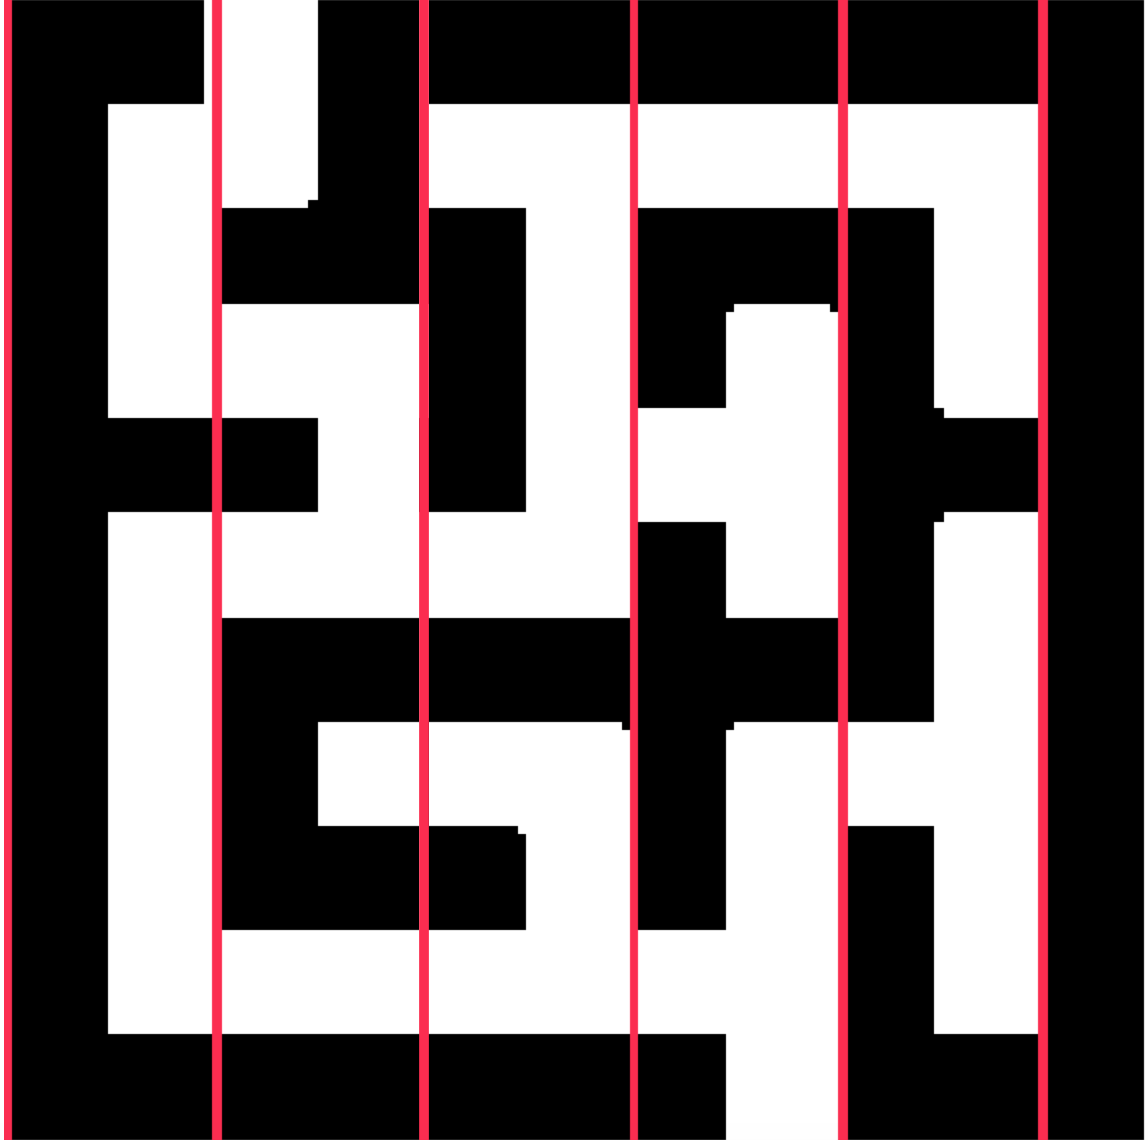
\includegraphics[width=5cm]{wallsall.png}
  \caption{Left wall edges}
  \label{fig:dijk}
\end{figure}

Once all of the walls have been found, the threshold grid can be decomposed into a maze grid. This is a binary grid that represents each square on a rectilinear maze - a 0 representing path and a 1 representing wall. An example of a maze grid is shown below.

\begin{figure}[H]
  \centering
  \includegraphics[width=5cm]{mazegrid.png}
  \caption{Maze grid}
  \label{fig:dijk}
\end{figure}

In the threshold grid, each pixel was represented by a binary number. Here, the pixels are grouped together into the blocks that make up the maze. This makes searching through the maze far more efficient. In order to create this grid, the maze is split up into sections using the wall positions. These sections are shown below - with the two wall sets show in different colours. Left-walls are shown in red, and up-walls in blue.

\begin{figure}[H]
  \centering
  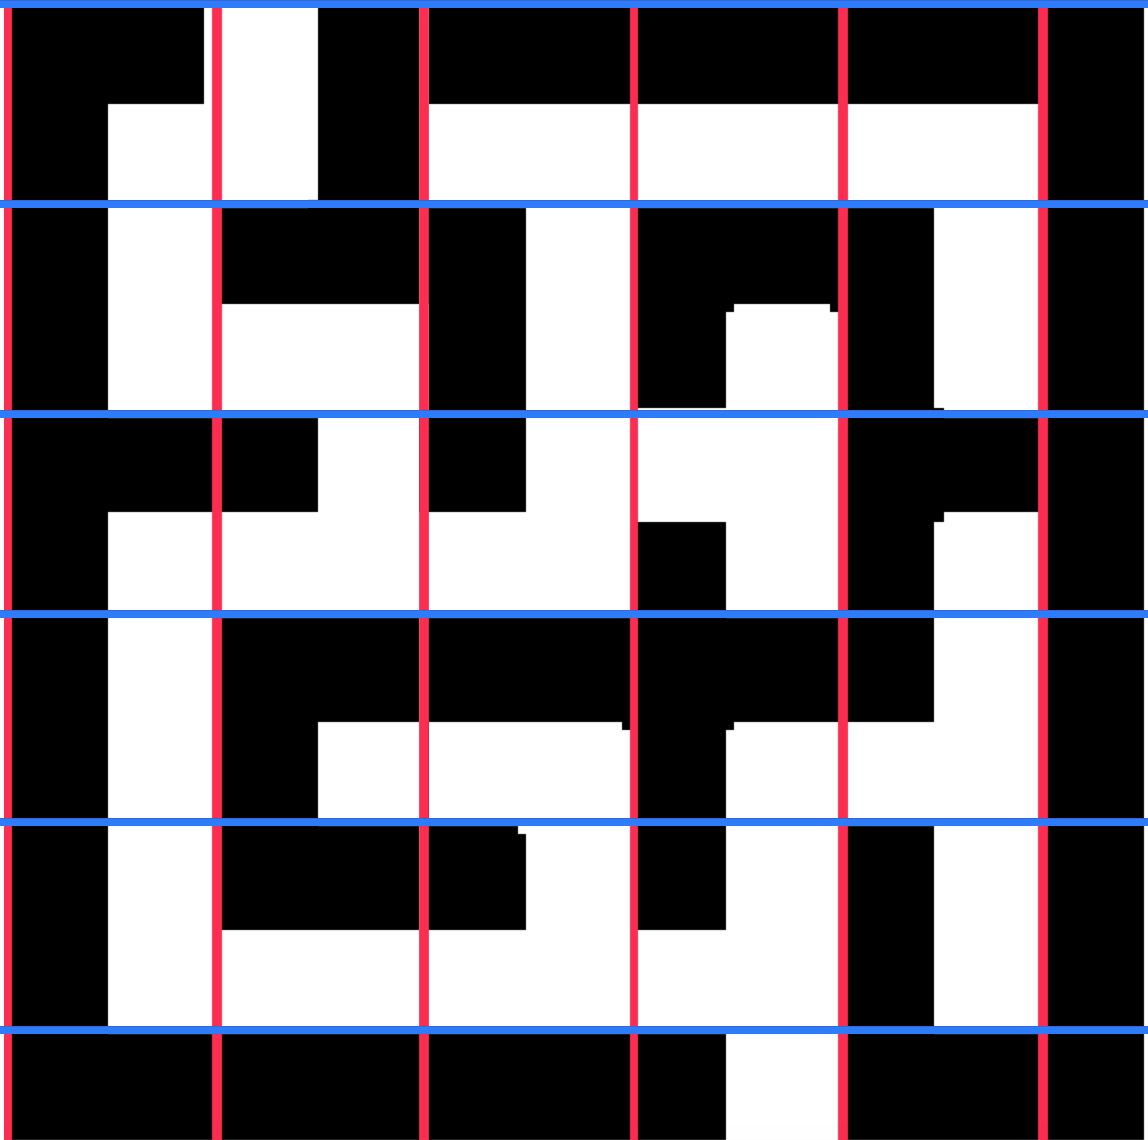
\includegraphics[width=5cm]{wallsmulti.png}
  \caption{Maze sections}
  \label{fig:dijk}
\end{figure}

Most of these sections contain 4 individual squares.  However, the final row and column sections only contain 2 squares each. This is because the number of walls is always one more than the number of paths that can run between them, as each path must be sandwiched between two walls. Therefore if there are m vertical walls and n horizontal walls, the maze grid will have dimensions 2m-1 x 2n-1. These location of each of these individual squares within a section is calculated using the average wall width and average wall height. In order to determine whether a square is wall or path, the density of the section is recorded using the threshold grid. If the density is greater than 0.25, it is a wall section. Otherwise, it is a path section. A pseudocode interpretation of this algorithm is shown below.

\begin{algorithm}[H]
\caption{Create Maze Grid}
\begin{algorithmic}[1]
    	\State wallsUp, wallsLeft $\gets$ \textbf{input}
    	\State mazeGrid $\gets$ [ ]
	\For {row \textbf{in} wallsUp}
		\For {col \textbf{in} wallsLeft}
			\For {sector \textbf{in} \textit{sectors}(row, col)}
				\If {\textit{density}(sector) $>$ 0.25}
					\State mazeGrid[sector] $\gets$ 1
	            	 	\Else
					\State mazeGrid[sector] $\gets$ 0
				\EndIf
			\EndFor
		\EndFor
	\EndFor
\end{algorithmic}
\end{algorithm}

I then prototyped this algorithm in R. 

\begin{changemargin}{-1in}{-1in} 
\begin{minted}[fontsize=\scriptsize]{r}
wall_widths <- sapply(walls_left, function(x) walls_right[walls_right>=x][1] - x)#AVERAGE DISTANCE BETWEEN SIDES OF WALL
wall_heights <- sapply(walls_up, function(x) walls_down[walls_down>=x][1] - x)
wall_width <- mean(wall_widths[wall_widths<=median(wall_widths)]) + 1           #ADD 1 DUE TO UNDERCALCULATION OF SIZE
wall_height <- mean(wall_heights[wall_heights<=median(wall_heights)]) + 1

maze_grid <- matrix(0, nrow=length(walls_up)*2-1, ncol=length(walls_left)*2-1)

for (y in 1:length(walls_up)) {                                                 #LOOP THROUGH SECTIONS
  for (x in 1:length(walls_left)) {
    top_left <- threshold_grid[walls_up[y]:(walls_up[y]+wall_height),           #CALCULATE DENSITY OF EACH SQUARE
                               walls_left[x]:(walls_left[x]+wall_width)]
    if (mean(top_left) > 0.25) {maze_grid[2*y-1, 2*x-1] <- 1}

    if (x < length(walls_left)) {
      top_right <- threshold_grid[walls_up[y]:(walls_up[y]+wall_height),
                                 (walls_left[x]+wall_width):walls_left[x+1]]
      if (mean(top_right) > 0.25) {maze_grid[2*y-1, 2*x] <- 1}
    }

    if (y < length(walls_up)) {
      bottom_left <- threshold_grid[(walls_up[y]+wall_height):walls_up[y+1],
                                    walls_left[x]:(walls_left[x]+wall_width)]
      if (mean(bottom_left) > 0.25) {maze_grid[2*y, 2*x-1] <- 1}
    }

    if (x < length(walls_left) && y < length(walls_up)) {
      bottom_right <- threshold_grid[(walls_up[y]+wall_height):walls_up[y+1],
                                     (walls_left[x]+wall_width):walls_left[x+1]]
      if (mean(bottom_right) > 0.25) {maze_grid[2*y, 2*x] <- 1}
    }
  }
}
\end{minted}
\end{changemargin} 

\subsubsection{Simplify Non-rectilinear Maze Image}

For mazes that are not rectilinear, this same level of analysis cannot be undertaken. Instead, a technique called Rectangular Symmetry Reduction, detailed in the analysis section, can be used. In order to implement this technique I used a new type of grid: the rect grid. This is a grid that represented each pixel of the image as either a 0, a 1 or a 2. A 0 in the rect grid represents a pixel that was not part of a rectangle. It could be either path or wall, but could not be placed within a larger rectangle. A 1 represents the perimeter of a square. It is always path, as the rectangles must be contained within empty space in the image. A 2 represents the inner section of the rectangle - the section that can be eliminated. In order for a rectangle to be any use it must have an inner section, so only rectangles with dimensions greater than 3x3 are considered. Such a grid is shown below, with the rectangles highlighted in red. 

\begin{figure}[H]
  \centering
  \includegraphics[width=5cm]{rectgrid.png}
  \caption{Rect grid}
  \label{fig:dijk}
\end{figure}

In order to create this rect grid, I needed to create an algorithm that could identify rectangles in the empty space of the binary grid. The algorithm would first calculate the maximum rectangle that could be drawn in empty space for each pixel, using the pixel as the foot of the rectangle (i.e. the pixel would be in the bottom-right corner of the rectangle. If a rectangle greater than 3x3 could be created, the dimensions of the rectangle was stored in a grid in the form m-n, where m is the width and n is the height of the rectangle. If a 3x3 rectangle was not possible, 0-0 is used instead. This grid was the area grid. It was the same size as the binary grid and rect grid, and represented the largest possible area of rectangle for each pixel. Look at the image below.

\begin{figure}[H]
  \centering
  \includegraphics[width=5cm]{abcrect.png}
  \caption{Rectangles within maze}
  \label{fig:dijk}
\end{figure}

For pixel A, the maximum size rectangle is 4x4. Therefore 4-4 is stored in this position in the area grid. For pixel B, only a 2x3 rectangle can be made, so 0-0 is stored - as rectangles must have a width and height of at least 3. For pixel C, the max rectangle is 5x3, so 5-3 is stored. Note that the first number represents width and the second height. Below this the full rect grid is shown with the A, B and C highlighted in red.

\begin{figure}[H]
  \centering
  \includegraphics[width=8cm]{areagrid.png}
  \caption{Area grid}
  \label{fig:dijk}
\end{figure}

To calculate the size of each rectangle, the algorithm scans left-wards to find a maximum area. It starts with a rectangle of width 1 and finds the maximum height this could be. It then increases the width until either the maximum height is less than 3, it hits the edge of the grid or hits a wall section. The height of the rectangle is determined by what is above it. As the width of the rectangle increases, this height can only decrease, as it is constrained by all of the obstacles above it (it can only encounter more obstacles, it cannot break free of the ones it has already found). Because of this, the algorithm keeps track of the current height, as well as the height and width of the rectangle that gave the maximum area. If the current height goes below three, it stops searching for rectangles - as all after this point will be useless. Look at the figure below.

\begin{figure}[H]
  \centering
  \includegraphics[width=8cm]{rectsteps.png}
  \caption{Finding the maximum area}
  \label{fig:dijk}
\end{figure}

In part 1, the current width of the rectangle is 1, and the current height is 5. The max width and max height are both initialised as 0 - as no valid rectangle has been found so far. In part 2 the width is increased to 2. Because the height above this pixel is 4, the current height is reduced to 4. No valid rectangle has been found, as the width is less than 3, so max width and max height remain at 0. In part 3 the width is incremented again. Although the height above this pixel is 5 again, the height of the rectangle is constrained to 4. However, this rectangle is valid - as the height and width are both at least 3. Therefore the max width is updated to 3 and the max height to 4. In part 4 the width is incremented again. Now the current height is less than 3 so the algorithm terminates for this pixel. A pseudocode interpretation of this algorithm is shown below.

\begin{algorithm}[H]
\caption{Create Area Grid}
\begin{algorithmic}[1]
    	\State binaryGrid $\gets$ \textbf{input}
    	\State areaGrid $\gets$ [ ]
   	\For {pixel \textbf{in} binaryGrid}
		\State width $\gets$ 1
		\State height $\gets$ \textit{heightAbove}(pixel)
		\State maxWidth, maxHeight $\gets$ 0
		\While {pixel.x - width $>$ 0 \textbf{and} height $>$ 2}
			\State bottomLeftPixel $\gets$ \textit{pixelAtPos}(pixel.x - width, pixel.y)
			\If {\textit{heightAbove}(bottomLeftPixel) $<$ height}
            			\State height $\gets$ \textit{heightAbove}(bottomLeftPixel)
			\EndIf
			\If {width $>$ 2 \textbf{and} height $>$ 2}
				\If {width $\times$ height $>$ maxWidth $\times$ maxHeight $>$}
					\State maxWidth $\gets$ width
					\State maxHeight $\gets$ height
				\EndIf
			\EndIf
			\State width $\gets$ width + 1
           	\EndWhile
		\State areaGrid[pixel.pos] $\gets$ [maxWidth, maxHeight]
        \EndFor
\end{algorithmic}
\end{algorithm}

I then implemented this algorithm in R. 

\begin{changemargin}{-1in}{-1in} 
\begin{minted}[fontsize=\scriptsize]{r}
height_above <- function(x, y) {                                                #FIND AMOUNT OF EMPTY SPACE ABOVE A CELL
  height <- 0
  while (threshold_grid[y-height, x] == 0 && y-height >= 1) {height <- height + 1}
  return(height)
}

max_area <- function(x, y) {                                                    #FIND LARGEST RECTANGLE FOR A GIVEN CELL
  width <- 1
  height <- height_above(x, y)
  max_width <- 0
  max_height <- 0
  while (height >= 3 && x - width >= 0) {                                       #LOOP THROUGH DIFFERENT WIDTHS
    if (height_above(x - (width-1), y) < height) {
      height <- height_above(x - (width-1), y)
    }
    if (width*height > max_width*max_height && width >= 3 && height >= 3) {     #NEW MAX RECT FOUND
      max_width <- width
      max_height <- height
    }
    width <- width + 1
  }
  return(paste(max_width, max_height, sep='-'))
}

area_grid <- matrix(mapply(max_area, col(threshold_grid), row(threshold_grid)), nrow=nrow(threshold_grid))
\end{minted}
\end{changemargin} 

I then printed the matrix area\_grid. As you can see, it is identical to the one in an earlier image.

\begin{figure}[H]
  \centering
  \includegraphics[width=12cm]{areaoutput.png}
  \caption{Area grid output}
  \label{fig:dijk}
\end{figure}

Once these maximum areas have been found, the algorithm then collates all of the details about each rectangle into a list (or vector, in R). Each item contains the x and y positions of the cell in the grid as well as the width and height of the rectangle, in the form x-y-width-height. It sorts this vector by area, so the largest rectangles are added first. This vector is sorted using a merge sort, which is detailed later on in the algorithms section. The rectangles with dimensions 0x0 are not added to this vector, they are simply ignored. 

Once sorted, each rectangle can be added to the rect grid. The exact steps the algorithm takes are as follows. First, it pops the first rectangle off the top of the sorted vector - which acts the same as a priority queue does. It then checks the bottom-right position of the rectangle (the position of the pixel it was created from) in the rect grid, to see that it is not part of another rectangle. If the value at this location is a 1 or a 2, there is already a rectangle there so the algorithm dumps this rectangle and pops the next one off the vector. If there is a 0, it is not part of another rectangle, so can be added to the rect grid. 

However, there is a lot of overlap between the rectangles, so they need to be trimmed before they are added. This is why the largest rectangles are added first: so that they can remove the most area without being trimmed needlessly. This trimming works by checking the top-most row and left-most column to see if they contain other rectangles. If the top-most row contains a part of another rectangle, the height of the current rectangle is reduced by one (trimming this row off the top of the rectangle). If the left-most column contains part of a rectangle, the width of the current rectangle is reduced by one. This is repeated until both the top row and top column are free from intersections, or until the rectangle is trimmed too far (the width or height become less than 3). Because of how these rectangles are created, the only parts of the rectangle that need to be trimmed are the top row and top column. This can be shown using the following diagram.

\begin{figure}[H]
  \centering
  \includegraphics[width=5cm]{overlap.png}
  \caption{Intersecting rectangles}
  \label{fig:dijk}
\end{figure}

Because we know the bottom-right corner does not overlap, if another rectangle (purple) overlaps the current rectangle (red) without overlapping the top row or left column then it must exist in one of the three states shown above. Because the rectangles with the largest areas are dealt with first, state 1 is impossible: the area of the purple rectangle is smaller so it cannot have been placed there first. State 2 is not possible for a different reason. Because the rectangles are all trying to occupy the max area, there would be no reason for the rectangle to stop half-way through the other rectangle, as the empty space continues left-wards. The area would be larger if it continued out to the left-hand column. Therefore, this state is also impossible. State 3 is not possible for the same reason.

A pseudocode interpretation of this algorithm is detailed below.

\begin{algorithm}[H]
\caption{Create Area Grid}
\begin{algorithmic}[1]
    	\State rectangleVector $\gets$ \textbf{input}
    	\State rectGrid $\gets$ [ ]
   	\For {rect \textbf{in} rectangleVector}
		\If {rectGrid[rect.bottomRight] $=$ 0}		
			\While {1 \textbf{or} 2 \textbf{in} rectGrid[rect.topRow] \textbf{and} rect.height $>$ 2}
				\State rect.height $\gets$ rect.height - 1
			\EndWhile
			\While {1 \textbf{or} 2 \textbf{in} rectGrid[rect.leftCol] \textbf{and} rect.width $>$ 2}
				\State rect.width $\gets$ rect.width - 1
			\EndWhile
			rectGrid[rect.area] $\gets$ 2
			rectGrid[rect.perimeter] $\gets$ 1
		\EndIf
        \EndFor
\end{algorithmic}
\end{algorithm}

I then prototyped this algorithm in R. I used a function called merge\_sort, which orders the rectangle data based on area. How it works is detailed in a later section - the algorithm is not very relevant in the section. It is listed under merge sort. 

\begin{changemargin}{-1in}{-1in} 
\begin{minted}[fontsize=\scriptsize]{python}
area_vector <- c()
for (y in 1:nrow(area_grid)) {
  for (x in 1:ncol(area_grid)) {
    data <- as.integer(strsplit(area_grid[y, x], '-')[[1]])
    area <- data[1] * data[2]
    if (area > 0) {
      area_vector <- c(area_vector, paste(x, y, data[1], data[2], sep='-'))
    }
  }
}

if (length(area_vector) > 0) {
  area_vector <- merge_sort(na.omit(area_vector), TRUE)
}

rect_grid <- matrix(0, nrow=nrow(area_grid), ncol=ncol(area_grid))
for (row in area_vector) {
  area_data <- as.integer(strsplit(row, '-')[[1]])
  x <- area_data[1]
  y <- area_data[2]
  width <- area_data[3]
  height <- area_data[4]
  if (rect_grid[y, x] == 0) {
    empty_row <- FALSE
    empty_col <- FALSE
    while (width >= 3 && height >= 3 && (!empty_row || !empty_col)) {
      if (!empty_row) {
        if (all(rect_grid[y-(height-1), (x-(width-1)):x] == 0)) {empty_row = TRUE}
        else {height <- height - 1}
      }
      if (!empty_col) {
        if (all(rect_grid[(y-(height-1)):y, x-(width-1)] == 0)) {empty_col = TRUE}
        else {width <- width - 1}
      }
    }
    if (width >= 3 && height >= 3) {
      rect_grid[(y-(height-1)):y, (x-(width-1)):x] <- 1
      rect_grid[(y-(height-1)+1):(y-1), (x-(width-1)+1):(x-1)] <- 2
    }
  }
}
\end{minted}
\end{changemargin} 

\subsubsection{Draw/Edit Maze}
As well as being loaded via an image, mazes can also be drawn from scratch, or edited once analysed. These are both done via the same program, as drawing a new maze is simply the same as editing an empty maze. If they are drawing a new maze from scratch, the user specifies the width and height of the maze and a blank image with these dimensions is created. This is then analysed to create an empty maze grid (one filled with 0s). The maze grid (which is empty if drawing or contains the maze if editing) is given as input to the drawing software. A new window is opened up in Processing that takes in the maze grid, along with the relative width and height of walls (these are set to 0.5 if drawing from scratch) and draws the maze to the screen. This relative width is the fraction of a cell that is taken up by wall - if wall and path cells are just as thick, the relative thickness is 0.5. The thicker the walls are relative to the empty path space between, the larger this value. In the maze grid, walls occur when the column or row number is odd, as they trap in path rows/columns. A path can only exist between two walls, as shown earlier in the design section. This means that the thickness of odd rows/columns is different to the thickness of even rows/columns. This is how the program represents the maze accurately. The program will use a function called dimensions to calculate where and how it should place a rectangle based on the index.

\begin{algorithm}[H]
\caption{Get Dimensions from Index}
\begin{algorithmic}[1]
    	\State cellSize, wallRatio $\gets$ \textbf{input}
    	\State indexX, indexY $\gets$ \textbf{input}
	\If {x.odd}
		\State rectX $\gets$ indexX $\div$ 2 $\times$ cellSize
		\State rectWidth $\gets$ wallRatio $\times$ cellSize
	\Else
		\State rectX $\gets$ (indexX $\div$ 2 + wallRatio) $\times$ cellSize
		\State rectWidth $\gets$ (1 - wallRatio) $\times$ cellSize
	\EndIf
	\If {y.odd}
		\State rectY $\gets$ indexY $\div$ 2 $\times$ cellSize
		\State rectHeight $\gets$ wallRatio $\times$ cellSize
	\Else
		\State rectY $\gets$ (indexY $\div$ 2 + wallRatio) $\times$ cellSize
		\State rectHeight $\gets$ (1 - wallRatio) $\times$ cellSize
	\EndIf
\end{algorithmic}
\end{algorithm}

When the user clicks on a cell, the value in the maze grid at that point is switched from 0 to 1, or 1 to 0. This change is then displayed to the user. If they click and drag, multiple cells are switched. However, the state is only changed once - if they click and hold on one point the state should not be switched repeatedly. This is done by keeping track of the last cell that has been selected whilst the mouse is pressed down. Only if the last cell is different to the current cell does the state of it change. This is shown in the pseudocode below.

\begin{algorithm}[H]
\caption{Edit Cells on Maze Grid}
\begin{algorithmic}[1]
	\State mouse $\gets$ \textbf{input}
	\State cell $\gets$ \textbf{input}
	\State prevCell $\gets$ \textbf{input}
	\If {mouse.clicked}
		\State cell.value $\gets$ 1 - cell.value
	\ElsIf {mouse.held \textbf{and} cell $\neq$ prevCell}
		\State cell.value $\gets$ 1 - cell.value
		\State prevCell $\gets$ cell
	\EndIf
\end{algorithmic}
\end{algorithm}

The program will also allow zooming and panning, to ensure that they can edit the minor details of the maze. These will be done via the keys. There will be three variables to keep track of: scale, xPan and yPan. These determine where the maze will be drawn using Processing's inbuilt translate and scale functions. The program will only allow a scale greater than about 0.9 (so there is a small border around the entire maze when completely zoomed out) and will only allow panning so that the maze is not dragged off the side of the window. 

Once the user has finished editing, they will press 's' and the new maze grid will be returned to the main program via a CSV file.

\subsubsection{Find Start and End Points}

Once the maze has been analysed, edited or drawn, it is ready to be solved. The user must select where they would like to solve the maze between. To do this, they can either use the auto-select algorithm, or click two points for themselves. The auto-select program iterates around the perimeter of the maze to find gaps, and places the end points here. Once two end points have been found it breaks. A pseudocode interpretation of this algorithm is shown below. 

\begin{algorithm}[H]
\caption{Auto-select End Points}
\begin{algorithmic}[1]
    	\State mazeGrid $\gets$ \textbf{input}
    	\State startPoint, endPoint $\gets$ \textbf{none}
	\For {cell \textbf{in} mazeGrid.perimeter}
		\If {cell.isWall}
			\If {startPoint.empty}
				\State startPoint $\gets$ cell
			\Else
				\State endPoint $\gets$ cell
				\State \textbf{break}
			\EndIf
		\EndIf
	\EndFor
\end{algorithmic}
\end{algorithm}

I prototyped this algorithm in Python, and tested it on a 5x5 grid.

\begin{changemargin}{-1in}{-1in} 
\begin{minted}[fontsize=\scriptsize]{python}
def auto_end_points(grid):                                                      #RETURN COORDINATES OF END POINTS
    start_point = None
    end_point = None
    found = False
    for x in range(len(grid[0])):                                               #LOOP THROUGH TOP ROW
        if found : break
        if grid[0][x] == 0:
            if start_point == None:
                start_point = [x, 0]
            else:
                end_point = [x, 0]
                found = True
    for x in range(len(grid[len(grid)-1])):                                     #LOOP THROUGH BOTTOM ROW
        if found : break
        if grid[len(grid)-1][x] == 0:
            if start_point == None:
                start_point = [x, len(grid)-1]
            else:
                end_point = [x, len(grid)-1]
                found = True
    for y in range(1, len(grid)-1):                                             #LOOP THROUGH LEFT COL
        if found : break
        if grid[y][0] == 0:
            if start_point == None:
                start_point = [0, y]
            else:
                end_point = [0, y]
                found = True
    for y in range(1, len(grid)-1):                                             #LOOP THROUGH RIGHT COL
        if found : break
        if grid[y][len(grid[0])-1] == 0:
            if start_point == None:
                start_point = [len(grid[0])-1, y]
            else:
                end_point = [len(grid[0])-1, y]
                found = True
    if end_point == None:
        return None
    return [start_point, end_point]

grid = [[1,0,1,1,1],                                                               #TEST GRID
[1,0,0,0,1],
[1,0,1,0,1],
[1,0,0,0,1],
[1,1,1,0,1]]

print(auto_end_points(grid))                       
\end{minted}
\end{changemargin} 

The program output [[1, 0], [3, 4]], which were the correct points.

The user can also select the points themselves. In this case, they can click to select points and press 's' to save their choices and return. If they select a third point, the first is removed and replaced with the new one. A pseudocode interpretation of this is shown below.

\begin{algorithm}[H]
\caption{Select End Points}
\begin{algorithmic}[1]
    	\State mazeGrid $\gets$ \textbf{input}
    	\State startPoint, endPoint $\gets$ \textbf{none}
	\State key $\gets$ \textbf{input}
	\While {key \textbf{not} s}
		\State key $\gets$ \textbf{input}
		\State cell $\gets$ \textbf{input}
		\If {cell.isPath}
			\If {startPoint.empty}
				\State startPoint $\gets$ cell
			\ElsIf {endPoint.empty}
				\State endPoint $\gets$ cell
			\Else
				\State startPoint $\gets$ endPoint
				\State endPoint $\gets$ cell
			\EndIf
		\EndIf
	\EndWhile
\end{algorithmic}
\end{algorithm}

I didn't prototype this section as it seemed incredibly simple to understand.

\subsubsection{Represent Maze Structure as Graph}

Once the maze has been analysed, it can be converted into a graph. This is done differently for rectilinear and non-rectilinear mazes. For rectilinear mazes, the maze grid is analysed and every junction or corner is made into a node, with edges drawn on to represent the paths between them. The weight of the edge represents the distance between the points. The start point and end point are also created as nodes, regardless of where they are. Dead ends are not added to the graph. This is because you cannot go anywhere from these dead ends: there would be no point adding them.  This can be seen in the image below.

\begin{figure}[H]
  \centering
  \includegraphics[width=8cm]{nbrs.png}
  \caption{Graph from maze}
  \label{fig:dijk}
\end{figure}

Red shows a cell with two neighbours: right and down. Neighbours are path cells directly (not diagonally) next to a cell. Because these two neighbours are not opposite one another (up and down or left and right), this cell is considered a corner (the path changes direction) so is modelled as a node. Purple, on the other hand, is not modelled as a node as the two neighbours are opposite one another. Yellow shows a junction: it has three neighbours. It is modelled as a node. Green is also a junction, this time with 4 neighbours. Pink only has two neighbours and isn't a corner, but it is the start point so is modelled as a node. Blue only has one neighbour. It is therefore a dead end and not modelled as a node. An pseudocode algorithm to check if a cell is a node or not is shown below

\begin{algorithm}[H]
\caption{Check if Cell is Valid Node}
\begin{algorithmic}[1]
    	\State cell $\gets$ \textbf{input}
    	\State endPoints $\gets$ \textbf{input}
    	\State nbrs $\gets$ cell.neighbours
	\If {cell.isWall}
		\State \Return \textbf{false}
	\ElsIf {cell \textbf{in} endPoints}
		\State \Return \textbf{true}
	\ElsIf {nbrs.amount $>$ 2}
		\State \Return \textbf{true}
	\ElsIf {nbrs.amount $<$ 2}
		\State \Return \textbf{false}
	\ElsIf{nbrs.opposite}
		\State \Return \textbf{false}
	\EndIf
	\State \Return \textbf{true}
\end{algorithmic}
\end{algorithm}

I then prototyped this algorithm in Python. I tested it on a 3x3 grid with two end points and have shown the code and results below

\begin{changemargin}{-1in}{-1in} 
\begin{minted}[fontsize=\scriptsize]{python}
def valid_node(x, y, grid, end_points):                                         #RETURNS TRUE/FALSE IS CELL IS NODE OR NOT
    if grid[y][x] == 1 : return False                                           #CELL IS WALL
    if [x,y] in end_points : return True
    nbrs_h = 0                                                                  #COUNT NUMBER OF HORIZONTAL/VERTICAL NBRS
    nbrs_v = 0
    if x > 0 : nbrs_h += 1 - grid[y][x-1]
    if y > 0 : nbrs_v += 1 - grid[y-1][x]
    if x < len(grid[y])-1 : nbrs_h += 1 - grid[y][x+1]
    if y < len(grid)-1 : nbrs_v += 1 - grid[y+1][x]
    if nbrs_h + nbrs_v > 2 : return True                                        #CELL IS JUNCTION
    if nbrs_h == 1 and nbrs_v == 1 : return True                                #CELL IS CORNER
    return False
    
g = [[1,1,0],                                                                   #TEST GRID
     [0,0,0],
     [0,1,0]]
ep = [[0,2], [2,2]]                                                             #TEST END POINTS
for y in range(3):  
    for x in range(3):
        print(x, y, valid_node(x, y, g, ep))
\end{minted}
\end{changemargin} 

\begin{figure}[H]
  \centering
  \includegraphics[width=5cm]{nbrout.png}
  \caption{Output}
  \label{fig:dijk}
\end{figure}

As you can see, it outputted every node correctly.

If the maze is non-rectilinear, the valid\_node function is implemented differently. Instead of checking to see whether or not a particular cell is node or not, it uses the rect grid to see if the cell has been eliminated by RSR. The first thing it does is check whether the cell is wall or not. If it is wall, it returns false immediately. If it isn't, it then checks to see if it is an end point, and returns true if it is. If it isn't, it then checks the rect grid. If a 2 is stored in its position, the algorithm returns false. If not, it returns true. Nodes are path cells that are either not eliminated by RSR or are end points. This is shown in the pseudocode below.

\begin{algorithm}[H]
\caption{Check if Cell is Valid Node}
\begin{algorithmic}[1]
    	\State cell $\gets$ \textbf{input}
    	\State endPoints $\gets$ \textbf{input}
    	\State rectGrid $\gets$ \textbf{input}
	\If {cell.isWall}
		\State \Return \textbf{false}
	\ElsIf {cell \textbf{in} endPoints}
		\State \Return \textbf{true}
	\ElsIf {rectGrid[cell.pos] $=$ 2}
		\State \Return \textbf{false}
	\EndIf
	\State \Return \textbf{false}
\end{algorithmic}
\end{algorithm}

This algorithm was very similar to the one before, so I didn't feel it would be beneficial to prototype this part as well. This was the only part that was different for rectilinear and non-rectilinear mazes: from now on the algorithms apply to both types (within this section, at least)

The program then loops through every cell in the grid to find the nodes. If the current cell is a valid node, it then searches upwards and left-wards to find the nodes it should be connected to. It searches until it finds either a valid node or a wall. The program returns a list of valid nodes, and the nodes they are connected to. A pseudocode interpretation of this algorithm is shown below. 

\begin{algorithm}[H]
\caption{Find Nodes in Maze Grid}
\begin{algorithmic}[1]
    	\State mazeGrid $\gets$ \textbf{input}
    	\State nodes $\gets$ [ ]
	\For {cell \textbf{in} mazeGrid}
		\If {\textit{validNode}(cell)}
			\State node $\gets$ cell
			\For {s \textbf{in} x \textbf{to} 1}
				\If {\textit{validNode}(mazeGrid[s, y])}
					\State node.nbrLeft $\gets$ s
					\State \textbf{break}
				\ElsIf {mazeGrid[s, y].isWall}
					\State \textbf{break}
				\EndIf
			\EndFor
			\For {s \textbf{in} y \textbf{to} 1}
				\If {\textit{validNode}(mazeGrid[x, s])}
					\State node.nbrUp $\gets$ s
					\State \textbf{break}
				\ElsIf {mazeGrid[x, s].isWall}
					\State \textbf{break}
				\EndIf
			\EndFor
			\State \textbf{append} node \textbf{to} nodes
		\EndIf
	\EndFor
\end{algorithmic}
\end{algorithm}

I then prototyped this algorithm in Python. I tested it on a 5x5 grid, which I have also displayed below. The image shows where the nodes should be in green, and the output displays the node's x coordinate, y coordinate, left-neighbours x coordinate and up-neighbours y coordinate. The reason the neighbours only need one coordinate is that they are on the same row/column as the node so only the other coordinate is needed. The start and end points are also displayed, in blue. 

\begin{changemargin}{-1in}{-1in} 
\begin{minted}[fontsize=\scriptsize]{python}
def get_nodes(grid, end_points):                                                #RETURNS LIST OF NODE POS AND NBR POS
    nodes = []
    for y in range(len(grid)):
        for x in range(len(grid[y])):
            if valid_node(x, y, grid, end_points):
                nbr_left = -1
                nbr_up = -1
                for s in range(x-1, -1, -1):                                    #FIND NBR TO LEFT
                    if valid_node(s, y, grid, end_points):
                        nbr_left = s
                        break
                    elif grid[y][s] == 1:
                        break
                for s in range(y-1, -1, -1):                                    #FIND NBR ABOVE
                    if valid_node(x, s, grid, end_points):
                        nbr_up = s
                        break
                    elif grid[s][x] == 1:
                        break
                nodes.append([x, y, nbr_left, nbr_up])
    return nodes

g = [[1,0,1,1,0],                                                               #TEST GRID
     [0,0,0,0,0],
     [0,1,0,1,1],
     [0,1,0,1,0],
     [0,0,0,0,0]]
ep = [[0,2], [2,2]]                                                             #TEST END POINTS
nodes = get_nodes(g, ep)
for n in nodes:
    print(n)
\end{minted}
\end{changemargin} 

\begin{figure}[!htb]
\minipage{0.5\textwidth}
  \includegraphics[width=\linewidth]{greenode.png}
  \caption{Input grid}\label{fig:euc}
\endminipage\hfill
\minipage{0.5\textwidth}
  \includegraphics[width=\linewidth]{nodenbr.png}
  \caption{Output}\label{fig:manhat}
\endminipage\hfill
\end{figure}

As you can see, it worked perfectly. The correct nodes with the correct neighbours have been placed together.

Now this list of details needs to be converted into a more accessible format for storing a graph - namely either an adjacency matrix or an adjacency list. Because each node only has a very few number of neighbours (maximum 4) relative to the total number of nodes (which could range from 10 to 10000+), I chose to use an adjacency list. I will store my adjacency list as a hash table, which allowed for rapid lookup of my nodes in $O(1)$ time. I have written more about the hash table I will use in the data structures section, as it is more relevant there. For the prototyping after the pseudocode I will use Python's in-built dictionary class, but I plan to implement my own hash table for the actual program. The program converts this list into a dictionary by looping through each item and creating an ID for the node, in the form 'x-y'. This is the key for the dictionary. It then creates IDs for the neighbours, and sets a list of these IDs as the value for the key. It then uses these keys to add the node to the list of each of the neighbours, so that they are linked both ways. This can be shown in the pseudocode below. 

\begin{algorithm}[H]
\caption{Create Adjacency Dictionary}
\begin{algorithmic}[1]
    	\State nodeList $\gets$ \textbf{input}
    	\State adjacencyList $\gets$ \{ \}
	\For {node \textbf{in} nodeList}
		\State id $\gets$ node[0] + '-' + node[1]
		\State adjacencyList[id] $\gets$ [ ]
		\If {node[2] $>=$ 0}
			\State idLeft $\gets$ node[2] + '-' + node[1]
			\State \textbf{append} idLeft \textbf{to} adjacencyList[id]
			\State \textbf{append} id \textbf{to} adjacencyList[idLeft]
		\EndIf
		\If {node[3] $>=$ 0}
			\State idUp $\gets$ node[0] + '-' + node[3]
			\State \textbf{append} idUp \textbf{to} adjacencyList[id]
			\State \textbf{append} id \textbf{to} adjacencyList[idUp]
		\EndIf
	\EndFor
\end{algorithmic}
\end{algorithm}

I then prototyped the algorithm in Python. I included a section to test the function on the same grid as before and print the results in the form "nodeID [nbrID]". The output is displayed below. 

\begin{changemargin}{-1in}{-1in} 
\begin{minted}[fontsize=\scriptsize]{python}
def adjacency_dict(nodes_list):                                                 #RETURNS DICTIONARY OF ADJACENCIES
    adj_dict = {}
    for node_data in nodes_list:
        node_id = str(node_data[0]) + '-' + str(node_data[1])
        adj_dict[node_id] = []  
        if node_data[2] >= 0:                                                   #IF ADJACENCY EXISTS
            left_id = str(node_data[2]) + '-' + str(node_data[1])
            adj_dict[node_id].append(left_id)                                   #ADD ADJACENCY BOTH WAYS
            adj_dict[left_id].append(node_id)
        if node_data[3] >= 0:
            up_id = str(node_data[0]) + '-' + str(node_data[3])
            adj_dict[node_id].append(up_id)
            adj_dict[up_id].append(node_id)
    return adj_dict

g = [[1,0,1,1,0],                                                               #TEST GRID
     [0,0,0,0,0],
     [0,1,0,1,1],
     [0,1,0,1,0],
     [0,0,0,0,0]]
ep = [[0,2], [2,2]]                                                             #TEST END POINTS
nodes_list = get_nodes(g, ep)
adj_dict = adjacency_dict(nodes_list)
for key in adj_dict.keys():
    print(key, adj_dict[key])
\end{minted}
\end{changemargin} 

\begin{figure}[H]
  \centering
  \includegraphics[width=5cm]{adjout.png}
  \caption{Output}
  \label{fig:dijk}
\end{figure}

\subsubsection{Solve Maze}
Once it has been converted into a graph, the maze can then be solved. It is solved using A*, an algorithm that was described extensively in the research section. Below is a pseudocode interpretation of it.

\begin{algorithm}
\caption{A* Algorithm}
\begin{algorithmic}[1]
	\State start, end $\gets$ \textbf{input}
  	\State queue $\gets$ [start]
	\State visited $\gets$ [ ]
	\State visiting $\gets$ \textbf{none}
	\While {visiting $\neq$ end}
    		\State visiting $\gets$ queue[0]
        		\For {adjacent \textbf{in} visiting.adjacents}
		        \State score $\gets$ $g($adjacent$) + h($adjacent$)$
        			\If {adjacent \textbf{not in} visited}
				\State adjacent.score $\gets$ score
				\State adjacent.previous $\gets$ visiting
                			\State \textbf{append} adjacent \textbf{to} visited
			\ElsIf {score < adjacent.score}
				\State adjacent.score $\gets$ score
				\State adjacent.previous $\gets$ visiting
                			\State \textbf{update} adjacent \textbf{in} visited
			\EndIf
    		\EndFor
    	\EndWhile
\end{algorithmic}
\end{algorithm}

Once the end node has been found, the path is created by looping back through each node's previous node until the start is reached. This is shown in the pseudocode below. 

\begin{algorithm}
\caption{Get Path}
\begin{algorithmic}[1]
	\State start, end $\gets$ \textbf{input}
	\State path $\gets$ [ ]
	\State \textbf{append} end \textbf{to} path 
	\State current $\gets$ end
	\While {current $\neq$ start}
		\State \textbf{append} current \textbf{to} path 
		\State current $\gets$ current.previous
	\EndWhile
	\State \textbf{append} start \textbf{to} path 
\end{algorithmic}
\end{algorithm}
		
\subsubsection{Merge Sort}
The merge sort is used in two places in the code: to sort the walls into the correct order (when the missed walls are added, they need to be sorted into the right order) and to sort the rectangle data by area. I chose to implement a merge sort, as it is able to sort the data in $O(n\log n)$. A pseudocode interpretation of the algorithm is shown below.

\begin{algorithm}[H]
\caption{Merge Sort}
\begin{algorithmic}[1]
	\Procedure{Merge}{a, b}
		\State c  $\gets$ [ ]
		\While {a.length $>$ 0 \textbf{and} b.length $>$ 0}
			\If {a[1] $>$ b[1]}
				\State \textbf{append} a[1] \textbf{to} c
			\Else
				\State \textbf{append} b[1] \textbf{to} c
			\EndIf
		\EndWhile
		\While {a.length $>$ 0}
			\State \textbf{append} a[1] \textbf{to} c
		\EndWhile
		\While {b.length $>$ 0}
			\State \textbf{append} b[1] \textbf{to} c
		\EndWhile
		\State \Return c
	\EndProcedure
	\State 
	\Procedure{MergeSort}{a}
		\If {a.length $=$ 1}
			\State \Return a
		\EndIf
		\State midpoint $\gets$ a.length $\div$ 2
		\State b $\gets$ a[1 \textbf{to} midpoint]
		\State c $\gets$ a[midpoint \textbf{to} a.length]
		\State \Return \Call{Merge}{b, c}
	\EndProcedure
\end{algorithmic}
\end{algorithm}

I then prototyped this algorithm in Python. This algorithm utilises a third function: value. It takes in an item and either returns it as is (if it is a wall position) or returns the negative product of the rectangle's dimensions (if it is data about a rectangle). It returns the negative product because the wall positions are ordered from smallest to largest, but the rectangles are ordered from largest to smallest. This allows the same function to be used for both data types and both orders, as a negative number with a large magnitude is less than a negative number with a small magnitude. 

\begin{changemargin}{-1in}{-1in} 
\begin{minted}[fontsize=\scriptsize]{python}
def merge(list_a, list_b, sort_areas):                                          #MERGES TWO LISTS TOGETHER
    pointer_a = 0
    pointer_b = 0
    merged = []

    while (pointer_a < len(list_a)) & (pointer_b < len(list_b)):                #WHILE BOTH LISTS NOT EMPTY
        if value(list_a[pointer_a], sort_areas) < value(list_b[pointer_b], sort_areas):
            merged.append(list_a[pointer_a])                                    #ADD FROM A IF SMALLER THAN B (OR MORE NEGATIVE)
            pointer_a += 1
        else:
            merged.append(list_b[pointer_b])
            pointer_b += 1

    if pointer_a < len(list_a):                                                 #ADD REMNANTS
        merged += list_a[pointer_a:]
    elif pointer_b < len(list_b):
        merged += list_b[pointer_b:]
    return merged

def sort(main_list, sort_areas = False):                                        #SORT LIST USING MERGE SORT
    list_a = main_list[:len(main_list)//2]
    list_b = main_list[len(main_list)//2:]
    if len(list_a) > 1:
        list_a = sort(list_a, sort_areas)
    if len(list_b) > 1:
        list_b = sort(list_b, sort_areas)
    return merge(list_a, list_b, sort_areas)   

def value(item, sort_areas):                                                    #RETURNS VALUE THAT ITEMS ARE ORDERED BY
    if sort_areas:
        data = item.split('-')
        return -int(data[2])*int(data[3])                                       #WANT TO ORDER BY LARGEST NOT SMALLEST SO MAKE NEGATIVE
    return item                                                                 #WANT TO ORDER BY SMALLEST SO LEAVE AS IS
\end{minted}
\end{changemargin} 


\subsection{Data Structures}
I used several different data structures in order to store different information. These are explained below, along with some algorithms that are directly and solely related to maintaining the structure.

\subsubsection{Min Heap}
In order to implement the A* algorithm I will need to use a priority queue to store nodes. I will do this via a min-heap, as it allows for both pushing and popping in $O(\log n)$. Through my implementation, I will also be able to update the position of an item in $O(\log n)$ and find an item in $O(1)$.

A min-heap is a type of binary tree that keeps smaller items closer to the root. It must obey two properties: the order property and the shape property. The order property states that a node must have a value smaller than or equal to values of its two children. The shape property states that (1) all leaves must be at a depth of d or d-1, (2) all leaves of depth d-1 are to the right of leaves with a depth of d, (3a) there is at most 1 node with only 1 child and (3b) that child must be the left-child of the node and (3c) it is the right-most leaf at depth d. These rules are visualised by the diagram below.

\begin{figure}[H]
  \centering
  \includegraphics[width=12cm]{maxheap.png}
  \caption{Min-heap properties}
  \label{fig:dijk}
\end{figure}

My min-heap must be able to add, remove and also update. The min-heap is stored as an array, with an empty item in index 0. This is to ensure indexing starts at 1, so that if a node is in array[k], its left child is in array[k*2] and the right in array[k*2 + 1]. If a node is in array[k], its parent is in array[k/2] by integer division. The process of adding a new item works as follows: first, the item is added to the end of the heap. It is then bubbled upwards. This is comparing the item to its parent, and swapping it while its value is smaller than its parent's value. A pseudocode interpretation of this is shown below.

\begin{algorithm}[H]
\caption{Min-heap Add}
\begin{algorithmic}[1]
	\Procedure{BubbleUp}{current}
	\State parent $\gets$ current $\div$ 2
	\While {parent $>=$ 1 \textbf{and} minHeap[current] $<$ minHeap[parent]}
		\State \textbf{swap} minHeap[current] \textbf{and} minHeap[parent]
		\State current $\gets$ parent
		\State parent $\gets$ current $\div$ 2
	\EndWhile
	\EndProcedure
	\State
	\Procedure{Add}{item}
		\State \textbf{append} item \textbf{to} minHeap
		\State pos $\gets$ minHeap.length
		\State \Call{BubbleUp}{pos}
	\EndProcedure
\end{algorithmic}
\end{algorithm}

Remove-min, or pop, is implemented in a similar way, using bubbling down instead. The items in the first index and last index are swapped, and the last item is then removed. Then, the root node is bubbled down by comparing the current node with its children and swapping it with the smallest child it is greater than. This is shown in the pseudocode below.

\begin{algorithm}[H]
\caption{Min-heap Remove}
\begin{algorithmic}[1]
	\Procedure{BubbleDown}{current}
		\State a $\gets$ current $\times$ 2
		\State b $\gets$ current $\times$ 2 $+$ 1
		\While {b $<=$ minHeap.length}
			\If {minHeap[a] $<=$ minHeap[b] $<=$  minHeap[current]}
				\State \textbf{swap} minHeap[current] \textbf{and} minHeap[b]
				\State current $\gets$ b
			\ElsIf {minHeap[b] $<=$ minHeap[a] $<=$  minHeap[current]}
				\State \textbf{swap} minHeap[current] \textbf{and} minHeap[a]
				\State current $\gets$ a
			\Else
				\State \textbf{break}
			\EndIf
			\State a $\gets$ current $\times$ 2
			\State b $\gets$ current $\times$ 2 $+$ 1
		\EndWhile
	\EndProcedure
	\State
	\Procedure{Remove}{}
		\State \textbf{swap} minHeap.head \textbf{and} minHeap.tail
		\State item $\gets$ minHeap.tail
		\State \textbf{remove} minHeap.tail
		\State pos $\gets$ 1
		\State \Call{BubbleDown}{pos}
		\State \Return item
	\EndProcedure
\end{algorithmic}
\end{algorithm}

I then looked at how I could implement update - which is needed when a node's score is changed. When this happens, it needs to move within the priority queue. Because each node is represented as an object, I could store its index in the queue as a property of the object, meaning finding the object within the queue took $O(1)$ time. I then simply bubbled the object, with its new value, up. Because of how A* works, a node's score would only ever reduce. Therefore the node should simply be bubbled upwards. This is shown by the very simple pseudocode below.

\begin{algorithm}[H]
\caption{Min-heap Update}
\begin{algorithmic}[1]
	\Procedure{Update}{pos}
		\State \Call{BubbleUp}{pos}
	\EndProcedure
\end{algorithmic}
\end{algorithm}

\subsubsection{Hash Table}
Another data structure used within the program is a hash table. It is used to represent both an adjacency list and a reference table to access node objects by their id. Both require the key to be an id in the form x-y, where x is the x-position of the node and y being the y-position. I therefore needed a hashing algorithm that could convert these into a index whilst minimising clustering (many keys mapping to one index). I chose to use Cormen's Multiplication Method, which works by taking a relatively random-looking number (one suggested was $0.5 \times \sqrt{5} - 1$) and multiplying by the number created from the key (created by removing the dash from the id). Then take the fractional part of the answer and multiply it by the capacity of the hash table. Flooring this number gives the index. This can be shown in the following pseudocode.

\begin{algorithm}[H]
\caption{Get Index for Hash Table}
\begin{algorithmic}[1]
	\Procedure{Index}{key}
		\State value $\gets$ key \textbf{without} '-' 
		\State product $\gets$ value $ \times 0.5 \times \sqrt{5} - 1$
		\State index $\gets$ \textbf{floor} hashTable.capacity $\times$ product
	\EndProcedure
\end{algorithmic}
\end{algorithm}

In order to deal with collisions, I will implement chaining. This works by storing each item inserted into the hash table in a two-dimensional list. Each of the lists within the list are in the form [key, item]. When finding the item by key, first the key is put through the hash function to determine the index. Then, the list stored at this index in the table is iterated through until the correct key is found via the [key, item] lists. I prototyped the algorithm in Python to show how the chaining will work.

\begin{changemargin}{-1in}{-1in} 
\begin{minted}[fontsize=\scriptsize]{python}
class Hash:                                                                     #HASH TABLE CLASS
    def __init__(self, size):
        self.size = size                                                        #SET CAPACITY
        self.table = []
        for i in self.size : self.table.append([])

    def index(self, key):                                                       #HASH FUNCTION
        value = int(key.replace('-',''))
        frac = value * 0.5 * (math.sqrt(5) - 1) % 1
        return math.floor(self.size * frac)
    
    def __setitem__(self, key, value):                                          #ADD ITEM TO TABLE
        index = self.index(key)
        items = self.data[index]
        items.append([key, value])

    def __getitem__(self, key):                                                 #GET ITEM BY KEY
        index = self.hash_function(key)
        items = self.data[index]
        for item in items:
            if item[0] == key : return item[1]
        return None
\end{minted}
\end{changemargin} 


\subsubsection{Specific Examples of Data Structures}
I have included a small paragraph about each of the other data structures used in the program. There is less to explain about these, so I have written less.

\textbf{Image to maze grid conversion}
\begin{quote}
\textbf{RGB grid} - this stores an $m \times n$ array of tuples, where m is the width of the image and n is the height so that each tuple represents a single pixel. The tuples contain three values each - in the form (R, G, B) where R is an integer that specifies red light intensity, G specifies green and B specifies blue.
\\\\
\textbf{Greyscale grid}  - this stores an $m \times n$ array of integers, where $m$ is the width of the image and $n$ is the height so that each integer represents a single pixel. Each integer represents the luminosity of a pixel (the greyscale value).
\\\\
\textbf{Luminance histogram} - this stores the frequency of every luminance value within the greyscale grid. It is a vector that represents the number of pixels in the image that have the specified luminance value, from 1 to the maximum luminance in the image.
\\\\
\textbf{Weighted histogram} - this is the luminance histogram multiplied by the actual luminance value, so that every item is calculated by luminance $\times$ frequency. It allows the means needed for Otsu's method to be calculated far more quickly.
\\\\
\textbf{Threshold grid} - this stores an $m \times n$ array of binary values (0 or 1), where $m$ is the width of the image and $n$ is the height so that each digit represents a single pixel. Pixels with a luminosity below a specific threshold are represented by a 0, and those with a luminosity above it are represented by a 1. If the maze is inverted, the opposite is true (0 = above, 1 = below).
\\\\
\textbf{Frequency vector} - this stores the frequency of wall pixels in the threshold grid per row or column. There are two vectors, one for rows (horizontal) and one for columns (vertical).
\\\\
\textbf{Edges vector} - this stores the difference in frequency between neighbouring rows/columns. There are four vectors: up-edges, down-edges, left-edges and right-edges. Each stores edges in the specified direction.
\\\\
\textbf{Central edges vector} - this stores horizontal/vertical edges in both directions (either both up-edges and down-edges or left-edges and right-edges), except the first and last edges. This is because these edges are often much larger than the others, as they represent the start and end of the maze. There are two vectors, one horizontal and one vertical, used to calculate the threshold value for which edges are considered to be walls.
\\\\
\textbf{Walls vector} - this stores the positions of rows/columns that have edge values great enough to be considered walls. There are four vectors: up-walls, down-walls, left-walls and right-walls.
\\\\
\textbf{Density grid} - this stores an $m \times n$ array of float values (0 to 1), where $m$ is the width of the maze and $n$ is the height so that each digit represents a single maze cell. The float value represents the fraction of the section that is wall (i.e. it represents the density of '1' values within a section).
\\\\
\textbf{Maze grid} - this stores an $m \times n$ array of binary values (0 or 1), where $m$ is the width of the maze and $n$ is the height so that each digit represents a single maze cell. A 0 represents a path section, and a 1 represents a wall section. A 0 is placed in sections with a low density, a 1 in sections with a high density.
\end{quote}

\textbf{Draw/edit maze}
\begin{quote}
\textbf{Keys array} - this is a boolean array that stores which of 8 specified keys are currently being pressed down. The keys are [up, down, left, right, z, x, y, cmd/ctrl].
\\\\
\textbf{Maze grid} - this functions the same as the maze grid detailed above.
\end{quote}

\textbf{Rectangular Symmetry Reduction}
\begin{quote}
\textbf{Height grid} - this stores an $m \times n$ array of integer values, where $m$ is the width of the image and $n$ is the height so that each digit represents a single pixel. This grid is used during RSR, so is only used with non-rectilinear mazes. Each integer represents the amount of empty space above a specific cell until the next wall. It is used to calculate maximum rectangle areas without lots of recalculations.
\\\\
\textbf{Area grid} - this stores an $m \times n$ array of string values, where $m$ is the width of the image and $n$ is the height so that each digit represents a single pixel. The string values are in the form 'w-h' where w is the width of the rectangle and h is the height. Each represents the maximum rectangle size that can be drawn, starting from that pixel.
\\\\
\textbf{Area vector} - this stores a sorted vector of string values. It is sorted by area, and each string is in the form 'x-y-w-h' where (x, y) is the position of the rectangle's bottom-right corner, w is the width and h the height.
\\\\
\textbf{Rect grid} - this stores an $m \times n$ array of integer values (0 to 2), where $m$ is the width of the image and $n$ is the height so that each digit represents a single pixel. The values represent whether or not a pixel is part of a rectangle A 0 means it is not, a 1 means it is on the perimeter and a 2 means it is enclosed within a rectangle (so can be ignored).
\end{quote}

\textbf{Select/auto-select end points}
\begin{quote}
\textbf{End points} - this is an array of length 4 that stores the co-ordinates of the start/end points of the route. It is in the form [sx, sy, ex, ey] where (sx, sy) is the position of the start point, and (ex, ey) is the position of the end point.
\end{quote}

\textbf{Convert maze to graph}
\begin{quote}
\textbf{Nodes grid} - this stores an $4 \times n$ array of integer values, where 4 is the width of the node grid and $n$ is the number of valid nodes. It is a grid with four columns, with each row representing a different node. The first column represents the x-position of the node, the second the y-position, the third the x-position of the left-neighbour (-1 if none) and the fourth the y-position of the right-neighbour (-1 if none).
\\\\
\textbf{Adjacency table} - this is a hash table that stores the neighbours of each node. It takes in a key in the form 'x-y' where (x, y) is the position of the node. It returns a list of neighbours, each in the same form.
\end{quote}

\textbf{Solve maze}
\begin{quote}
\textbf{Nodes table} - this is a hash table that acts as a look-up table for node objects by their ID. It allows the specific object for a node to be accessed by its ID in $O(1)$ instead of having to search for it.
\\\\
\textbf{Nodes queue} - this is a priority queue that orders the nodes to be explored by the A* algorithm. It orders them based on their score, with the lowest scoring nodes opened first. 
\end{quote}


\subsection{GUI Design}
The GUI will consist of one main Tkinter window and another smaller pop-up Processing window that is used for drawing/editing/selecting. The main window will feature a row of buttons along the top and a main canvas element over the rest of the window. The canvas is used for drawing the maze to the screen and displaying informational text. The buttons currently being displayed will changed based on what the user is currently doing.

\subsubsection{Finite State Model}
This main window exists in several different states, depending on what the user is doing. The different states can be modelled as an FSM, in order to explain how the user can travel between states. Each of the states is given a name, and the arrows between them represent a button being pressed. From every state the user can return to the main menu by pressing 'return to main menu', but these arrows have been left off the diagram as they would clutter it up too much and are self-explanatory. Some of the arrows say 'automatic when finished' - this means that the program will automatically progress to the next state once it has finished its processes in the current state.

\begin{figure}[H]
  \centering
  \includegraphics[width=12cm]{FSM.png}
  \caption{Finite state machine}
  \label{fig:dijk}
\end{figure}

Each of the following sections describes how the window will look in different states.

\subsubsection{Main Menu}
\begin{figure}[H]
  \centering
  \includegraphics[width=12cm]{Slide1.png}
  \caption{Main menu mockup}
  \label{fig:dijk}
\end{figure}
This window acts as the main menu. It allows the user to either load an image or draw an image. It is used when in 'main' state.
\begin{enumerate}
\item This button allows the user to load a maze from an image file. They will be asked to select the file via a file browser, and then the file will be opened and analysed.
\item This button allows the user to create a maze from scratch, using the drawing software. They will be asked to specify the width and height of the image in pixels, as well as a name for the maze. The design for the drawing software is detailed later.
\item This button is used to display helpful messages to the user. It will pop up a dialogue box that explains the purpose of every button currently on screen.
\item This is the canvas. It will either display helpful messages to the user or display the maze in its current state. For the main menu, it will display the message 'Load/draw maze to start'
\end{enumerate}

\subsubsection{Update Window}
\begin{figure}[H]
  \centering
  \includegraphics[width=12cm]{Slide2.png}
  \caption{Update window mockup}
  \label{fig:dijk}
\end{figure}
This window is used when a task is currently being threaded. It is used when in the states: 'creating', 'drawing', 'editing', 'selecting', and 'finding'.
\begin{enumerate}
\item This button allows the user to return to the main menu. It causes the threaded process to be quit.
\item This button is used to display helpful messages to the user. It will pop up a dialogue box that explains the purpose of every button currently on screen.
\item The canvas will display text messages from the update.txt file. It will read the file and display the contents on the screen. 
\end{enumerate}

\subsubsection{Image Window}
\begin{figure}[H]
  \centering
  \includegraphics[width=12cm]{Slide3.png}
  \caption{Image window mockup}
  \label{fig:dijk}
\end{figure}
This window is used during the 'image' state. It displays the analysed image to the screen.
\begin{enumerate}
\item This button is used to edit the maze. Pressing it opens up a Processing window used to edit the maze.
\item This button inverts the maze and reloads this window, swapping path and wall cells in the maze. 
\item This button auto-selects the end points for the user, using the algorithm detailed earlier.
\item This button opens up a Processing window that allows the user to select the end points themselves.
\item This button opens a window that displays the image on the canvas in a larger format. This is handled by the OS, so on a mac the image will be displayed by Preview.
\item This button allows the user to return to the main menu.
\item This button is used to display helpful messages to the user. It will pop up a dialogue box that explains the purpose of every button currently on screen.
\item This displays the maze grid to the screen once the image has been analysed. A 0 in the maze grid (path) is represented by a white square, with a 1 (wall) represented by a black square. 
\end{enumerate}

\subsubsection{End Points Window}
\begin{figure}[H]
  \centering
  \includegraphics[width=12cm]{Slide4.png}
  \caption{End points window mockup}
  \label{fig:dijk}
\end{figure}
This window is used during the 'points' state. It displays the end points and maze to the user.
\begin{enumerate}
\item This button allows the user to go back a stage, so that they can either select different end points or edit the maze. It goes back to the 'image' state.
\item This button opens a window that displays the image on the canvas in a larger format. 
\item This button causes the program to solve the maze between the two selected end points.
\item This button allows the user to return to the main menu.
\item This button is used to display helpful messages to the user. It will pop up a dialogue box that explains the purpose of every button currently on screen.
\item This displays the maze grid and end points to the user. The end points are displayed in red.
\end{enumerate}

\subsubsection{Solved Path Window}
\begin{figure}[H]
  \centering
  \includegraphics[width=12cm]{Slide5.png}
  \caption{Solved path window mockup}
  \label{fig:dijk}
\end{figure}
This window displays the solved maze to the user. It is used during the 'path' state.
\begin{enumerate}
\item This button allows the user to go back to the 'image' state, so that they can either select different end points or edit the maze.
\item This button saves the image currently displayed on the screen. It saves the maze in the form 'example-path.png' where 'example.png' was the original image.
\item This button is used to change the colour gradient used to draw the path. The default is blue to red, but the user can specify any two RGB colours. 
\item This button opens a window that displays the image on the canvas in a larger format. 
\item This button allows the user to return to the main menu.
\item This button is used to display helpful messages to the user. It will pop up a dialogue box that explains the purpose of every button currently on screen.
\item The image displayed on the screen is the original image with the path drawn over the top. If the maze has been edited or drawn from scratch, the original image is not used and a new maze image is created by using the maze grid, with a 1 being drawn as a black square and a 0 a white square.
\end{enumerate}

\subsubsection{Draw/Edit/Select Points Window}
\begin{figure}[H]
  \centering
  \includegraphics[width=12cm]{Slide6.png}
  \caption{Draw/Edit/Select [Processing] window mockup}
  \label{fig:dijk}
\end{figure}

This window will be used to edit mazes, draw mazes and select the end points. This window is separate to the Tkinter window. It is used during the 'drawing', 'selecting' and 'editing' states.
\begin{enumerate}
\item This is the main canvas. It will draw the maze onto the screen. The size and position of the maze depends on the zoom and the scale used selected by the user. Also, the width of the walls will reflect the width of the walls in the original image. If the original wall width is narrow, the displayed width will also be narrow.
\item This is the information window. It can be toggled on and off (hidden and displayed) using the 'h' key. It is slightly transparent so that the maze can be seen behind.
\end{enumerate}

\subsection{File Structure and Organisation}
There are several different files used by the program to store data, mainly in the form of CSV grids. These are used to pass information between the Python, Processing, and R scripts. There are also two text files used for keeping track of threads. These are all detailed below.

\subsubsection{Overall File Structure}
Below is a screenshot of the file layout for the program. It depicts every file used in the program.

\begin{figure}[H]
  \centering
  \includegraphics[width=8cm]{files.png}
  \caption{File structure}
  \label{fig:dijk}
\end{figure}

\subsubsection{Modular Design}
The code is to be split into several separate modules, each responsible for a different task. A hierarchy chart is shown right at the start of the analysis section, and has been displayed again below.\\

\begin{figure}[H]
  \centering
  \includegraphics[width=12cm]{Hierarchy.png}
  \caption{Hierarchy chart}
  \label{fig:dijk}
\end{figure}

The build.pde module is the main Processing file. It will detail the draw and setup functions, as these must be in the main file.\\

The classes.pde module will store the two classes used in the Processing window: the Maze class and the Image class.\\

The events.pde module will store functions called by user events, such as mouse clicks and key presses.\\

The other.pde module will store other functions necessary for the program, such as the check\_quit function needed to keep in touch with the main program.\\

The csv.py module will be used to save and read data from csv files. These are functions needed in many of the different modules, so to avoid unnecessary recoding the same functions multiple times this module will be used.\\

The main.py module is the main program file. It will store the Window class (used to represent the GUI) and the Image class (used to represent the current maze image). This module is at the top of the hierarchy structure and is used to call all of the other programs.\\

The maze.r module is used to analyse the image and create a maze grid. It takes in a greyscale grid via a CSV and outputs a binary maze grid, also via a CSV.\\

The merge.r module is used to store the merge sort function. Because the merge sort is used in several different R modules, it has been created in its own file so that all of the other modules that need it can access it.\\

The nodes.r module is used to identify the nodes in a maze grid. It takes in a maze grid via a CSV and outputs a database of information about each node, also via a CSV.\\

The path.py module is used to find the path through a graph. It handles the A* pathfinding algorithm and returns the shortest path to the main.py module.\\

The rectangles.r module is used to decompose non-rectilinear maze grids into rectangles. It takes in a CSV maze grid and outputs a CSV rect grid.\\

The structures.py module stores the two main data structures used in the program: the heap and the hash table.\\

The update.py module contains subroutines relating to handling threads, such as checking to see if they need to be quit and updating their current progress.\\

\subsubsection{greyscale.csv}
This is a CSV file of integer luminance values representing each pixel in the current image. It is created in Python (main.py), using the greyscale grid data structure, and saved as a CSV file. A more detailed description of how this data structure works can be found in the data structure section.. It is then opened by an R script so the maze can be analysed further. An example greyscale.csv file is shown below. 

\begin{figure}[H]
  \centering
  \includegraphics[height=5cm]{grayay.png}
  \caption{Example greyscale.csv file}
  \label{fig:dijk}
\end{figure}

This CSV file represents a 4x4 image, with 16 pixels in total. The pixels in the top-left corner are relatively light as they have large values, and the ones in the top-left corner are relatively dark as they have lower values. 

\subsubsection{maze.csv}
This is a CSV file of binary values representing each cell in the maze. A 0 represents a path cell, a 1 a wall cell. It is created in R (maze.r) using the maze grid data structure and saved as a CSV file, to be opened in Python (main.py) and also further analysed by other R scripts (rectangles.r and nodes.r) later on. A more detailed description of how this data structure works can be found in the data structure section. An example maze.csv file is shown below. 

\begin{figure}[H]
  \centering
  \includegraphics[height=5cm]{mazey.png}
  \caption{Example maze.csv file}
  \label{fig:dijk}
\end{figure}

This file shows a 5x5 maze with an entrance at the top and the bottom, and a circular path in the middle.

\subsubsection{walls.csv}
This is a CSV file that specifies the positions of the walls in the image. It is created in R (maze.r) using the walls data structure and is then saved as a CSV file to be opened in Python, where it is used to draw the final path over the original image (as the path must be drawn between the walls). A more detailed description of how this data structure works can be found in the data structure section. The CSV has two columns of data: the first column specifies the positions of vertical walls (the left-hand side of each wall) and the second column specifies the position of horizontal walls (the upper side of each wall). These are both in ascending order, and each represents a column (vertical wall) or row (horizontal wall) in the original image. If they have different lengths (there are more horizontal walls than vertical walls or vice-versa), the smaller column is padded with NA values until it is the same length. This means both columns are the same size. An example walls.csv file is shown below. 

\begin{figure}[H]
  \centering
  \includegraphics[height=5cm]{wallsss.png}
  \caption{Example walls.csv file}
  \label{fig:dijk}
\end{figure}

In this file, there are 4 vertical walls and 6 horizontal walls. The vertical walls can be found in columns 1, 2, 4, 8. The horizontal walls can be found in columns 3, 4, 5, 7, 12, 14. 

\subsubsection{rectangles.csv}
This is a CSV file of integer values (0, 1, 2) representing each cell in the maze. It is used to save the rectangle grid data structure, created in the R program rectangles.r. A more detailed description of how this data structure works can be found in the data structure section. It is then used to analyse the maze further in the R script nodes.r. An example rectangles.csv file is shown below.

\begin{figure}[H]
  \centering
  \includegraphics[height=5cm]{recyy.png}
  \caption{Example rectangles.csv file}
  \label{fig:dijk}
\end{figure}

In this file, one rectangle has been found in the bottom-left corner. It has a size of 4x4 with a perimeter and means the 4 central cells have been eliminated by RSR.

\subsubsection{nodes.csv}
This is a CSV file that stores details about nodes. Each record in the file represents a node and has 4 fields: the node's x-position, the node's y-position, the node's left-neighbour x-position and the node's up-neighbour y-position. This file stores the nodes grid data structure, which is described in the data structures section. A 0 in the file means that that position does not exist: the node either doesn't have a left-neighbour or doesn't have an up-neighbour. It is created in R (nodes.r) and is then opened by Python (main.py) to create an adjacency table. The nodes are ordered by position: first by y-position and then by x-position this is shown in the example nodes.csv file is shown below. 

\begin{figure}[H]
  \centering
  \includegraphics[height=5cm]{noody.png}
  \caption{Example nodes.csv file}
  \label{fig:dijk}
\end{figure}

In this file, there are five nodes: (1,1), (2,1), (4,1), (3,2), (4,2). The node (2,1) has a neighbour at (1,1) which is show through the third field. It has no neighbour above it, shown by the 0 in the final field.

\subsubsection{update.txt}
This is a text file that stores text to be displayed to the user about the current thread's progress. It is usually in the form 'CURRENT PROCESS is PERCENT\% complete'. The entire contents of the file is displayed to the user, so it usually only contains a single sentence or two. It is written to in all of the different threads, and displayed to the user in the main.py module.

\subsubsection{quit.txt}
This is a text file that stores either a single character - 'q' or is empty. Threads read this file and continue as normal until it contains a 'q' - at which point they stop what they are doing and end. It is used to keep track of threaded processes so that they do not continue after the user has quit the current task. It is written to in the main.py module and read by all of the threads.

\subsection{Classes}
There are several classes used in the program. The methods and data flow (input, output, validation) of each is detailed below, as well as class diagrams.

\subsubsection{Image}
The image class stores data about the current maze image and methods related to manipulating it. It is used in the main.py file. Below is an class diagram.

\begin{figure}[H]
  \centering
  \includegraphics[width=3cm]{Imagecd.png}
  \caption{Image Class Diagram}
  \label{fig:dijk}
\end{figure}

Every method is described in more detail below. \\\\
\textbf{\_\_init\_\_}
\begin{quote}
\textbf{Receives} - image file name and whether or not the maze is rectilinear.
\\
\textbf{Validation} - checks to see whether image file can actually be opened - raises invalid error if it cannot.\\
\textbf{Returns} - nothing.
\\
\textbf{Description} - initialises the image object - acts as a constructor. It tries to load the image data and if it cannot it returns an Invalid error.
\end{quote}

\textbf{is\_rectilinear}
\begin{quote}
\textbf{Receives} - nothing.
\\
\textbf{Validation} - none.\\
\textbf{Returns} - whether or not the maze is rectilinear.
\\
\textbf{Description} - returns the field rectilinear.
\end{quote}

\textbf{is\_edited}
\begin{quote}
\textbf{Receives} - nothing.
\\
\textbf{Validation} - none.\\
\textbf{Returns} - whether or not the maze is edited.
\\
\textbf{Description} - returns the field edited.
\end{quote}

\textbf{get\_cell\_size}
\begin{quote}
\textbf{Receives} - nothing.
\\
\textbf{Validation} - none.\\
\textbf{Returns} - the size of each maze cell.
\\
\textbf{Description} - returns the field cell\_size.
\end{quote}

\textbf{get\_wall\_size}
\begin{quote}
\textbf{Receives} - nothing.
\\
\textbf{Validation} - none.\\
\textbf{Returns} - the fraction of cell that is taken up by wall.
\\
\textbf{Description} - returns the field wall\_size.
\end{quote}

\textbf{get\_maze\_csv\_name}
\begin{quote}
\textbf{Receives} - nothing.
\\
\textbf{Validation} - none.\\
\textbf{Returns} - the name of the CSV file storing the maze grid.
\\
\textbf{Description} - returns the field maze\_csv\_name.
\end{quote}

\textbf{set\_end\_points}
\begin{quote}
\textbf{Receives} - the two end points in the format [X1, Y1, X2, Y2].
\\
\textbf{Validation} - Checks to see if is an integer list of length 4 and that the points exist within the maze boundaries.\\
\textbf{Returns} - nothing.
\\
\textbf{Description} - sets the end points of the maze using the field end\_points.
\end{quote}

\textbf{set\_edited}
\begin{quote}
\textbf{Receives} - nothing.
\\
\textbf{Validation} - none.\\
\textbf{Returns} - nothing.
\\
\textbf{Description} - sets the field edited to true.
\end{quote}

\textbf{set\_path\_colours}
\begin{quote}
\textbf{Receives} - the start and end [R, G, B] colours.\\
\textbf{Validation} - checks that both are integer lists of length 3 and all values are between 0 and 255.\\
\textbf{Returns} - nothing.
\\
\textbf{Description} - changes the colour gradient used to draw the path.
\end{quote}

\textbf{reset\_edited}
\begin{quote}
\textbf{Receives} - nothing.
\\
\textbf{Validation} - none.\\
\textbf{Returns} - nothing.
\\
\textbf{Description} - resets the endpoints to [-1, -1, -1, -1].
\end{quote}

\textbf{rgb}
\begin{quote}
\textbf{Receives} - nothing.
\\
\textbf{Validation} - Checks to see if the maze is not corrupted and raises an Invalid error if so.\\
\textbf{Returns} - RGB grid of pixels.
\\
\textbf{Description} - converts the image data into RGB data. If it cannot, it raises an Invalid error.
\end{quote}

\textbf{greyscale}
\begin{quote}
\textbf{Receives} - nothing.
\\
\textbf{Validation} - none.\\
\textbf{Returns} - greyscale grid of pixels.
\\
\textbf{Description} - converts the image data into a grid of integer luminance values.
\end{quote}

\textbf{generate\_maze}
\begin{quote}
\textbf{Receives} - nothing.
\\
\textbf{Validation} - none.\\
\textbf{Returns} - nothing.
\\
\textbf{Description} - the image data into binary maze grid, by saving the greyscale grid as a CSV and calling an R script to analyse it. Also sets the fields wall\_csv\_name, maze\_csv\_name, cell\_size and wall\_size using the values returned.
\end{quote}

\textbf{display\_maze}
\begin{quote}
\textbf{Receives} - nothing.
\\
\textbf{Validation} - none.\\
\textbf{Returns} - PIL image object of the maze grid, with white pixels representing a 0 and black pixels a 1.
\\
\textbf{Description} - opens the maze grid CSV and creates an image of the same dimensions, colouring each pixel to represent the binary value in the grid.
\end{quote}

\textbf{invert\_maze}
\begin{quote}
\textbf{Receives} - nothing.
\\
\textbf{Validation} - none.\\
\textbf{Returns} - nothing.
\\
\textbf{Description} - switches the state of the field inverted from true to false or vice-versa.
\end{quote}

\textbf{generate\_points}
\begin{quote}
\textbf{Receives} - nothing.
\\
\textbf{Validation} - none.\\
\textbf{Returns} - nothing.
\\
\textbf{Description} - searches the perimeter of the maze grid for path cells. If it finds two, it sets them as the end points using the field end\_points.
\end{quote}

\textbf{display\_points}
\begin{quote}
\textbf{Receives} - nothing.
\\
\textbf{Validation} - none.\\
\textbf{Returns} - PIL image object of the maze grid, with the end points overlaid in pink.
\\
\textbf{Description} - generates an image of the maze grid using the method display\_maze and then changes the colour of the pixels representing the end points to pink. 
\end{quote}

\textbf{generate\_nodes}
\begin{quote}
\textbf{Receives} - nothing.
\\
\textbf{Validation} - none.\\
\textbf{Returns} - nothing.
\\
\textbf{Description} - converts the maze grid into an adjacency table, by calling an R script to analyse the maze grid. It then loops through the output data and adds it to a hash table.
\end{quote}

\textbf{generate\_path}
\begin{quote}
\textbf{Receives} - nothing.
\\
\textbf{Validation} - none.\\
\textbf{Returns} - nothing.
\\
\textbf{Description} - calls the path module to find the shortest path between the two end-points, given the adjacency table.
\end{quote}

\textbf{display\_path}
\begin{quote}
\textbf{Receives} - nothing.
\\
\textbf{Validation} - none.\\
\textbf{Returns} - PIL image object of the maze with the solution overlaid in pink.
\\
\textbf{Description} - either draws the path onto the original image if unedited, or draws it onto an image of the current maze grid. It uses the wall positions to calculate where the line should be placed.
\end{quote}

\textbf{save\_image}
\begin{quote}
\textbf{Receives} - PIL image object of the image wanted to be saved, and whether or not the image contains the path overlaid.\\
\textbf{Validation} - none.\\
\textbf{Returns} - filename of the saved image.\\
\textbf{Description} - uses PIL to save the file, adding a ?-path? to the name if the image contains the solution.
\end{quote}

\subsubsection{Window}
Window is the GUI class. Its methods specify what should happen when the use interacts with the window and its contents.

\begin{figure}[H]
  \centering
  \includegraphics[width=3cm]{window1.png}
  \caption{Window Class Diagram}
  \label{fig:dijk}
\end{figure}

\begin{figure}[H]
  \centering
  \includegraphics[width=3cm]{window2.png}
  \caption{Window Class Diagram}
  \label{fig:dijk}
\end{figure}

Every method is described in more detail below. \\\\

\textbf{\_\_init\_\_}
\begin{quote}
\textbf{Receives} - the parent widget the window is created in. \\
\textbf{Validation} - none.\\
\textbf{Returns} - nothing. \\
\textbf{Description} - initialises all of the frame and button objects in the window and organises them into the correct format. It then loads the main menu.
\end{quote}

\textbf{update}
\begin{quote}
\textbf{Receives} - nothing. \\
\textbf{Validation} - none.\\
\textbf{Returns} - nothing. \\
\textbf{Description} - this allows the GUI to be responsive - it is the live update method. It recursively calls itself every frame and checks to see if threads have completed as well as updating current progress.
\end{quote}

\textbf{create\_window}
\begin{quote}
\textbf{Receives} - nothing. \\
\textbf{Validation} - none.\\
\textbf{Returns} - nothing. \\
\textbf{Description} - sets up the frames in the correct format in the window.
\end{quote}

\textbf{add\_buttons}
\begin{quote}
\textbf{Receives} - list of buttons to be added. \\
\textbf{Validation} - none.\\
\textbf{Returns} - nothing. \\
\textbf{Description} - removes buttons currently on screen and replaces them with specified buttons. Pads them evenly.
\end{quote}

\textbf{main\_menu}
\begin{quote}
\textbf{Receives} - nothing. \\
\textbf{Validation} - none.\\
\textbf{Returns} - nothing. \\
\textbf{Description} - adds main menu buttons via add\_buttons and changes the state to 'main'. 
\end{quote}

\textbf{creating\_menu}
\begin{quote}
\textbf{Receives} - nothing. \\
\textbf{Validation} - none.\\
\textbf{Returns} - nothing. \\
\textbf{Description} - adds update window buttons via add\_buttons and changes the state to 'creating'. 
\end{quote}

\textbf{image\_menu}
\begin{quote}
\textbf{Receives} - nothing. \\
\textbf{Validation} - none.\\
\textbf{Returns} - nothing. \\
\textbf{Description} - adds image window buttons via add\_buttons and changes the state to 'image'.
\end{quote}

\textbf{draw\_menu}
\begin{quote}
\textbf{Receives} - nothing. \\
\textbf{Validation} - none.\\
\textbf{Returns} - nothing. \\
\textbf{Description} - adds update window buttons via add\_buttons and changes the state to 'drawing'.
\end{quote}

\textbf{edit\_menu}
\begin{quote}
\textbf{Receives} - nothing. \\
\textbf{Validation} - none.\\
\textbf{Returns} - nothing. \\
\textbf{Description} - adds update window buttons via add\_buttons and changes the state to 'editing'.
\end{quote}

\textbf{selecting\_menu}
\begin{quote}
\textbf{Receives} - nothing. \\
\textbf{Validation} - none.\\
\textbf{Returns} - nothing. \\
\textbf{Description} - adds update window buttons via add\_buttons and changes the state to 'selecting'.
\end{quote}

\textbf{points\_menu}
\begin{quote}
\textbf{Receives} - nothing. \\
\textbf{Validation} - none.\\
\textbf{Returns} - nothing. \\
\textbf{Description} - adds points window buttons via add\_buttons and changes the state to 'points'.
\end{quote}

\textbf{finding\_menu}
\begin{quote}
\textbf{Receives} - nothing. \\
\textbf{Validation} - none.\\
\textbf{Returns} - nothing. \\
\textbf{Description} - adds update window buttons via add\_buttons and changes the state to 'finding'.
\end{quote}

\textbf{path\_menu}
\begin{quote}
\textbf{Receives} - nothing. \\
\textbf{Validation} - none.\\
\textbf{Returns} - nothing. \\
\textbf{Description} - adds path window buttons via add\_buttons and changes the state to 'path'.
\end{quote}

\textbf{get\_file}
\begin{quote}
\textbf{Receives} - nothing. \\
\textbf{Validation} - none.\\
\textbf{Returns} - file name. \\
\textbf{Description} - allows the user to select an image file via a file browser.
\end{quote}

\textbf{load\_maze}
\begin{quote}
\textbf{Receives} - nothing. \\
\textbf{Validation} - none.\\
\textbf{Returns} - nothing. \\
\textbf{Description} - runs the method call\_load via a thread to load the maze, using the file name from get\_file. This analyses the maze to create a maze grid.
\end{quote}

\textbf{draw\_maze}
\begin{quote}
\textbf{Receives} - nothing. \\
\textbf{Validation} - none.\\
\textbf{Returns} - nothing. \\
\textbf{Description} - asks the user the width, height and name of the maze they want to draw. It then runs the call\_draw method via a thread. This opens up a Processing window to draw the maze.
\end{quote}

\textbf{edit\_maze}
\begin{quote}
\textbf{Receives} - nothing. \\
\textbf{Validation} - none.\\
\textbf{Returns} - nothing. \\
\textbf{Description} - runs the call\_edit method via a thread. This opens up a Processing window to edit the maze.
\end{quote}

\textbf{invert\_maze}
\begin{quote}
\textbf{Receives} - nothing. \\
\textbf{Validation} - none.\\
\textbf{Returns} - nothing. \\
\textbf{Description} - runs the call\_invert method via a thread. This reloads the maze image in an inverted format.
\end{quote}

\textbf{save\_maze}
\begin{quote}
\textbf{Receives} - nothing. \\
\textbf{Validation} - none.\\
\textbf{Returns} - nothing. \\
\textbf{Description} - saves the maze and displays a message if able to save or warning if not.
\end{quote}

\textbf{select\_points}
\begin{quote}
\textbf{Receives} - nothing. \\
\textbf{Validation} - none.\\
\textbf{Returns} - nothing. \\
\textbf{Description} - runs the call\_select method via a thread. This opens up a Processing window to select the points.
\end{quote}

\textbf{auto\_select\_points}
\begin{quote}
\textbf{Receives} - nothing. \\
\textbf{Validation} - none.\\
\textbf{Returns} - nothing. \\
\textbf{Description} - runs the maze object's generate\_points method via a thread. This auto-selects the end points.
\end{quote}

\textbf{find\_path}
\begin{quote}
\textbf{Receives} - nothing. \\
\textbf{Validation} - none.\\
\textbf{Returns} - nothing. \\
\textbf{Description} - runs the call\_find method via a thread. This finds the shortest path between the end points using the path module.
\end{quote}

\textbf{change\_colours}
\begin{quote}
\textbf{Receives} - nothing. \\
\textbf{Validation} - checks that the two RGB colours entered by the user are valid integer lists.\\
\textbf{Returns} - nothing. \\
\textbf{Description} - changes the colour gradient used to draw the path.
\end{quote}

\textbf{display\_maze}
\begin{quote}
\textbf{Receives} - nothing. \\
\textbf{Validation} - none.\\
\textbf{Returns} - nothing. \\
\textbf{Description} - runs the maze object's display\_maze method and draws the image returned to the canvas.
\end{quote}

\textbf{display\_points}
\begin{quote}
\textbf{Receives} - nothing. \\
\textbf{Validation} - none.\\
\textbf{Returns} - nothing. \\
\textbf{Description} - runs the maze object's display\_points method and draws the image returned to the canvas.
\end{quote}

\textbf{display\_path}
\begin{quote}
\textbf{Receives} - nothing. \\
\textbf{Validation} - none.\\
\textbf{Returns} - nothing. \\
\textbf{Description} - runs the maze object's  display\_path method and draws the image returned to the canvas.
\end{quote}

\textbf{display\_preview}
\begin{quote}
\textbf{Receives} - nothing. \\
\textbf{Validation} - none.\\
\textbf{Returns} - nothing. \\
\textbf{Description} - displays a larger version of the maze in another window.
\end{quote}

\textbf{display\_help}
\begin{quote}
\textbf{Receives} - nothing. \\
\textbf{Validation} - none.\\
\textbf{Returns} - nothing. \\
\textbf{Description} - displays useful information to the user about the current window via a message box.
\end{quote}

\textbf{call\_load}
\begin{quote}
\textbf{Receives} - nothing. \\
\textbf{Validation} - none.\\
\textbf{Returns} - nothing. \\
\textbf{Description} - instantiates the Image object and calls its generate\_maze method.
\end{quote}

\textbf{call\_draw}
\begin{quote}
\textbf{Receives} - width, height and filename of the new image. \\
\textbf{Validation} - none.\\
\textbf{Returns} - nothing. \\
\textbf{Description} - creates an empty image and opens up a Processing window to draw on it.
\end{quote}

\textbf{call\_edit}
\begin{quote}
\textbf{Receives} - nothing. \\
\textbf{Validation} - none.\\
\textbf{Returns} - nothing. \\
\textbf{Description} - opens up a Processing window to edit the maze.
\end{quote}

\textbf{call\_invert}
\begin{quote}
\textbf{Receives} - nothing. \\
\textbf{Validation} - none.\\
\textbf{Returns} - nothing. \\
\textbf{Description} - inverts the maze using the maze object's invert\_maze method and then reloads it using its generate\_maze method.
\end{quote}

\textbf{call\_select}
\begin{quote}
\textbf{Receives} - nothing. \\
\textbf{Validation} - none.\\
\textbf{Returns} - nothing. \\
\textbf{Description} - opens up a Processing window to select the end points.
\end{quote}

\textbf{call\_find}
\begin{quote}
\textbf{Receives} - nothing. \\
\textbf{Validation} - none.\\
\textbf{Returns} - nothing. \\
\textbf{Description} - find all of the nodes in the maze using the maze object's generate\_nodes method and then solves the maze using its generate\_path method. 
\end{quote}

\textbf{return\_home}
\begin{quote}
\textbf{Receives} - nothing. \\
\textbf{Validation} - none.\\
\textbf{Returns} - nothing. \\
\textbf{Description} - if there are processes currently being threaded, it sets the quit file to 'q' so that they stop and return an Quit error. If not, it simply goes to the main menu.
\end{quote}

\textbf{go\_back}
\begin{quote}
\textbf{Receives} - nothing. \\
\textbf{Validation} - none.\\
\textbf{Returns} - nothing. \\
\textbf{Description} - goes back to the image menu.
\end{quote}

\subsubsection{Exception\_Thread}
This is a class that inherits from the threading.Thread class. It adds functionality to deal with exceptions raised within the thread.

\begin{figure}[H]
  \centering
  \includegraphics[width=3cm]{Expcd.png}
  \caption{Exception\_Thread Class Diagram}
  \label{fig:dijk}
\end{figure}

Every method is described in more detail below. \\\\

\textbf{run}
\begin{quote}
\textbf{Receives} - nothing. \\
\textbf{Validation} - none.\\
\textbf{Returns} - nothing. \\
\textbf{Description} - runs the target function within a try-except clause to catch any Quit and Invalid errors.
\end{quote}

\textbf{join}
\begin{quote}
\textbf{Receives} - nothing. \\
\textbf{Validation} - none.\\
\textbf{Returns} - the data from the error if one occurred, or an empty string otherwise. \\
\textbf{Description} - gives the main program details about the thread once it has completed.
\end{quote}

\subsubsection{Maze}
This is a class stores particular details relating to the maze in the Processing program. It is responsible for scaling, moving and displaying the maze file, as well as editing it. 

\begin{figure}[H]
  \centering
  \includegraphics[width=3cm]{Mazecd.png}
  \caption{Maze Class Diagram}
  \label{fig:dijk}
\end{figure}

Every method is described in more detail below. \\\\

\textbf{display}
\begin{quote}
\textbf{Receives} - nothing. \\
\textbf{Validation} - none.\\
\textbf{Returns} - nothing. \\
\textbf{Description} - draws the maze to the screen. It calculates which cells are currently on the window using the zoom and pan levels (if the maze is zoomed in there is no need to draw what isn't on screen). It draws black rectangles to represent a 1 in the maze grid and leaves 0's as empty white space.
\end{quote}

\textbf{move}
\begin{quote}
\textbf{Receives} - new x and y position of the handle (top-left corner) of the maze. \\
\textbf{Validation} - none.\\
\textbf{Returns} - nothing. \\
\textbf{Description} - checks to see if the entire maze can fit on the window, and if so moves it so that is is centred. If not it checks that the new position will not drag the maze off the side of the window, and if so it moves the handle to the specified position. If it will drag it off to the side of the window, it moves it as close as it can to the preferred position without dragging it off the edge.
\end{quote}

\textbf{dimensions}
\begin{quote}
\textbf{Receives} - x index and y index of the cell from the maze grid. \\
\textbf{Validation} - none.\\
\textbf{Returns} - the position and size of the rectangle to be drawn to represent the specific cell. \\
\textbf{Description} - it uses the dimensions algorithm detailed previously to calculate what size the rectangle should be and where it should be placed.
\end{quote}

\textbf{index}
\begin{quote}
\textbf{Receives} - (x, y) position on the window. \\
\textbf{Validation} - none.\\
\textbf{Returns} - the index of the maze cell at the specified position selected on the maze. \\
\textbf{Description} - calculates which maze grid index is being selected by using the current pan and zoom levels.
\end{quote}

\textbf{open\_csv}
\begin{quote}
\textbf{Receives} - nothing. \\
\textbf{Validation} - none.\\
\textbf{Returns} - nothing. \\
\textbf{Description} - opens the maze.csv file and sets the current maze grid to reflect this.
\end{quote}

\textbf{save\_csv}
\begin{quote}
\textbf{Receives} - nothing. \\
\textbf{Validation} - none.\\
\textbf{Returns} - nothing. \\
\textbf{Description} - saves the current maze grid to the maze.csv file.
\end{quote}

\subsubsection{Menu}
This is a class stores particular details relating to the heads-up display in the Processing program. It is responsible for displaying it. 

\begin{figure}[H]
  \centering
  \includegraphics[width=3cm]{Menucd.png}
  \caption{Menu Class Diagram}
  \label{fig:dijk}
\end{figure}

Every method is described in more detail below. \\\\

\textbf{display}
\begin{quote}
\textbf{Receives} - nothing. \\
\textbf{Validation} - none.\\
\textbf{Returns} - nothing. \\
\textbf{Description} - draws the correct information to the Processing window based on the state of the program as a whole (either editing, drawing or selecting) and the menu mode (either off, first page or second page).
\end{quote}

\subsubsection{Node}
This is a class stores particular details relating to one node. Its methods are used to calculate new values for the node.

\begin{figure}[H]
  \centering
  \includegraphics[width=3cm]{nodecd.png}
  \caption{Node Class Diagram}
  \label{fig:dijk}
\end{figure}

Every method is described in more detail below. \\\\

\textbf{\_\_init\_\_}
\begin{quote}
\textbf{Receives} - ID tag for node, the node object of the node previous to it, the end node object and the IDs of any neighbours. \\
\textbf{Validation} - checks to see if the node and neighbour ID's are in the format INT-INT and checks to see if the previous node and end node are either set to None or are node objects.\\
\textbf{Returns} - nothing. \\
\textbf{Description} - acts as a constructor for the node class, and calls other methods to calculate the node's $g(n)$ and $h(n)$.
\end{quote}

\textbf{get\_id}
\begin{quote}
\textbf{Receives} - nothing. \\
\textbf{Validation} - none.\\
\textbf{Returns} - the ID of the node. \\
\textbf{Description} - returns the field id.
\end{quote}

\textbf{get\_x}
\begin{quote}
\textbf{Receives} - nothing. \\
\textbf{Validation} - none.\\
\textbf{Returns} - the x coordinate of the node. \\
\textbf{Description} - returns the first section of the field id as an integer.
\end{quote}

\textbf{get\_y}
\begin{quote}
\textbf{Receives} - nothing. \\
\textbf{Validation} - none.\\
\textbf{Returns} - the y coordinate of the node. \\
\textbf{Description} - returns the second section of the field id as an integer.
\end{quote}

\textbf{get\_pos}
\begin{quote}
\textbf{Receives} - nothing. \\
\textbf{Validation} - none.\\
\textbf{Returns} - the x and y coordinate of the node. \\
\textbf{Description} - returns the first and second sections of the field id as an integer list.
\end{quote}

\textbf{get\_prev}
\begin{quote}
\textbf{Receives} - nothing. \\
\textbf{Validation} - none.\\
\textbf{Returns} - the previous node that the current one was explored from. \\
\textbf{Description} - returns the field prev.
\end{quote}

\textbf{get\_cost}
\begin{quote}
\textbf{Receives} - nothing. \\
\textbf{Validation} - none.\\
\textbf{Returns} - the cost of travelling to the current node from the start. \\
\textbf{Description} - returns the field cost.
\end{quote}

\textbf{get\_nbrs}
\begin{quote}
\textbf{Receives} - nothing. \\
\textbf{Validation} - none.\\
\textbf{Returns} - the IDs of the node's neighbours. \\
\textbf{Description} - returns the field nbrs.
\end{quote}

\textbf{get\_visited}
\begin{quote}
\textbf{Receives} - nothing. \\
\textbf{Validation} - none.\\
\textbf{Returns} - whether or not the node has been visited. \\
\textbf{Description} - returns the field visited.
\end{quote}

\textbf{set\_prev}
\begin{quote}
\textbf{Receives} - previous node that the current one has now been explored from. \\
\textbf{Validation} - checks to see if the previous node is an instance of the Node class.\\
\textbf{Returns} - nothing. \\
\textbf{Description} - 
\end{quote}

\textbf{set\_visited}
\begin{quote}
\textbf{Receives} - nothing. \\
\textbf{Validation} - none.\\
\textbf{Returns} - nothing. \\
\textbf{Description} - sets the value of the field visited to true.
\end{quote}

\textbf{update\_cost}
\begin{quote}
\textbf{Receives} - previous node that the current one has now been explored from. \\
\textbf{Validation} - none.\\
\textbf{Returns} - nothing. \\
\textbf{Description} - new cost is calculated from the new node. If this is less than the current cost, the previous node is updated to this node and the cost is updated to this cost.
\end{quote}

\textbf{g}
\begin{quote}
\textbf{Receives} - previous node that the current one has been explored from. \\
\textbf{Validation} - none.\\
\textbf{Returns} - the cost of travelling from the start to the current node via the input node. \\
\textbf{Description} - calculates the $g(n)$ of the node via a neighbour.
\end{quote}

\textbf{h}
\begin{quote}
\textbf{Receives} - end node. \\
\textbf{Validation} - none.\\
\textbf{Returns} - nothing. \\
\textbf{Description} - calculates the distance between the current and end node using the manhattan metric.
\end{quote}

\textbf{score}
\begin{quote}
\textbf{Receives} - nothing. \\
\textbf{Validation} - none.\\
\textbf{Returns} - the node's score. \\
\textbf{Description} - adds the cost and heuristic together to return the score of the node.
\end{quote}

\subsubsection{Heap}
This is a class is used as a min-heap data structure, to represent a priority queue.

\begin{figure}[H]
  \centering
  \includegraphics[width=3cm]{heapcd.png}
  \caption{Heap Class Diagram}
  \label{fig:dijk}
\end{figure}

Every method is described in more detail below. \\\\

\textbf{\_\_init\_\_}
\begin{quote}
\textbf{Receives} - nothing. \\
\textbf{Validation} - none.\\
\textbf{Returns} - nothing. \\
\textbf{Description} - acts as the constructor for the class, and adds an empty value to the start of the heap so indexing begins at 1.
\end{quote}

\textbf{push}
\begin{quote}
\textbf{Receives} - item to be added to the heap. \\
\textbf{Validation} - checks to see if item is compatible with the ordering function (so it can be ordered).\\
\textbf{Returns} - nothing. \\
\textbf{Description} - adds the item to the end of the heap and bubbles it upwards.
\end{quote}

\textbf{pop}
\begin{quote}
\textbf{Receives} - nothing. \\
\textbf{Validation} - checks to see if heap is empty.\\
\textbf{Returns} - item at the top of the heap. \\
\textbf{Description} - removes the item from the top of the heap and replaces it with item at bottom. Then bubbles down this item.
\end{quote}

\textbf{update}
\begin{quote}
\textbf{Receives} - index of item to be updated. \\
\textbf{Validation} - none.\\
\textbf{Returns} - nothing. \\
\textbf{Description} - bubbles item up - as it will have a smaller score so can be bubbled up only.
\end{quote}

\textbf{bubble\_up}
\begin{quote}
\textbf{Receives} - index of item to be bubbled. \\
\textbf{Validation} - none.\\
\textbf{Returns} - nothing. \\
\textbf{Description} - compares item with parent and swaps it upwards until it is in the correct position.
\end{quote}

\textbf{bubble\_down}
\begin{quote}
\textbf{Receives} - nothing. \\
\textbf{Validation} - none.\\
\textbf{Returns} - nothing. \\
\textbf{Description} - compares item with children and swaps it upwards until it is in the correct position.
\end{quote}

\textbf{compare}
\begin{quote}
\textbf{Receives} - two or three indexes of items to compare. \\
\textbf{Validation} - none.\\
\textbf{Returns} - if the first $<$ second, or if the first $<=$ second $<=$ third. \\
\textbf{Description} - compares the items in the order they are given to see if they should be swapped.
\end{quote}

\textbf{swap}
\begin{quote}
\textbf{Receives} - two indexes of items to be swapped. \\
\textbf{Validation} - none.\\
\textbf{Returns} - nothing. \\
\textbf{Description} - swaps the two items and updates their indexes in the node objects.
\end{quote}

\textbf{length}
\begin{quote}
\textbf{Receives} - nothing. \\
\textbf{Validation} - none.\\
\textbf{Returns} - the length of the heap. \\
\textbf{Description} - returns the length of the array subtract one, to account for the empty item in the first index.
\end{quote}

\subsubsection{Hash\_Table}
This is a class is a hash table (as the name suggests). It stores the data in an array using chaining, and uses Cormen's multiplication method to hash items.

\begin{figure}[H]
  \centering
  \includegraphics[width=3cm]{hashcd.png}
  \caption{Hash\_Table Class Diagram}
  \label{fig:dijk}
\end{figure}

Every method is described in more detail below. \\\\

\textbf{\_\_init\_\_}
\begin{quote}
\textbf{Receives} - size of the hash table. \\
\textbf{Validation} - none.\\
\textbf{Returns} - nothing. \\
\textbf{Description} - constructor for the class, creates an array of the specified length to store the data.
\end{quote}

\textbf{insert}
\begin{quote}
\textbf{Receives} - key and item. \\
\textbf{Validation} - checks to see that the key is compatible with the hash function.\\
\textbf{Returns} - nothing. \\
\textbf{Description} - adds item to the table using the key and the hash function to find the index. Checks to see if key already is use and then either updates item or adds a new one. 
\end{quote}

\textbf{search}
\begin{quote}
\textbf{Receives} - key. \\
\textbf{Validation} - none.\\
\textbf{Returns} - item linked to key. \\
\textbf{Description} - finds item associated with a given key.
\end{quote}

\textbf{hash\_function}
\begin{quote}
\textbf{Receives} - key. \\
\textbf{Validation} - none.\\
\textbf{Returns} - index. \\
\textbf{Description} - applies the hashing algorithm to the key to produce the correct index.
\end{quote}

\textbf{length}
\begin{quote}
\textbf{Receives} - nothing. \\
\textbf{Validation} - none.\\
\textbf{Returns} - size of hash table. \\
\textbf{Description} - returns the field capacity.
\end{quote}

\textbf{\_\_setitem\_\_}
\begin{quote}
\textbf{Receives} - key and item. \\
\textbf{Validation} - none.\\
\textbf{Returns} - nothing. \\
\textbf{Description} - allows the class to be embedded within Python's normal square bracket notation for setting an item. Calls the insert method.
\end{quote}

\textbf{\_\_getitem\_\_}
\begin{quote}
\textbf{Receives} - key. \\
\textbf{Validation} - none.\\
\textbf{Returns} - item associated with key. \\
\textbf{Description} - allows the class to be embedded within Python's normal square bracket notation for getting an item. Calls the search method.
\end{quote}

\subsubsection{Quit}

The Quit class is a relatively uninspiring class that inherits from the Exception class. The purpose of it is to know when the thread has been quit. When it has been quit, the Quit error is raised and the program can deal with the thread. Below is its class diagram.

\begin{figure}[H]
  \centering
  \includegraphics[width=3cm]{quitcd.png}
  \caption{Quit Class Diagram}
  \label{fig:dijk}
\end{figure}

\subsubsection{Invalid}

The Invalid class is the same as the Quit one, simply with a different name. It is used to raise Invalid errors when incorrect items are entered into other classes. These can then be dealt with by the program.

\begin{figure}[H]
  \centering
  \includegraphics[width=3cm]{invalidcd.png}
  \caption{Invalid Class Diagram}
  \label{fig:dijk}
\end{figure}

\pagebreak
\section{Technical Solution}

\subsection{Models}
Each model I used and the place it can be found in the code is referenced below. The line numbers are cited using [a, b] where a is the starting line and b is the end line. For example, main.py [8, 13] would mean lines 8 to 13 in main.py.
\subsubsection{Hash Tables}
My hash table can be seen in structures.py [70, 108].
\subsubsection{Priority Queues}
I created a priority queue, implemented as a min-heap in structures.py [4, 66].
\subsubsection{Graphs}
I represented the maze as a graph using an adjacency table: an adjacency list implemented as a hash table. The nodes are found in nodes.r [86, 92] and the adjacency table is created in main.py [213, 225].
\subsubsection{Binary Trees}
I implemented the priority queue as a min-heap, a binary tree that obeys certain properties (these are detailed in the design section). I implemented the binary tree as a single array where if a node was in index k, its parent was in the array k/2 and its children in the arrays 2k and 2k + 1. The binary tree is created in structures.py [4, 6]. It is used throughout the Heap class, seen in structures.py [4, 66].
\subsubsection{Files Organised for Direct Access}
I open user-selected files in main.py [462, 476]. I save to a user-selected location in main.py [478, 486] and [650, 660]. 
\subsubsection{Complex Mathematical Models}
I used Otsu's method to calculate threshold values using minimum threshold values, which required calculation of a set of variances, means and weighted means (maze.r [51, 66]). I also had to create histograms (maze.r [70, 73]). I also used Otsu's method to separate two two distinct populations using more histograms (maze.r [105, 108]).
\subsubsection{Complex OOP Models}
Inheritance can be seen in main.py [13] and main.py [17]. Classes can be seen throughout the main.py file. Overriding/polymorphism is seen in main.py [18, 41]. 
\subsubsection{Multidimensional Arrays}
I used several multidimensional arrays, mainly to represent image grids. The greyscale grid is created in main.py [108, 121] and accessed in maze.r [70, 72]. The threshold grid is created in maze.r [69, 79] and accessed in maze.r [91, 94]. The maze grid is created in maze.r [158, 184] and accessed in nodes.r [47, 50]. Composition aggregation can be seen in main.py [316] and [653].
\subsubsection{Records}
Records are used to store data about each node in a CSV. Each record is created in nodes.r [86, 92] and read in main.py [215, 225].
\subsubsection{Text Files}
I use text files to keep track of threads. They are read from in update.py [21, 24] and written to in update.py [13, 17].


\subsection{Algorithms}
\subsubsection{Graph Traversal}
I used A* shortest path algorithm to traverse the graph and find the optimal route. This can be seen in path.py [85, 121].
\subsubsection{Queue Operations}
The priority queue is pushed to in structures.py [8, 13], popped from in structures.py [15, 22] and updated in structures.py [24, 25]
\subsubsection{Convert to Greyscale}
The greyscale conversion algorithm is shown in main.py [108, 121].
\subsubsection{Otsu Thresholding}
The thresholding algorithm is shown in maze.r [51, 79].
\subsubsection{Locate Walls in Image}
The wall location algorithm is seen in maze.r [89, 155].
\subsubsection{Create Maze Grid}
Creating the maze grid is found in maze.r [158, 184].
\subsubsection{Find Rectangles in Image}
I create the height grid in rectangles.r [29, 36]. I create the area grid in rectangles.r [38, 57]. The rectangles are expanded and added to the rect grid in rectangles.r [73, 113].
\subsubsection{Find Nodes in Image}
The nodes are found in nodes.r [39, 92].
\subsubsection{Recursive Algorithms}
I used a recursive merge sort. The recursion is shown in merge.r [15, 16].
\subsubsection{Merge Sort}
My merge sort is implemented in merge.r [1, 61].
\subsubsection{Dynamic Generation of Objects}
Node objects are created by the program as they are needed by the A* algorithm. It dynamically generates them based on where the user has draws paths in the image and where A* is currently searching. This can be seen in path.py [112]. 
\subsubsection{Hashing}
My hashing algorithm is show in structures.py [96, 99]. My implementation of chaining is seen in structures.py [76, 87].

\subsection{Other Techniques}
\subsubsection{Exception Handling}
I used exception handling throughout the program, as well as validation. In many cases, however, my validation included error raising so that the program cannot continue. This can be seen in main.py [103, 106] where if the image file is corrupted and conversion fails, the program will raise an Invalid error in the thread to be caught by the main program. This error catching is shown in main.py [29, 41], where the thread catches custom errors and returns their messages.
\subsubsection{Threading}
I use threading to make sure the GUI is always responsive. My custom thread class can be seen in main.py [17, 41] and I create a thread in main.py [534]. I join threads in main.py [356, 370].

\subsection{Listings}
\subsubsection{main.py}
\begin{changemargin}{-1in}{-1in} 
\begin{minted}[fontsize=\scriptsize,linenos]{python}
from PIL import Image as PIL                                                    #ALIAS DEFINED FOR SUB-MODULE AS SIMILAR NAME USED FOR CLASS
from PIL import ImageTk, ImageDraw
from tkinter import *
import threading
import subprocess
import os

import path                                                                     #CUSTOM MODULES
import update
import csv
import structures

class Invalid(Exception):                                                       #CUSTOM ERROR RAISED WHEN VALIDATION CHECKS FAIL
    pass


class Exception_Thread(threading.Thread):                                       #CUSTOM THREAD CLASS TO ACCOMODATE EXCEPTIONS
    def run(self):
        self.thread_invalid = False
        self.thread_quit = False
        self.invalid_message = ''
        try:
            try:
                if self._target:
                    self._target(*self._args, **self._kwargs)
            finally:
                del self._target, self._args, self._kwargs

        except Invalid as e:                                                    #CATCHES CUSTOM ERRORS
            self.thread_invalid = True
            info = e.args
            if len(info) > 0 : self.invalid_message = info[0]
        
        except update.Quit:
            self.thread_quit = True

    def join(self):                                                             #RETURNS DETAILS ABOUT EXCEPTIONS
        threading.Thread.join(self)
        if self.thread_invalid : return 'i ' + self.invalid_message
        if self.thread_quit : return 'q'
        return ''
    

class Image():                                                                  #IMAGE CLASS - STORES/MANIPLUATES IMAGE DATA
    def __init__(self, image_file, rectilinear):
        self.image_name = image_file
        self.maze_csv_name = None
        self.wall_csv_name = None
        self.rectilinear = rectilinear
        self.edited = False
        self.inverted = False
        self.cell_size = None
        self.wall_size = None
        self.end_points = [-1,-1,-1,-1]
        self.nodes = None
        self.path = []
        self.path_colour_one = [0, 0, 255]
        self.path_colour_two = [255, 0, 0]

        update.set_update('Loading Image')                                      #CATCH FILE OPENING ERRORS
        try : self.img_data = PIL.open(self.image_name)
        except : raise Invalid('Error whilst opening the image - it may be corrupted or currently in use')
        self.width = self.img_data.size[0]
        self.height = self.img_data.size[1]

    def is_rectilinear(self):                                                   #GETTERS AND SETTERS
        return self.rectilinear
    def is_edited(self):
        return self.edited

    def get_cell_size(self):
        return self.cell_size
    def get_wall_size(self):
        return self.wall_size
    def get_maze_csv_name(self):
        return self.maze_csv_name
    def get_end_points(self):
        return self.end_points

    def set_end_points(self, value):
        if not isinstance(value, list) : raise TypeError('Value must be of type list')
        if not all(isinstance(x, int) for x in value) : raise TypeError('End points must be integers')
        if len(value) != 4 : raise ValueError('There must be 4 end point values')
        grid = csv.open_integer_grid(self.maze_csv_name)
        try : test = grid[value[1]][value[0]] + grid[value[3]][value[2]]
        except : raise ValueError('End points must be within maze boundaries')
        self.end_points = value
    def set_edited(self):
        self.edited = True
    def set_path_colours(self, one, two):
        try:
            test = int(one[0]) + int(one[1]) + int(one[2]) + int(two[0]) + int(two[1]) + int(two[2])
            if len(one) > 3 : raise ValueError
            if len(two) > 3 : raise ValueError
            for x in one + two:
                if not 0 <= x <= 255 : raise ValueError
            self.path_colour_one = one
            self.path_colour_two = two
        except : raise Invalid('Colours must be integer lists in the form [R,G,B]')
    def reset_end_points(self):
        self.end_points = [-1, -1, -1, -1]
        
    def rgb(self):                                                              #RETURNS 2D GRID OF RGB VALUES
        update.set_update('Converting To RGB')                                  
        try : return self.img_data.convert('RGB')                               #CATCH ERRORS WHILST CONVERTING
        except : raise Invalid('Error whilst converting the image - it may be corrupted')
        
    def greyscale(self):                                                        #RETURNS 2D GRID OF INTEGER GREYSCALE VALUES                                                      
        grid = []                                                               
        rgb_data = self.rgb()
        pixels = rgb_data.load()                                                #ALLOWS ACCESS TO PIXEL DATA
        for y in range(self.height):                                            
            update.set_update('Creating Greyscale ' + str(round(y/self.height*100)) + ' %')
            grid.append([])
            for x in range(self.width):
                r_luminance = pixels[x,y][0]*0.2126
                g_luminance = pixels[x,y][1]*0.7152
                b_luminance = pixels[x,y][2]*0.0722
                luminance = round(r_luminance + g_luminance + b_luminance)      
                grid[y].append(luminance)                                       
        return grid

    def generate_maze(self):                                                    #CREATES MAZE GRID USING R MODULES
        directory = os.getcwd()
        cmd_path = '/usr/local/bin/Rscript'
        script_path = directory + '/maze.r'
        greyscale_csv = 'greyscale.csv'  
        input_text = directory + ' ' + greyscale_csv + ' ' + update.get_quit_file() + ' ' + update.get_update_file()
        input_text += ' ' + str(self.rectilinear) + ' ' + str(self.inverted)
        grid = self.greyscale()                                                 #CREATE GREYSCALE GRID FOR OTSU'S METHOD
        update.set_update('Saving Greyscale')
        csv.save_grid(greyscale_csv, grid)        
        update.check_quit()
                                                                                #CALL R PROGRAM AND WAIT FOR OUTPUT
        data = subprocess.check_output([cmd_path, script_path, input_text], universal_newlines=True).split(' ')
        if data[0] == 'quit':                                                   #QUIT IF R PROGRAM HAS BEEN QUIT
            raise update.Quit
        if self.rectilinear:
            self.wall_csv_name = data[0]
            self.maze_csv_name = data[1]
            self.cell_size = float(data[2])
            self.wall_size = float(data[3])
        else:
            self.cell_size = 1
            self.wall_size = 0.5
            self.maze_csv_name = data[0]
        update.check_quit()

    def display_maze(self):                                                     #RETURNS PIL IMAGE OF MAZE GRID
        grid = csv.open_integer_grid(self.maze_csv_name)
        display_image = PIL.new('RGB',(len(grid[0]),len(grid)))
        pixels = display_image.load()
        for y in range(len(grid)):
            for x in range(len(grid[y])):
                if grid[y][x] == 0:                                             #BINARY MAZE GRID REPRESENTED BY BLACK/WHITE PIXELS
                    pixels[x,y] = (255,255,255)
                elif grid[y][x] == 1:
                    pixels[x,y] = (0,0,0)
        return display_image

    def invert_maze(self):                                                      #SWITCHES INVERTETED STATE
        self.inverted = not self.inverted
        
    def generate_points(self):                                                  #AUTO-GENERATES END POINTS 
        maze = csv.open_integer_grid(self.maze_csv_name)
        self.end_points = [-1, -1, -1, -1]

        for y in [0, len(maze)-1]:                                              #SEARCH FIRST AND LAST ROW FOR PATH CELL
            if -1 not in self.end_points[2:4] : break                           #RETURN IF BOTH POINTS FOUND
            for x in range(len(maze[y])):
                update.check_quit()
                if maze[y][x] == 0 and -1 in self.end_points[0:2]:              #IF NEITHER POINT FOUND YET
                    self.end_points[0:2] = [x, y]
                elif maze[y][x] == 0:
                    self.end_points[2:4] = [x, y]
                    break

        for x in [0, len(maze[0])-1]:                                           #DO THE SAME WITH FIRST AND LAST COLUMN
            if -1 not in self.end_points[2:4] : break 
            for y in range(len(maze)):
                update.check_quit()
                if maze[y][x] == 0 and -1 in self.end_points[0:2]:
                    self.end_points[0:2] = [x, y]
                elif maze[y][x] == 0:
                    self.end_points[2:4] = [x, y]
                    break

    def display_points(self):                                                   #RETURNS PIL IMAGE OF MAZE WITH END POINTS OVERLAYED
        display_image = self.display_maze()
        pixels = display_image.load()
        pixels[self.end_points[0],self.end_points[1]] = (250,2,60)
        pixels[self.end_points[2],self.end_points[3]] = (250,2,60)
        return display_image

    def generate_nodes(self):                                                   #FINDS NODES USING R MODULES
        directory = os.getcwd()
        cmd_path = '/usr/local/bin/Rscript'
        input_text = directory + ' ' + self.maze_csv_name + ' ' + update.get_quit_file() + ' ' + update.get_update_file()
        script_path = directory + '/rectangles.r'
        if not self.rectilinear:                                                #USE RSR TO REDUCE NODE AMOUNTS FOR NON-RECTILINEAR 
            rect_csv_file = subprocess.check_output([cmd_path, script_path, input_text], universal_newlines=True)
            if rect_csv_file == 'quit':
                raise update.Quit

        input_text += ' ' + str(self.rectilinear)
        script_path = directory + '/nodes.r'
        for point in self.end_points : input_text += ' ' + str(point+1)         #INCREMENT INDEXES AS R STARTS AT 1 NOT 0
        if not self.rectilinear : input_text += ' ' + rect_csv_file
                                                                                #CALL R PROGRAM AND WAIT FOR OUTPUT
        data = subprocess.check_output([cmd_path, script_path, input_text], universal_newlines=True)
        if data == 'quit':                                                      #QUIT IF R PROGRAM HAS BEEN QUIT
            raise update.Quit
        nodes_grid = csv.open_integer_grid(data)
        self.nodes = structures.Hash_Table(len(nodes_grid))                     #HASH TABLE OF NODES AND NEIGHBOURS
        for node in nodes_grid:                                                 #JOIN NODES TOGETHER IN BOTH DIRECTIONS
            node_id = str(node[0]) + '-' + str(node[1])
            self.nodes[node_id] = []
            if node[2] != -1:
                nbr_id = str(node[2]) + '-' + str(node[1])
                self.nodes[node_id].append(nbr_id)
                self.nodes[nbr_id].append(node_id)
            if node[3] != -1:
                nbr_id = str(node[0]) + '-' + str(node[3])
                self.nodes[node_id].append(nbr_id)
                self.nodes[nbr_id].append(node_id)

    def generate_path(self):                                                    #USE PYTHON MODULE TO GENERATE SHORTEST PATH
        start_pos = [self.end_points[0], self.end_points[1]]
        end_pos = [self.end_points[2], self.end_points[3]]
        self.path = path.shortest_path(self.nodes, start_pos, end_pos)

    def path_colour(self, current, total):
        r = round((self.path_colour_one[0]*current + self.path_colour_two[0]*(total-current)) / total)
        g = round((self.path_colour_one[1]*current + self.path_colour_two[1]*(total-current)) / total)
        b = round((self.path_colour_one[2]*current + self.path_colour_two[2]*(total-current)) / total)
        return (r, g, b)
    
    def display_path(self):                                                     #RETURNS PIL IMAGE OF MAZE WITH PATH OVERLAYED
        if self.path == None : return None
        total = len(self.path)

        if self.rectilinear and not self.edited:                                #ALLOWS PATH TO BE OVERLAYED ON ORIGINAL IMAGE
            display_image = self.rgb()
            walls = csv.open_integer_grid(self.wall_csv_name)
            draw = ImageDraw.Draw(display_image)                                #ALLOWS SHAPES TO BE DRAWN ON IMAGE
            prev = self.path[0]
            for i, point in zip(range(total), self.path):
                if prev[0] % 2 == 0:
                    x1 = round(walls[prev[0]//2][0] + self.wall_size / 2)       #CONVERTS PATH INDEX TO PIXEL POS USING WALL POS
                else:
                    x1 = round(walls[prev[0]//2][0] + (self.wall_size + self.cell_size) / 2)
                if prev[1] % 2 == 0:
                    y1 = round(walls[prev[1]//2][1] + self.wall_size / 2)
                else:
                    y1 = round(walls[prev[1]//2][1] + (self.wall_size + self.cell_size) / 2) 

                if point[0] % 2 == 0:
                    x2 = round(walls[point[0]//2][0] + self.wall_size / 2)
                else:
                    x2 = round(walls[point[0]//2][0] + (self.wall_size + self.cell_size) / 2)
                if point[1] % 2 == 0:
                    y2 = round(walls[point[1]//2][1] + self.wall_size / 2)
                else:
                    y2 = round(walls[point[1]//2][1] + (self.wall_size + self.cell_size) / 2)
                                                                                #USE COLOUR GRADIENT TO DRAW PATH
                draw.line((x1,y1,x2,y2), fill=self.path_colour(i, total))
                prev = point
            return display_image

        if self.edited:                                                         #IF EDITED MAZE GRID MUST BE USED
            display_image = self.display_maze()
            draw = ImageDraw.Draw(display_image)
            prev = self.path[0]
            for i, point in zip(range(total), self.path):
                draw.line((prev[0],prev[1],point[0],point[1]), fill=self.path_colour(i, total))
                prev = point
            return display_image

        else:                                                                   #IF UNEDITED PATH CAN BE OVERLAYED ON ORIGINAL
            display_image = self.rgb()
            draw = ImageDraw.Draw(display_image)
            prev = self.path[0]
            for i, point in zip(range(total), self.path):
                draw.line((prev[0],prev[1],point[0],point[1]), fill=self.path_colour(i, total))
                prev = point
            return display_image

    def save_image(self, image, path = False):                                  #SAVES PIL IMAGE AND RETURNS FILE NAME USED
        try:
            if path:
                sections = self.image_name.split('.')                           #IF SAVING PATH USE DIFFERENT FILENAME
                name = '.'.join(sections[:-1])
                name += '-path'
                name += '.' + sections[-1]
                image.save(name)
                return name
            else:
                self.img_data = image
            image.save(self.image_name)
            return self.image_name
        except:
            raise Invalid('Error whilst saving the image - please try again')
                
            
class Window(Frame):                                                            #WINDOW CLASS TO GROUP GUI TOGETHER
    def __init__(self, master):
        Frame.__init__(self, master)
        self.master = master
        self.width = 1200
        self.height = 700
        self.canvas_width = self.width
        self.canvas_height = self.height*0.925
        self.buttons_bg = '#FA023C'
        self.state = ''
        self.thread = None
        self.maze_object = None                                                 #OBJECT TO ENCAPSULATE MAZE DATA
        self.display_image = None                                               #IMAGE DISPLAYED ON CANVAS

        self.display_frame = Frame(self)
        self.button_frame = Frame(self, bg=self.buttons_bg)
        self.display_canvas = Canvas(self.display_frame, width=self.canvas_width, height=self.canvas_height, highlightthickness=0)
        self.update_text = self.display_canvas.create_text(self.width*0.5,self.height*0.45, anchor=CENTER, text='')
                                                                                #UPDATE TEXT DISPLAYS USEFUL INFO TO USER
        self.load_button = Button(self.button_frame, text='Load Image', command=self.load_maze, highlightbackground=self.buttons_bg)
        self.draw_button = Button(self.button_frame, text='Draw Maze', command=self.draw_maze, highlightbackground=self.buttons_bg)
        self.edit_button = Button(self.button_frame, text='Edit Maze', command=self.edit_maze, highlightbackground=self.buttons_bg)
        self.invert_button = Button(self.button_frame, text='Invert Maze', command=self.invert_maze, highlightbackground=self.buttons_bg)
        self.select_button = Button(self.button_frame, text='Select Points Manually', command=self.select_points,
                                    highlightbackground=self.buttons_bg)
        self.auto_select_button = Button(self.button_frame, text='Auto-Select Points', command=self.auto_select_points,
                                         highlightbackground=self.buttons_bg)
        self.solve_button = Button(self.button_frame, text='Solve Maze', command=self.find_path, highlightbackground=self.buttons_bg)
        self.save_button = Button(self.button_frame, text='Save Maze', command=self.save_maze, highlightbackground=self.buttons_bg)
        self.colour_button = Button(self.button_frame, text='Change Path Colours', command=self.change_colours,
                                    highlightbackground=self.buttons_bg)
        self.return_button = Button(self.button_frame, text='Return to Menu', command=self.return_home, highlightbackground=self.buttons_bg)
        self.back_button = Button(self.button_frame, text='Go Back', command=self.go_back, highlightbackground=self.buttons_bg)
        self.help_button = Button(self.button_frame, text='Help', command=self.display_help, highlightbackground=self.buttons_bg)
        self.preview_button = Button(self.button_frame, text='View Larger Image', command=self.display_preview,
                                     highlightbackground=self.buttons_bg)

        self.create_window()
        self.main_menu()

    def update(self):                                                           #CALLED EVERY FRAME TO DEAL WITH THREADS
        if self.state == 'creating':
            if self.thread.is_alive():                                          #WHILST THREAD IS RUNNING DISPLAY INFO
                update_text = update.get_update()
                if update_text != '':
                    self.display_canvas.itemconfig(self.update_text, text=update_text)
            else:                                                               #DEAL WITH FINISHED THREAD
                thread_info = self.thread.join().split(' ')
                if thread_info[0] == 'i':                                       #VALIDATION ERROR
                    if len(thread_info) > 1:
                        message = ' '.join(thread_info[1:])
                        messagebox.showwarning('Error whilst opening', message)

                    self.main_menu()
                elif thread_info[0] == 'q' : self.main_menu()                   #QUIT ERROR
                else : self.display_maze()
                self.thread = None            

        elif self.state == 'drawing':                                           #MAZE IS BEING DRAWN IN PROCESSING
            if not self.thread.is_alive():
                thread_info = self.thread.join().split(' ')
                if thread_info[0] == 'q' : self.main_menu()
                else:
                    self.display_maze()
                    self.save_maze()
                self.thread = None            

        elif self.state == 'editing':                                           #MAZE IS BEING EDITED IN PROCESSING
            if not self.thread.is_alive():
                thread_info = self.thread.join().split(' ')
                if thread_info[0] == 'q' : self.main_menu()
                else : self.display_maze()
                self.thread = None            

        elif self.state == 'selecting':                                         #END POINTS BEING SELECTED IN PROCESSING
            if not self.thread.is_alive():
                thread_info = self.thread.join().split(' ')
                if thread_info[0] == 'q' : self.main_menu()
                elif -1 in self.maze_object.get_end_points():
                    messagebox.showwarning('Unselected end points', 'Two end points must be selected to continue')
                    self.display_maze()
                else:
                    self.display_points()
                self.thread = None

        elif self.state == 'finding':                                           #PATH BEING FOUND
            if self.thread.is_alive():
                update_text = update.get_update()
                if update_text != '':
                    self.display_canvas.itemconfig(self.update_text, text=update_text)
            else:
                thread_quit = self.thread.join()
                if thread_quit : self.main_menu()
                else : self.display_path()
                self.thread = None            
        
        self.master.after(1,self.update)                                        

    def create_window(self):                                                    #SETS UP WINDOW STRUCTURE
        self.master.title("Maze Solver")
        self.master.geometry(str(self.width) + 'x' + str(self.height))
        self.pack(fill=BOTH, expand=1)

        self.button_frame.pack(fill=X)
        self.display_frame.pack()
        self.display_canvas.pack()

    def add_buttons(self, buttons):                                             #ADDS SPECIFIC BUTTONS TO BUTTON FRAME
            for button in self.button_frame.winfo_children():
                button.grid_forget()                                            #REMOVE CURRENT BUTTONS

            grid_width = self.width / len(buttons)
            self.button_frame.rowconfigure(0, minsize=self.height*0.075)
            for x in range(len(buttons)):
                buttons[x].grid(row=0,column=x)                                 #PACK BUTTONS EVENLY
                self.button_frame.columnconfigure(x, minsize=grid_width)

    def main_menu(self):                                                        #SETS UP WINDOW FOR MAIN MENU                                                       
        self.state = 'main'
        self.add_buttons([self.load_button, self.draw_button, self.help_button])
        self.display_canvas.itemconfig(self.update_text, text='Draw or load maze to start')

    def creating_menu(self):                                                    #SETS UP WINDOW WHILST MAZE BEING SCANNED 
        self.state = 'creating'
        self.add_buttons([self.return_button, self.help_button])

    def image_menu(self):                                                       #SETS UP WINDOW FOR WHEN IMAGE BEING DISPLAYED
        self.state = 'image'
        self.add_buttons([self.edit_button, self.invert_button, self.select_button, self.auto_select_button,
                          self.preview_button, self.return_button, self.help_button])
        if self.maze_object.is_rectilinear() : self.auto_select_button.config(state='active')
        else : self.auto_select_button.config(state='disabled')

    def draw_menu(self):                                                        #SETS UP WINDOW FOR WHEN MAZE IS BEING DRAWN 
        self.state = 'drawing'
        self.add_buttons([self.return_button, self.help_button])

    def edit_menu(self):                                                        #SETS UP WINDOW FOR WHEN MAZE IS BEING EDITED  
        self.state = 'editing'
        self.add_buttons([self.return_button, self.help_button])

    def selecting_menu(self):                                                   #SETS UP WINDOW FOR WHEN POINTS ARE BEING SELECTED 
        self.state = 'selecting'
        self.add_buttons([self.return_button, self.help_button])

    def points_menu(self):                                                      #SETS UP WINDOW FOR WHEN POINTS ARE BEING DISPLAYED 
        self.state = 'points'
        self.add_buttons([self.back_button, self.preview_button, self.solve_button, self.return_button, self.help_button])
    
    def finding_menu(self):                                                     #SETS UP WINDOW FOR WHEN PATH IS BEING FOUND 
        self.state = 'finding'
        self.add_buttons([self.return_button, self.help_button])

    def path_menu(self):                                                        #SETS UP WINDOW FOR WHEN PATH ARE BEING DISPLAYED 
        self.state = 'path'
        self.add_buttons([self.back_button, self.save_button, self.colour_button, self.preview_button, self.return_button, self.help_button])

    def get_file(self):                                                         #RETURNS IMAGE FILE FROM DIALOG
        self.master.update()                                                
        file_name = filedialog.askopenfilename(filetypes =(('Images', '*.png'),('Images', '*.gif'),('Images', '*.jpg')), title = 'Select Image')
        self.master.update()                                                    #UPDATE BEFORE/AFTER TO STOP TKINTER CRASHING
        return file_name

    def load_maze(self):                                                        #LOADS IMAGE VIA THREAD
        file_name = self.get_file()
        if file_name != '':
            update.set_quitting(False)                                          #RESET QUIT FILE
            if messagebox.askyesno('Maze Type', 'Is this maze rectilinear?') : rectilinear = True
            else : rectilinear = False
            self.thread = Exception_Thread(target = self.call_load, args = [file_name, rectilinear])
            self.thread.start()
            self.creating_menu()

    def draw_maze(self):                                                        #DRAWS MAZE VIA THREAD
        update.set_quitting(False)
        width = simpledialog.askinteger('Maze Dimensions', 'Enter maze width below', minvalue=2, maxvalue=500)
        if not width : return
        height = simpledialog.askinteger('Maze Dimensions', 'Enter maze height below', minvalue=2, maxvalue=500)
        if not height : return
        name = simpledialog.askstring('Maze Dimensions', 'Enter maze name below')
        if not name : return
        self.thread = Exception_Thread(target = self.call_draw, args = [width, height, name + '.png'])
        self.thread.start()
        self.display_canvas.itemconfig(self.update_text, text='Maze currently being drawn')
        self.draw_menu()

    def edit_maze(self):                                                        #EDITS MAZE VIA THREAD
        update.set_quitting(False)
        self.thread = Exception_Thread(target = self.call_edit)
        self.thread.start()
        self.display_canvas.delete('image')
        self.display_canvas.itemconfig(self.update_text, text='Maze currently being edited')
        self.maze_object.set_edited()
        self.edit_menu()

    def invert_maze(self):                                                      #LOADS IMAGE BUT INVERTS THRESHOLD
        self.display_canvas.delete('image')
        self.thread = Exception_Thread(target = self.call_invert)
        self.thread.start()
        self.creating_menu()

    def save_maze(self):                                                        #SAVES MAZE AS A IMAGE FILE
        try:
            if self.state == 'path':
                file_name = self.maze_object.save_image(self.display_image, True)
                messagebox.showinfo('Path saved', 'The maze route has been saved as ' + file_name)
            else:
                self.maze_object.save_image(self.display_image)
        except Invalid as e:
            message = e.args[0]
            messagebox.showwarning('Error whilst saving', message)

        
    def select_points(self):                                                    #SELECT END POINTS VIA THREAD
        update.set_quitting(False)
        self.thread = Exception_Thread(target = self.call_select)
        self.thread.start()
        self.display_canvas.delete('image')
        self.display_canvas.itemconfig(self.update_text, text='End points being selected')
        self.selecting_menu()

    def auto_select_points(self):                                               #FIND END POINTS AUTOMATICALLY VIA THREAD
        update.set_quitting(False)
        self.thread = Exception_Thread(target = self.maze_object.generate_points)
        self.thread.start()
        self.selecting_menu()                           

    def find_path(self):                                                        #FIND PATH VIA THREAD
        update.set_quitting(False)
        self.thread = Exception_Thread(target = self.call_find)
        self.thread.start()
        self.display_canvas.delete('image')
        self.finding_menu()

    def change_colours(self):                                                   #CHANGE THE COLOUR GRADIENT OF THE PATH
        try:
            colour_input = simpledialog.askstring('Path Colours', 'Enter starting path colour below in the form R,G,B')
            colour_one = list(map(int, colour_input.replace(' ','').split(',')))
            colour_input = simpledialog.askstring('Path Colours', 'Enter end path colour below in the form R,G,B')
            colour_two = list(map(int, colour_input.replace(' ','').split(',')))
            self.maze_object.set_path_colours(colour_one, colour_two)
            self.display_path()
        except:
            messagebox.showwarning('Invalid', 'Both colours must be in the form R,G,B where these are integers between 0 and 255')

    def display_maze(self):                                                     #DISPLAY MAZE ON CANVAS TO USER
        self.display_canvas.itemconfig(self.update_text, text='')
        self.display_image = self.maze_object.display_maze()                    #RESIZE IMAGE TO FIT ON CANVAS
        scale = min((self.canvas_width*0.9) / self.display_image.size[0], (self.canvas_height*0.9) / self.display_image.size[1])
        resized = self.display_image.resize((round(self.display_image.size[0]*scale), round(self.display_image.size[1]*scale)))
        self.display_canvas.background = ImageTk.PhotoImage(resized)
        self.display_canvas.create_image(self.canvas_width/2, self.canvas_height/2,
                                         image=self.display_canvas.background, anchor=CENTER, tags='image')
        self.image_menu()
        if scale < 1.75:                                                        #BELOW THIS MAZE GETS DISTORTED
            message = 'The maze may be too large to be accurately displayed in the quick view'
            message += '- please press "View Larger Image"'
            messagebox.showwarning('Large maze detected', message)
        
    def display_points(self):                                                   #DISPLAY MAZE WITH POINTS OVERLAYED
        self.display_canvas.itemconfig(self.update_text, text='')
        self.display_image = self.maze_object.display_points()
        scale = min((self.canvas_width*0.9) / self.display_image.size[0], (self.canvas_height*0.9) / self.display_image.size[1])
        resized = self.display_image.resize((round(self.display_image.size[0]*scale), round(self.display_image.size[1]*scale)))
        self.display_canvas.background = ImageTk.PhotoImage(resized)
        self.display_canvas.create_image(self.canvas_width/2, self.canvas_height/2,
                                         image=self.display_canvas.background, anchor=CENTER, tags='image')
        self.points_menu()
        if scale < 1.75:
            message = 'The maze may be too large to be accurately displayed in the quick view'
            message += '- please press "View Larger Image"'
            messagebox.showwarning('Large maze detected', message)

    def display_path(self):                                                     #DISPLAY MAZE WITH PATH OVERLAYED
        self.display_canvas.itemconfig(self.update_text, text='')
        self.display_image = self.maze_object.display_path()
        if self.display_image == None:                                          #NO PATH FOUND SO RETURN TO PREVIOUS MENU
            messagebox.showwarning('Path not found', 'There are no paths between the two points selected - please select different end points')
            self.maze_object.reset_end_points()
            self.display_maze()
        else:
            scale = min((self.canvas_width*0.9) / self.display_image.size[0], (self.canvas_height*0.9) / self.display_image.size[1])
            resized = self.display_image.resize((round(self.display_image.size[0]*scale), round(self.display_image.size[1]*scale)))
            self.display_canvas.background = ImageTk.PhotoImage(resized)
            self.display_canvas.create_image(self.canvas_width/2, self.canvas_height/2,
                                             image=self.display_canvas.background, anchor=CENTER, tags='image')
            self.path_menu()
            if scale < 1:
                message = 'The maze may be too large to be accurately displayed in the quick view'
                message += '- please press "View Larger Image"'
                messagebox.showwarning('Large maze detected', message)

    def display_preview(self):                                                  #OPENS IMAGE FILE USING OS SOFTWARE (I.E. PREVIEW)
        self.display_image.show()

    def display_help(self):                                                     #DISPLAY HELP DEPENDING ON STATE
        if self.state == 'main':
            message = 'Press ?Load Image? to load a maze from an image file.'
            message += ' ' + 'You will be asked to select the file via a file browser.'
            message += '\n\n' + 'Press \'Draw Maze\' to create a maze from scratch, using drawing software.'
            message += ' ' + 'You will be asked to specify the width and height of the image in pixels, as well as a name for the maze.'
        elif self.state == 'creating':
            message = 'The maze is currently being analysed and converted into a binary grid.'
            message += ' ' + 'If you would like to return to the main menu and stop this analysis, press \'Return Home\'.'
        elif self.state == 'drawing':
            message = 'The maze is currently being drawn using the Processing program.'
            message += ' ' + 'If you would like to return to the main menu and stop this, press \'Return Home\'.'
        elif self.state == 'editing':
            message = 'The maze is currently being edited using the Processing program.'
            message += ' ' + 'If you would like to return to the main menu and stop this, press \'Return Home\'.'
        elif self.state == 'selecting':
            message = 'The end points are currently being selected using the Processing program.'
            message += ' ' + 'If you would like to return to the main menu and stop this, press \'Return Home\'.'
        elif self.state == 'finding':
            message = 'The solution to the maze is currently being found.'
            message += ' ' + 'If you would like to return to the main menu and stop this algorithm, press \'Return Home\'.'
        elif self.state == 'image':
            message = 'Press \' Edit Maze\' to edit the maze using drawing software.'
            message += ' ' + 'It will open up a new window ? follow the instructions there.'
            message += '\n\n' + 'Press \'Invert Maze\' to invert black and white pixels.'
            message += ' ' + 'This is used when the walls are of a lighter colour than the path in the original image.'
            message += '\n\n' + 'Press \'Select Points Manually\' to select the start and end of the route through the maze yourself.'
            message += '\n\n' + 'Press \'Auto-Select Points\' to get the program to choose end points for you.'
            message += '\n\n' + 'Press \'View Larger Image\' to display the image on the canvas in a larger format.'
            message += '\n\n' + 'If you would like to return to the main menu press \'Return Home\'.'
        elif self.state == 'points':
            message = 'Press \'Go Back\' to edit the maze or select different end points.'
            message += '\n\n' + 'Press \'View Larger Image\' to display the image on the canvas in a larger format.'
            message += '\n\n' + 'Press \'Solve Maze\' to solve the maze between the selected end points'
            message += '\n\n' + 'If you would like to return to the main menu press \'Return Home\'.'
            message += '\n\n' + 'Press \'View Larger Image\' to display the image on the canvas in a larger format.'
            message += '\n\n' + 'If you would like to return to the main menu press \'Return Home\'.'
        elif self.state == 'path':
            message = 'Press \'Go Back\' to edit the maze or select different end points.'
            message += '\n\n' + 'Press \'View Larger Image\' to display the image on the canvas in a larger format.'
            message += '\n\n' + 'Press \'Save Maze\' to save the solved maze in the form \'example-path.png\'.'
            message += '\n\n' + 'Press \'Change Path Colours\' to change the colour gradient used to draw the path.'
            message += '\n\n' + 'Press \'View Larger Image\' to display the image on the canvas in a larger format.'
            message += '\n\n' + 'If you would like to return to the main menu press \'Return Home\'.'
        messagebox.showinfo('Help', message)
        
    def call_load(self, file_name, rectilinear):                                #THREADED FUNCTION TO LOAD MAZE FROM IMAGE
        self.maze_object = Image(file_name, rectilinear)
        self.maze_object.generate_maze()

    def call_draw(self, width, height, file_name):                              #THREADED FUNCTION TO DRAW MAZE 
        image = PIL.new('RGB',(width, height))
        image.save(file_name, 'PNG')
        self.maze_object = Image(file_name, False)
        self.maze_object.generate_maze()

        cmd_path = '/usr/local/bin/processing-java'
        script_path = '--sketch=/Users/danarmstrong/Desktop/Coursework/build'   #CALL PROCESSING PROGRAM AND WAIT FOR OUTPUT
        output = subprocess.check_output([cmd_path, script_path, '--run', '0', update.get_quit_file(), self.maze_object.get_maze_csv_name(),
                                          str(self.maze_object.get_cell_size()), str(self.maze_object.get_wall_size())],
                                          universal_newlines=True).split('\n')
        
        if output[0] == 'quit' : raise update.Quit                              #QUIT IF PROCESSING WINDOW QUIT

    def call_edit(self):                                                        #THREADED FUNCTION TO EDIT MAZE
        cmd_path = '/usr/local/bin/processing-java'
        script_path = '--sketch=/Users/danarmstrong/Desktop/Coursework/build'
        output = subprocess.check_output([cmd_path, script_path, '--run', '1', update.get_quit_file(), self.maze_object.get_maze_csv_name(),
                                          str(self.maze_object.get_cell_size()), str(self.maze_object.get_wall_size())],
                                          universal_newlines=True).split('\n')
        if output[0] == 'quit' : raise update.Quit

    def call_invert(self):                                                      #THREADED FUNCTION TO INVERT MAZE IMAGE
        self.maze_object.invert_maze()
        self.maze_object.generate_maze()                                        #RELOADS MAZE IN ITS INVERTED FORM

    def call_select(self):                                                      #THREADED FUNCTION TO SELECT POINTS
        cmd_path = '/usr/local/bin/processing-java'
        script_path = '--sketch=/Users/danarmstrong/Desktop/Coursework/build'   #CALL PROCESSING PROGRAM AND WAIT FOR OUTPUT
        output = subprocess.check_output([cmd_path, script_path, '--run', '2', update.get_quit_file(), self.maze_object.get_maze_csv_name(),
                                          str(self.maze_object.get_cell_size()), str(self.maze_object.get_wall_size())],
                                          universal_newlines=True).split('\n')
        if output[0] == 'quit' : raise update.Quit
        self.maze_object.set_end_points(list(map(int, output[0].split(' '))))   #SET END POINTS FROM OUTPUT

    def call_find(self):                                                        #THREADED FUNCTION TO FIND THE PATH
        self.maze_object.generate_nodes()
        self.maze_object.generate_path()

    def return_home(self):                                                      #RETURN TO MAIN MENU
        if self.state in ['creating',  'drawing', 'editing', 'selecting', 'finding']:
            update.set_quitting(True)
        else:
            self.display_canvas.delete('image')
            self.main_menu()

    def go_back(self):                                                          #GO BACK TO IMAGE MENU
        self.display_maze()
    

root = Tk()                                                                     #RUN GUI 
root.resizable(width=False, height=False)
app = Window(root)
root.after(1,app.update)
root.mainloop()
\end{minted}
\end{changemargin} 

\pagebreak
\subsubsection{path.py}
\begin{changemargin}{-1in}{-1in} 
\begin{minted}[fontsize=\scriptsize,linenos]{python}
import structures
import update
import csv


class Node:                                                                     #STORES DETAILS ABOUT INDIVIDUAL NODES
    def __init__(self, id_tag, prev_node, end, nbrs):
        try:                                                                    #CHECK ID IS IN CORRECT FORM
            pos = id_tag.split('-')
            x = int(pos[0])
            y = int(pos[1])
            if len(pos) > 2 : raise ValueError
        except:
            raise TypeError('ID should be in the form int-int')
        if not isinstance(prev_node, Node) and prev_node != None:
            raise TypeError('Previous node should be of type Node')
        if not isinstance(end, Node) and end != None:
            raise TypeError('End node should be of type Node')
        try:                                                                    #CHECK NBR IDS IN CORRECT FORM
            for nbr in nbrs:
                pos = id_tag.split('-')
                x = int(pos[0])
                y = int(pos[1])
                if len(pos) > 2 : raise ValueError
        except:
            raise TypeError('Neighbour ID should be in the form int-int')

        self.id = id_tag
        self.prev = prev_node
        self.cost = self.g(self.prev)                                           #CALCULATE STARTING COST + HEURISTIC
        self.heuristic = self.h(end)
        self.nbrs = nbrs
        self.queue_index = 0
        self.visited = False

    def get_id(self):                                                           #RETURNS NODE'S ID
        return self.id

    def get_x(self):                                                            #RETURNS NODE'S X-POS
        return int(self.id.split('-')[0])

    def get_y(self):                                                            #RETURNS NODE'S Y-POS
        return int(self.id.split('-')[1])

    def get_pos(self):                                                          #RETURNS COMBINED X-POS AND Y-POS
        return [self.get_x(), self.get_y()]

    def get_prev(self):                                                         #RETURNS NODE USED TO EXPLORE CURRENT
        return self.prev

    def get_cost(self):                                                         #RETURNS NODE'S COST
        return self.cost

    def get_nbrs(self):                                                         #RETURNS NODE'S NEIGHBOURS
        return self.nbrs

    def get_visited(self):                                                      #RETURNS IF NODE HAS BEEN VISITED
        return self.visited

    def set_prev(self, value):                                                  #CHECK THAT PREVIOUS IS A NODE
        if not isinstance(value, Node) : raise TypeError('Previous node must be of type Node')
        self.prev = value

    def set_visited(self):                                                      #SET VISITED TO TRUE
        self.visited = True
    
    def update_cost(self, prev):                                                #UPDATE COST OF NODE WITH NEW NODE
        new_cost = self.g(prev)
        if new_cost < self.cost:                                                #BETTER ROUTE FOUND TO NODE
            self.cost = new_cost
            self.prev = prev

    def g(self, node):                                                          #RETURNS COST OF PREV PLUS EDGE WEIGHT
        if node == None : return 0
        return node.get_cost() + abs(self.get_x() - node.get_x()) + abs(self.get_y() - node.get_y())
        
    def h(self, end):                                                           #RETURNS MANHATTAN DISTANCE BETWEEN NODE + END
        if end == None : return 0
        return abs(self.get_x() - end.get_x()) + abs(self.get_y() - end.get_y())
        
    def score(self):                                                            #RETURNS COMBINED COST AND HEURISTIC
        return self.cost + self.heuristic


def shortest_path(adj_list, start_pos, end_pos):                                #RETURNS SHORTEST PATH BETWEEN TWO POINTS
    nodes = structures.Hash_Table(adj_list.length())                            #LOOK-UP OF NODE OBJECTS BY ID
    queue = structures.Heap()                                                   #QUEUE OF NODES TO BE EXPLORED
    
    start_id = str(start_pos[0]) + '-' + str(start_pos[1])                      #CREATE START/END NODES
    start_nbrs = adj_list[start_id]
    start = Node(start_id, None, None, start_nbrs)
    end_id = str(end_pos[0]) + '-' + str(end_pos[1])
    end_nbrs = adj_list[end_id]
    end = Node(end_id, None, None, end_nbrs)

    nodes_visited = 0                                                           #USED IN UPDATE.TXT FILE
    total_nodes = adj_list.length()
    queue.push(start)
    nodes[start.get_id()] = start                                               #NODES ADDED TO LOOK-UP TABLE ONCE CREATED
    
    while queue.length() > 0:                                                   #IF QUEUE EMPTY THERE IS NO ROUTE BETWEEN THEM
        current = queue.pop()
        current.set_visited()
        if current.get_id() == end.get_id():                                    #SHORTEST PATH HAS BEEN FOUND
            path = get_path([], current, start)
            return path

        for nbr_id in current.get_nbrs():                                       #EXPLORE CURRENT NODE'S NBRS
            nbr = nodes[nbr_id]
            if nbr == None:                                                     #NODE NOT CREATED YET
                nbr_nbrs = adj_list[nbr_id]
                nbr = Node(nbr_id, current, end, nbr_nbrs)                      #CREATE AND ADD TO QUEUE
                queue.push(nbr)
                nodes[nbr_id] = nbr
            elif not nbr.get_visited():                                         #NODE CREATED BUT UNVISITED
                nbr.update_cost(current)                                        #UPDATE COST + POS IN QUEUE
                queue.update(nbr.queue_index)
            
        update.set_update(str(nodes_visited) + ' of ' + str(total_nodes) + ' Nodes Visited')
        nodes_visited += 1
    return None


def get_path(path, current, start):                                             #LOOP BACK THROUGH PREV NODES TO START
    while current != start:
        path.append(current.get_pos())                                          #ADD PREVIOUS NODES TO PATH  
        current = current.get_prev()
    path.append(current.get_pos())
    return path
\end{minted}
\end{changemargin} 


\pagebreak
\subsubsection{structures.py}
\begin{changemargin}{-1in}{-1in} 
\begin{minted}[fontsize=\scriptsize,linenos]{python}
import math
    
    
class Heap:                                                                     #MIN HEAP USED AS A PRIORITY QUEUE
    def __init__(self):                                                         
        self.array = [None]                                                     #ADD EMPTY ITEM SO INDEXING STARTS AT ONE
        
    def push(self, item):                                                       #ADD ITEM TO HEAP
        try : self.value(item)                                                  #MAKE SURE IT IS COMPATIBLE
        except : raise TypeError('New item not compatible with ordering function')
        self.array.append(item)
        self.array[self.length()].queue_index = self.length()                   #CHANGE INDEX OF ITEM SO IT CAN BE FOUND EASILY
        self.bubble_up(self.length())

    def pop(self):                                                              #REMOVE MIN ITEM
        if self.length() == 0 : raise IndexError('Queue is empty - cannot pop')
        item = self.array[1]
        self.array[1] = self.array[-1]
        self.array[1].queue_index = 1
        del self.array[-1]
        self.bubble_down(1)
        return item
    
    def update(self, index):                                                    #UPDATE THE POSITION OF AN ITEM
        self.bubble_up(index)                                                   #SCORE ONLY GOES DOWN SO BUBBLE UP

    def bubble_up(self, index):                                                 #COMPARE ITEM WITH PARENT AND SWAP UNTIL CORRECT
        while index//2 > 0:
            if self.compare(index//2, index) : break
            self.swap(index, index//2)
            index = index//2

    def bubble_down(self, index):                                               #COMPARE ITEM WITH CHILDREN AND SWAP UNTIL CORRECT
        while index*2+1 <= self.length():
            if self.compare(index*2, index*2+1, index):
                self.swap(index, index*2)
                index = index*2
            elif self.compare(index*2+1, index*2, index):
                self.swap(index, index*2+1)
                index = index*2+1
            else:
                break
        if index*2 <= self.length():                                            #IF ONLY HAS ONE CHILD COMPARE WITH THIS
            if self.compare(index*2, index):
                self.swap(index, index*2)

    def value(self, item):                                                      #GETS THE VALUE OF AN ITEM
        return item.score()
        
    def compare(self, a, b, c = None):                                          #COMPARES THE VALUE OF 2 OR 3 ITEMS
        try:
            if c == None:
                return self.value(self.array[a]) < self.value(self.array[b])
            return self.value(self.array[a]) <= self.value(self.array[b]) <= self.value(self.array[c])
        except:
            raise TypeError('Incomparable items in queue')

    def swap(self, a, b):                                                       #SWAP TWO ITEMS IN THE ARRAY
        temp = self.array[a]
        self.array[a] = self.array[b]
        self.array[b] = temp
        self.array[a].queue_index = a
        self.array[b].queue_index = b

    def length(self):                                                           #RETURNS LENGTH OF HEAP
        return len(self.array) - 1                                              #SUBTRACT ONE FOR EMPTY ITEM AT START
    


class Hash_Table:                                                               #HASH TABLE USED FOR STORING NODE DATA
    def __init__(self, capacity):
        self.capacity = capacity
        self.data = [[] for i in range(capacity)]                               #CREATE ARRAY OF SPECIFIC SIZE NEEDED
        self.keys = []

    def insert(self, key, value):
        try : index = self.hash_function(key)                                   #TEST THAT KEY IS COMPATIBLE WITH HASHING
        except : raise TypeError('Key incompatible with hash function')     
        items = self.data[index]
        found = False
        for item in items:                                                      #SEE IF ITEM HAS BEEN ADDED BEFORE
            if item[0] == key:
                item[1] = value                                                 #UPDATE VALUE INSTEAD OF ADDING IT AGAIN
                found = True
                break
        if not found : items.append([key, value])                               #ADD NEW VALUES
        self.keys.append(key)

    def search(self, key):                                                      #GET ITEM VIA KEY
        index = self.hash_function(key)
        items = self.data[index]
        for item in items:
            if item[0] == key : return item[1]                                  #LOOP THROUGH CHAINED ITEMS TO FIND SPECIFIC ONE
        return None
    
    def hash_function(self, key):                                               #APPLIES HASH FUNCTION TO KEY AND RETURNS OUTPUT
        k = int(key.replace('-',''))                                            #CONVERT ID TO A NUMBER
        x = k * 0.5 * (math.sqrt(5) - 1) % 1
        return math.floor(self.capacity * x)                                    #RETURN INTEGER VALUE

    def length(self):                                                           #RETURN LENGTH OF HASH TABLE
        return self.capacity

    def __setitem__(self, key, value):                                          #IN-BUILT FUNCTIONALITY TO ADD ITEM VIA []
        self.insert(key, value)

    def __getitem__(self, key):                                                 #IN-BUILT FUNCTIONALITY TO FIND ITEM VIA []                                               
        return self.search(key)
\end{minted}
\end{changemargin} 


\pagebreak
\subsubsection{csv.py}
\begin{changemargin}{-1in}{-1in} 
\begin{minted}[fontsize=\scriptsize,linenos]{python}
def open_integer_grid(name):                                                    #RETURNS CSV AS A 2D GRID OF INTEGERS
    file = open(name, 'r')
    csv = file.read()
    file.close()
    csv_rows = csv.split('\n')
    grid = []
    for csv_row in csv_rows:                                                    #LOOP THROUGH FILE ROWS
        grid_row = []
        csv_row = csv_row.split(',')
        for item in csv_row:
            try : grid_row.append(int(item))                                    #IGNORE NON-INTEGERS
            except : pass
        if len(grid_row) > 0 : grid.append(grid_row)                            #IGNORE EMPTY ROWS
    return grid


def save_grid(name, grid):                                                      #SAVES 2D GRID AS CSV
    csv_string = ''
    for row in grid:
        csv_string += str(row)[1:-1].replace(' ','') + '\n'                     #REMOVE BRACKETS AND SPACES FROM LIST
    file = open(name, 'w')                                                      #[^CONTINUED^] TO FORMAT THE SAME AS CSV
    file.write(csv_string[:-1])
    file.close()
\end{minted}
\end{changemargin} 


\pagebreak
\subsubsection{update.py}
\begin{changemargin}{-1in}{-1in} 
\begin{minted}[fontsize=\scriptsize,linenos]{python}
class Quit(Exception):                                                          #CUSTOM ERROR CLASS TO QUIT THREADS
    pass


def get_update_file():                                                          #RETURNS NAME OF UPDATE FILE
    return 'update.txt'


def get_quit_file():                                                            #RETURNS NAME OF QUIT FILE
    return 'quit.txt'


def set_update(text):                                                           #SETS THE TEXT IN THE UPDATE FILE
    check_quit()
    file = open(get_update_file(), 'w')
    file.write(text)                                                            #OVERWRITES THE FILE
    file.close()


def get_update():                                                               #RETURNS TEXT IN UPDATE FILE
    file = open(get_update_file(), 'r')
    text = file.read().replace('\n','')                                         #READ FILE AND RETURN CONTENTS
    file.close()
    return text
 

def set_quitting(quitting):                                                     #SETS THE TEXT IN THE QUIT FILE
    file = open(get_quit_file(), 'w')
    if quitting : file.write('q')                                               #IF QUITTING THEN 'q'
    else : file.write('')                                                       #IF NOT QUITTING THEN EMPTY
    file.close()


def check_quit():                                                               #CHECKS IF PROCESS SHOULD BE QUIT
    status = open(get_quit_file()).read()
    if status == 'q' : raise Quit                                               #RAISE QUIT ERROR IF QUITTING
\end{minted}
\end{changemargin} 

\pagebreak
\subsubsection{build.pde}
\begin{changemargin}{-1in}{-1in} 
\begin{minted}[fontsize=\scriptsize,linenos]{java}
int STATE;                                                                      //GLOBAL CONSTANTS
float MIN_SCALE = 1/pow(1.02,3);
String QUIT_FILE; 

Maze maze;                                                                      //GLOBAL VARIABLES
Menu main_menu;
int quit_timer, edit_timer;
int edit_pointer = -1;                                                          //MOVES BACK/FORWARD FOR UNDO/REDO
Boolean[] keys_down = {false, false, false, false, false, false, false, false};
ArrayList<int[]> edits = new ArrayList<int[]>();                                //KEEPS TRACK OF CELLS EDITED


void setup() {
  size(800,600);
  background(255);
  pixelDensity(displayDensity());
  noStroke();

  STATE = int(args[0]);                                                         //GET STATE FROM INPUT
  QUIT_FILE = "../" + args[1];  
  maze = new Maze("../" + args[2], float(args[4]) / float(args[3]), MIN_SCALE, #FF0066);
  main_menu = new Menu(1, createFont("Avenir Next", 16), #FF0066);
  quit_timer = millis();                                                        //CHECK QUIT AT REGULAR BASIS 
  edit_timer = millis();
  exit_handler();                                                               //SAVE END POINTS IF QUIT
  refresh_screen();
} 


void draw() {                                                                   //MAIN LOOP
  if (keys_down[0]) {maze.move(maze.x_pan, maze.y_pan + 5);}                    //CHECK WHICH KEYS ARE DOWN
  if (keys_down[1]) {maze.move(maze.x_pan, maze.y_pan - 5);}
  if (keys_down[2]) {maze.move(maze.x_pan + 5, maze.y_pan);}
  if (keys_down[3]) {maze.move(maze.x_pan - 5, maze.y_pan);}

  if (keys_down[4] && !keys_down[7]){
    maze.scale *= 1.02;
    maze.move(width*0.5 - (width*0.5 - maze.x_pan)*1.02, 
              height*0.5 - (height*0.5 - maze.y_pan)*1.02);
  }

  if (keys_down[5] && maze.scale > MIN_SCALE) {
    maze.scale = maze.scale/1.02;
    maze.move(width*0.5 - (width*0.5 - maze.x_pan)/1.02, 
              height*0.5 - (height*0.5 - maze.y_pan)/1.02);
  }
                                                                                //UNDO LAST MOVE
  if (keys_down[7] && keys_down[4] && edit_pointer >= 0 && millis() - edit_timer > 150){
    int[] pos = edits.get(edit_pointer);
    maze.grid[pos[1]][pos[0]] = (maze.grid[pos[1]][pos[0]] + 1) % 2;
    edit_pointer -= 1;
    edit_timer = millis();                                                      //STOP REPEAT UNDO'S OCCURING TOO FAST
  }
                                                                                //REDO LAST MOVE
  if (keys_down[7] && keys_down[6] && edit_pointer + 1 < edits.size() && millis() - edit_timer > 150){
    edit_pointer += 1;
    int[] pos = edits.get(edit_pointer);
    maze.grid[pos[1]][pos[0]] = (maze.grid[pos[1]][pos[0]] + 1) % 2;
    edit_timer = millis();
  }
  
  for (Boolean k : keys_down) {                                                 //UPDATE SCREEN IF SOMETHING CHANGES
    if (k) {
      refresh_screen();
      break;
    }
  }
  
  if (millis() - quit_timer > 500) {                                           //CHECK QUIT EVERY 500MS
    thread("check_quit");
    quit_timer = millis();
  }
}


void exit_handler() {                                                          //SAVE WHAT HAS BEEN DONE WHEN QUITTING
  Runtime.getRuntime().addShutdownHook(new Thread(new Runnable() {
    public void run () {
      if (STATE == 2) {
        println(maze.end_points[0], maze.end_points[1], maze.end_points[2], maze.end_points[3]);
      }
      else{
        maze.save_csv();
      }
    }
  }));
}
} 
\end{minted}
\end{changemargin} 

\pagebreak
\subsubsection{classes.pde}
\begin{changemargin}{-1in}{-1in} 
\begin{minted}[fontsize=\scriptsize,linenos]{java}
public class Maze {                                                             //MAZE CLASS - STORES MAZE ARRAY + DISPLAYS IT
  int[][] grid;                     
  int[] end_points = {-1, -1, -1, -1};
  int[] prev_selected = {-1, -1};
  float wall_ratio, maze_width, maze_height, cell_size, scale;
  float x_pan = 0.0;                                                            //TOP-LEFT MAZE IMAGE HANDLE
  float y_pan = 0.0;
  String csv_name;
  color point_colour;
  
  
  Maze(String maze_file, float maze_ratio, float maze_scale, color maze_colour) {
    csv_name = maze_file;
    open_csv();                                                                 //LOAD CSV FILE
    wall_ratio = maze_ratio;
    maze_width = (grid[0].length-1)/2.0 + wall_ratio;
    maze_height = (grid.length-1)/2.0 + wall_ratio;
    cell_size = min(width/maze_width, height/maze_height);                      //SIZE OF EACH MAZE CELL
    scale = maze_scale;
    move(0,0);                                                                  //CENTER IMAGE 
    point_colour = maze_colour;
  }
  
  
  void display() {                                                              //DRAWS MAZE TO CANVAS
    int x_min = max(0, floor((-x_pan/scale)/cell_size)*2);                      //GET MINIMUM INDEXES NEEDED TO DISPLAY
    int x_max = min(grid[0].length, ceil(((width-x_pan)/scale)/cell_size)*2);   //DON'T DRAW MAZE SECTIONS OUTSIDE WINDOW
    int y_min = max(0, floor((-y_pan/scale)/cell_size)*2);
    int y_max = min(grid.length, ceil(((height-y_pan)/scale)/cell_size)*2);
    
    rectMode(CORNER);
    pushMatrix();
    scale(scale);                                                               //MOVE/SCALE CANVAS
    translate(x_pan/scale, y_pan/scale);
    for (int y = y_min; y < y_max; y++) {
      for (int x = x_min; x < x_max; x++) {
        float[] dims = dimensions(x, y);                                        //GET CELL DIMENSIONS
        if ((x == end_points[0] && y == end_points[1]) || (x == end_points[2] && y == end_points[3])) {
          fill(point_colour);
          rect(dims[0], dims[1], dims[2], dims[3]);                             //DRAW IF POINT
        }
        else if (grid[y][x] == 1) {
          fill(0);
          rect(dims[0], dims[1], dims[2], dims[3]);                             //DRAW IF WALL
        }
      }
    }
    popMatrix();                                                                //RESET CANVAS TRANSFORMATIONS
  }
 
  
  void move(float x, float y) {                                                 //MOVES MAZE HANDLE TO SPECIFIED POS
    if (maze_width*cell_size*scale < width) {                                   //MAZE WIDTH SMALLER THAN CANVAS WIDTH
      x_pan = (width - maze_width*cell_size*scale) / 2.0;                       //CENTER IN THE MIDDLE OF THE CANVAS
    }
    else if (x > 0) {                                                           //MAZE DRAGGED TOO FAR RIGHT
      x_pan = 0.0;
    }
    else if (x + maze_width*cell_size*scale < width) {                          //MAZE DRAGGED TOO FAR LEFT
      x_pan = width - maze_width*cell_size*scale;
    }
    else {
      x_pan = x;
    }

    if (maze_height*cell_size*scale < height) {                                 //MAZE HEIGHT SMALLER THAN CANVAS HEIGHT
      y_pan = (height - maze_height*cell_size*scale) / 2.0;                     //CENTER IN THE MIDDLE OF THE CANVAS
    }
    else if (y > 0) {                                                           //MAZE DRAGGED TOO FAR DOWN
      y_pan = 0.0;
    }
    else if (y + maze_height*cell_size*scale < height) {                        //MAZE DRAGGED TOO FAR UP
      y_pan = height - maze_height*cell_size*scale;
    }
    else {
      y_pan = y;
    }
  }

  
  float[] dimensions(int x, int y) {                                            //RETURNS DIMENSIONS OF DRAWING FROM INDEX
    float x_pos, x_size, y_pos, y_size;
    if (x % 2 == 0) {                                                           //PATH SECTION
      x_pos = x/2 * cell_size;
      x_size = wall_ratio * cell_size;
    }
    else {                                                                      //WALL SECTION
      x_pos = (x/2 + wall_ratio) * cell_size;
      x_size = (1-wall_ratio) * cell_size;
    }
    if (y % 2 == 0) {                                                           //PATH SECTION
      y_pos =  y/2 * cell_size;
      y_size = wall_ratio * cell_size;
    }
    else {                                                                      //WALL SECTION
      y_pos = (y/2 + wall_ratio) * cell_size;
      y_size = (1-wall_ratio) * cell_size;
    }
    return new float[] {x_pos, y_pos, x_size, y_size};                          //INFORMATION NEEDED TO DRAW RECT
  }


  int[] index(float x, float y){                                                //RETURNS INDEX OF MAZE CELL AT CANVAS POS
    float cell_x = x / cell_size;                                               //RELATIVE CELL POS
    float cell_y = y / cell_size;
    int index_x, index_y;
    index_x = 2*floor(cell_x);                                                  //RELATIVE INDEX
    index_y = 2*floor(cell_y);

    if (cell_x > floor(cell_x) + wall_ratio) {index_x += 1;}                    //IF FURTHER OVER THAN WALL SECTION
    if (index_x < 0 || index_x >= grid[0].length) {index_x = -1;}               //NOT IN CORRECT RANGE
    if (cell_y > floor(cell_y) + wall_ratio) {index_y += 1;}
    if (index_y < 0 || index_y >= grid.length) {index_y = -1;}
    return new int[] {index_x, index_y};
  }

  
  void open_csv() {                                                             //READS MAZE GRID FILE AND LOADS IT IN
    String[] rows = loadStrings(csv_name);
    int num_col = split(rows[0], ",").length;
    int num_row = rows.length;
    grid = new int[num_row][num_col];
    for (int y = 0; y < num_row; y++) {
      String[] row = split(rows[y], ",");
      for (int x = 0; x < num_col; x++) {
        grid[y][x] = int(row[x]);
      }
    }
  }


  void save_csv() {                                                               //SAVES CURRENT MAZE GRID TO FILE
    PrintWriter file = createWriter(maze.csv_name);
    for (int y = 0; y < grid.length; y++) {
      if (y != 0) {file.print("\n");}
      for (int x = 0; x < grid[y].length; x++) {
        if (x != 0) {file.print(",");}
        file.print(str(grid[y][x]));                                              //SAVE EACH CELL
      }
    }
    file.flush();
    file.close();  
  }
}


public class Menu {                                                               //CLASS FOR HEADS-UP DISPLAY
  int mode;
  PFont font;
  color background_colour; 
  
  Menu(int menu_mode, PFont menu_font, color menu_colour) {                       //CONSTRUCTOR
    mode = menu_mode;
    font = menu_font;
    background_colour = menu_colour;
  }
  
  
  void display() {                                                                //DRAW MENU
    if (mode != 0) {                                                              //MODE 0 = OFF
      rectMode(CENTER);
      fill(background_colour, 210);
      rect(width*0.5, height*0.5, width*0.6, 125, 7);                             //TRANSLUCENT PINK RECTANGLE
      textAlign(CENTER, CENTER);
      fill(255);
    }
    if (mode == 1) {                                                              //MODE 1 = FIRST PAGE OF INFO
      if (STATE == 0) {                                                           //STATE 0 = USER IS DRAWING NEW MAZE
        textFont(font, 40);
        text("DRAWING MODE", width*0.5, height*0.5 - 40);
        textFont(font, 20);
        text("PRESS [H] TO TOGGLE HELP", width*0.5, height*0.5 - 3);
        text("PRESS [R] TO RESET MAZE TO BLANK CANVAS", width*0.5, height*0.5 + 21);
        text("PRESS [S] TO SAVE DRAWING AND RETURN", width*0.5, height*0.5 + 45);
      }
      else if (STATE == 1) {                                                      //STATE 1 = USER IS EDITING MAZE
        textFont(font, 40);
        text("EDITING MODE", width*0.5, height*0.5 - 40);
        textFont(font, 20);
        text("PRESS [H] TO TOGGLE HELP", width*0.5, height*0.5 - 3);
        text("PRESS [R] TO RESET MAZE", width*0.5, height*0.5 + 21);
        text("PRESS [S] TO SAVE EDITS AND RETURN", width*0.5, height*0.5 + 45);
      }
      else {                                                                      //STATE 2 = USER IS SELECTING POINTS
        textFont(font, 40);
        text("SELECTING MODE", width*0.5, height*0.5 - 40);
        textFont(font, 20);
        text("PRESS [H] TO TOGGLE HELP", width*0.5, height*0.5 - 3);
        text("PRESS [R] TO RESET END POINTS", width*0.5, height*0.5 + 21);
        text("PRESS [S] TO SAVE POINTS AND RETURN", width*0.5, height*0.5 + 45);
      }
    }
    else if (mode == 2) {                                                         //MODE 2 = SECOND PAGE OF INFO
      if (STATE == 0 || STATE == 1) {
        textFont(font, 20);
        text("CLICK ON WALLS TO CHANGE TO PATH", width*0.5, height*0.5 - 51);
        text("CLICK ON PATHS TO CHANGE TO WALL", width*0.5, height*0.5 - 27);
        text("USE ARROWS AND [Z X] TO ZOOM AND PAN", width*0.5, height*0.5 - 3);
        text("PRESS [CTRL/CMD + Z/Y] TO UNDO/REDO", width*0.5, height*0.5 + 21);
        text("RESET CANNOT BE UNDONE", width*0.5, height*0.5 + 45);
      }
      else {
        textFont(font, 20);
        text("CLICK TO SELECT AN END POINT", width*0.5, height*0.5 - 51);
        text("CLICK ON AN END POINT TO REMOVE IT", width*0.5, height*0.5 - 27);
        text("END POINTS MUST BE ON THE PATH", width*0.5, height*0.5 - 3);
        text("END POINTS DISPLAYED IN PINK", width*0.5, height*0.5 + 21);
        text("ONCE POINTS SELECTED, PRESS Q TO CONTINUE", width*0.5, height*0.5 + 45); 
      }
    }
  }
  
  
  void change_mode() {                                                            //INCREMENT MODE BY 1
    mode = (mode + 1) % 3;
  }
}
\end{minted}
\end{changemargin} 

\pagebreak
\subsubsection{events.pde}
\begin{changemargin}{-1in}{-1in} 
\begin{minted}[fontsize=\scriptsize,linenos]{java}
void keyPressed() {                                                               //CALLED WHEN KEYS ARE PRESSED DOWN
  if (keyCode == UP) {keys_down[0] = true;}                                       //CHANGE STATE OF KEYS_DOWN FOR EACH KEY
  if (keyCode == DOWN) {keys_down[1] = true;}                                     //MEANS CERTAIN KEYS CAN BE HELD DOWN
  if (keyCode == LEFT) {keys_down[2] = true;}
  if (keyCode == RIGHT) {keys_down[3] = true;}
  if (key == 'z' || key == 'Z') {keys_down[4] = true;}
  if (key == 'x' || key == 'X') {keys_down[5] = true;}
  if (key == 'y' || key == 'Y') {keys_down[6] = true;}
  if (keyCode == 157 || keyCode == CONTROL) {keys_down[7] = true;}
  if (key == 'h' || key == 'H') {main_menu.change_mode();}                        //CHANGE MENU MDOE
  if (key == 'r' || key == 'R') {                                                 //RESET MAZE
    if (STATE == 0 ||  STATE == 1) {
      maze.open_csv();
    }
    else {
        maze.end_points[0] = -1;
        maze.end_points[1] = -1;
        maze.end_points[2] = -1;
        maze.end_points[3] = -1;
    }
  }
  if (key == 's' || key == 'S') {                                                 //SAVE MAZE
    if (STATE == 0 || STATE == 1) {
      maze.save_csv();
    }
    exit();
  }
  refresh_screen();
}


void keyReleased() {                                                              //CALLED WHEN KEY LIFTED
  if (keyCode == UP) {keys_down[0] = false;}                                      //CHANGE STATE OF KEYS_DOWN FOR EACH KEY
  if (keyCode == DOWN) {keys_down[1] = false;}
  if (keyCode == LEFT) {keys_down[2] = false;}
  if (keyCode == RIGHT) {keys_down[3] = false;}
  if (key == 'z' || key == 'Z') {keys_down[4] = false;}
  if (key == 'x' || key == 'X') {keys_down[5] = false;}
  if (key == 'y' || key == 'Y') {keys_down[6] = false;}
  if (keyCode == 157 || keyCode == CONTROL) {keys_down[7] = false;}
}


void mousePressed() {                                                             //CALLED WHEN MOUSE PRESSED
  int[] selected = maze.index((mouseX - maze.x_pan)/maze.scale, (mouseY - maze.y_pan)/maze.scale);
  int x = selected[0];                                                            //GET MOUSE POSITION INDEX
  int y = selected[1];
  maze.prev_selected = selected;                                                  //SET PREVIOUS TO CURRENT SELECTION

  if (x != -1 && y != -1) {                                                       //VALID INDEX ONLY
    if (STATE == 0 || STATE == 1) {
      maze.grid[y][x] = (maze.grid[y][x] + 1) % 2;                                //CHANGE STATE
      while (edit_pointer + 1 < edits.size()) {edits.remove(edit_pointer + 1);}   //REMOVE ALL POSSIBLE REDO EDITS
      edits.add(new int[] {x, y});
      edit_pointer += 1;
    }

    else {                                                           
      if (x == maze.end_points[0] && y == maze.end_points[1]) {                   //DESELECT 1ST END POINT
        maze.end_points[0] = maze.end_points[2];    
        maze.end_points[1] = maze.end_points[3];
        maze.end_points[2] = -1;
        maze.end_points[3] = -1;
      }
      else if (x == maze.end_points[2] && y == maze.end_points[3]) {              //DESELECT 2ND END POINT
        maze.end_points[2] = -1;
        maze.end_points[3] = -1;
      }
      else if (maze.grid[y][x] == 0) {
        if (maze.end_points[2] != -1 && maze.end_points[3] != -1) {               //2ND END POINT
          maze.end_points[0] = maze.end_points[2];                                //SHIFT END POINTS UP QUEUE
          maze.end_points[1] = maze.end_points[3];
        }
        maze.end_points[2] = x;                                                   //ADD SELECTED TO END POINT
        maze.end_points[3] = y;
      }
    }
  }
  refresh_screen();
}


void mouseDragged() {                                                             //CALLED WHEN MOUSE HELD DOWN + MOVED
  if (STATE == 0 || STATE == 1) {
    int[] selected = maze.index((mouseX - maze.x_pan)/maze.scale, (mouseY - maze.y_pan)/maze.scale);
    int x = selected[0];
    int y = selected[1];                                                          //CHECK VALID POINT + NOT CURRENT POINT
    if (x != -1 && y != -1 && (x != maze.prev_selected[0] || y != maze.prev_selected[1])) {//STOPS REPEATED CHANGE OF SAME POINT
      maze.grid[y][x] = (maze.grid[y][x] + 1) % 2;
      while (edit_pointer + 1 < edits.size()) {edits.remove(edit_pointer + 1);}   //REMOVE INVALID EDITS
      edits.add(new int[] {x, y});
      edit_pointer += 1;
    }
    maze.prev_selected = selected;
  }
  refresh_screen();
}


void mouseReleased() {                                                             //REMOVE PREVIOUSLY SELECTED WHEN RELEASED
  maze.prev_selected[0] = -1;
  maze.prev_selected[1] = -1;
}
\end{minted}
\end{changemargin} 

\pagebreak
\subsubsection{other.pde}
\begin{changemargin}{-1in}{-1in} 
\begin{minted}[fontsize=\scriptsize,linenos]{java}
void refresh_screen() {                                                            //DRAWS CONTENTS TO SCREEN
  background(255);
  maze.display();
  main_menu.display();
}


void check_quit() {                                                                //CHECK QUIT FILE AND QUITS IF NEEDED
  String[] status = loadStrings(QUIT_FILE);
  if (status.length > 0) {
    if (status[0].equals("q")) {
      println("quit");
      exit();
    }
  }
}
\end{minted}
\end{changemargin} 


\pagebreak
\subsubsection{maze.r}
\begin{changemargin}{-1in}{-1in} 
\begin{minted}[fontsize=\scriptsize,linenos]{r}
library("data.table")                                                           #PACKAGES


input <- strsplit(as.character(commandArgs(trailingOnly = TRUE)), ' ')[[1]]     #GET INPUT FROM PYTHON
setwd(input[1])                                                                 #SET CURRENT WORKING DIRECTORY
source('merge.r')
GREYSCALE_GRID <- data.matrix(fread(input[2]))                                  #SET GLOBAL CONSTANTS
QUIT_FILE <- input[3]
UPDATE_FILE <- input[4]
RECTILINEAR <- ifelse(input[5] == 'True', TRUE, FALSE)
INVERTED <- ifelse(input[6] == 'True', TRUE, FALSE)
WALL_FILE <- 'walls.csv'
MAZE_FILE <- 'maze.csv'


main <- function() {                                                            #MAIN FUNCTION GROUPED FOR ERROR CHECKING
  update('Loading Greyscale')
  threshold_grid <- threshold(GREYSCALE_GRID)
  if (RECTILINEAR) {                                                            #SAVE MAZE GRID IF RECTILINEAR
    structure_matrix <- wall_data(threshold_grid)
    maze_grid <- maze(threshold_grid, structure_matrix)
    update('Saving Maze')
    write.table(structure_matrix[,3:2]-1, file = WALL_FILE,                     #-1 FOR INDEXING BETWEEN R (1) & PYTHON (0)
                row.names = FALSE, col.names = FALSE,sep = ",")                 #3:2 SO X IS PRINTED BEFORE Y
    write.table(maze_grid, file = MAZE_FILE,
                row.names = FALSE, col.names = FALSE,sep = ",")
    cell_size <- mean(c(structure_matrix[1,1],structure_matrix[3,1]))           #AVERAGE DISTANCE BETWEEN WALLS
    wall_size <- mean(c(structure_matrix[2,1],structure_matrix[4,1]))           #AVERAGE WIDTH OF WALLS
    return(c(WALL_FILE, MAZE_FILE, cell_size, wall_size))
  }
  update('Saving Maze')                                                         #SAVE THRESHOLD GRID IF NON-RECTILINEAR
  write.table(threshold_grid, file = MAZE_FILE,row.names = FALSE, col.names = FALSE,sep = ",")
  return(MAZE_FILE)
}


update <- function(text) {                                                      #EDIT UPDATE FILE
  check_quit()
  f <- file(UPDATE_FILE)
  writeLines(c(text), f)
  close(f)
}


check_quit <- function() {                                                      #CHECK TO SEE IF QUITTING
  status <- readChar(QUIT_FILE, file.info(QUIT_FILE)$size)
  if (status == 'q') {stop('quit')}                                             #STOP PROGRAM
}


threshold_value <- function(hist) {                                             #CALCULATE T-VALUE FOR HISTOGRAM USING OTSU'S METHOD
  weighted_hist <- as.numeric(hist*0:(length(hist)-1))                          #WEIGHTED HIST STORED TO AVOID REPEATED CALCULATION
  class_variance <- function(t) {                                               #CALCULATE CLASS VARAINCE FOR PARTICULAR T VALUE
    update(paste('Calculating Threshold',round(t/length(hist)*100),'%'))
    range_fg <- (t+1):length(hist)                                              #VECTORS OF FOREGROUND & BACKGROUND RANGES
    range_bg <- 1:t
    weight_fg <- sum(hist[range_fg])/sum(hist)
    weight_bg <- sum(hist[range_bg])/sum(hist)
    mean_fg <- ifelse(sum(hist[range_fg]) > 0, sum(weighted_hist[range_fg])/sum(hist[range_fg]), 0)   #AVOID DIVISION BY ZERO
    mean_bg <- ifelse(sum(hist[range_bg]) > 0, sum(weighted_hist[range_bg])/sum(hist[range_bg]), 0)
    return(weight_fg*weight_bg*(mean_bg-mean_fg)^2)                             #RETURN CLASS VARIANCE FOR GIVEN VALUE
  }
  class_variances <- sapply(1:(length(hist)-1), class_variance)                 #CALCULATE CLASS VARIANCE FOR ALL POSSIBLE T_VALUES
  t_values <- which(class_variances==max(class_variances))
  return(median(t_values))                                                      #RETURN MEDIAN T-VALUE WITH MAX VARIANCE
}


threshold <- function(grid) {                                                   #THRESHOLD GREYSCALE GRID USING OTSU'S METHOD
  frequency <- function(x) {
    update(paste('Creating Histogram',round(x/max(grid)*100),'%'))
    sum(as.numeric(grid==x)) }
  hist <- sapply(0:max(grid), frequency)                                        #CREATE HISTOGRAM OF LUMINANCE VALUES
  t <- ifelse(length(hist) > 1, threshold_value(hist), -1)
  update('Creating Binary Grid')
  if (INVERTED) {threshold_grid <- ifelse(grid < t, 0, 1)}                      #IF INVERTED DARK = 0 & LIGHT = 1
  else {threshold_grid <- ifelse(grid > t, 0, 1)}
  return(threshold_grid)                                                        #RETURN BINARY MATRIX
}


local_maximum <- function(vector, a, b) {                                       #FINDS MAX VALUE IN GIVEN RANGE
  range <- vector[a:b]
  maximum <- round(median(which(range==max(range))))
  return(a + maximum - 1)
}


wall_data <- function(threshold_grid) {                                         #DETERMINES STRUCTURE OF WALLS FROM THRESHOLD GRID
  update('Calculating Frequencies')
  rows <- nrow(threshold_grid)
  cols <- ncol(threshold_grid)
  frequencies_h <- apply(threshold_grid, 1, sum)                                #CALCULATE FREQUENCY OF 1'S PER ROW/COLUMN
  frequencies_v <- apply(threshold_grid, 2, sum)
  update('Finding Edges')
  edges_up <- c(head(frequencies_h, 1), diff(frequencies_h))                    #FIND FREQ DIFFERENCES BETWEEN NEIGHBOURING ROWS/COLUMNS
  edges_down <- c(diff(frequencies_h)*(-1), tail(frequencies_h, 1))
  edges_left <- c(head(frequencies_v, 1), diff(frequencies_v))
  edges_right <- c(diff(frequencies_v)*(-1), tail(frequencies_v, 1))
  edges_h <- merge_sort(ifelse(edges_up > 0, edges_up, 0))                      #REPLACE NEGATIVE EDGES
  edges_v <- merge_sort(ifelse(edges_left > 0, edges_left, 0))
  edges_h <- edges_h[1:(length(edges_h)-1)]                                     #REMOVE LARGEST AS THIS IS MAZE BOUNDARY
  edges_v <- edges_h[1:(length(edges_h)-1)]

  histogram_h <- sapply(0:edges_h[length(edges_h)], function(x) sum(edges_h==x))#CALCULATE THRESHOLD VALUE USING OTSU'S METHOD
  histogram_v <- sapply(0:edges_v[length(edges_v)], function(x) sum(edges_v==x))
  threshold_h <- threshold_value(histogram_h)                                   #ROWS/COLUMNS WITH DIFFERENCES ABOVE THRESHOLD ARE WALLS
  threshold_v <- threshold_value(histogram_v)

  update('Finding Walls')
  walls_up <- which(edges_up>threshold_h)                                       #POSITION OF HORIZONTAL/VERTICAL WALLS IN GRID
  walls_down <- which(edges_down>threshold_h)
  walls_left <- which(edges_left>threshold_v)
  walls_right <- which(edges_right>threshold_v)
  wall_widths <- sapply(walls_left, function(x) walls_right[walls_right>=x][1] - x)#AVERAGE DISTANCE BETWEEN SIDES OF WALL
  wall_heights <- sapply(walls_up, function(x) walls_down[walls_down>=x][1] - x)
  wall_width <- mean(wall_widths[wall_widths<=median(wall_widths)]) + 1         #ADD 1 DUE TO UNDERCALCULATION OF SIZE
  wall_height <- mean(wall_heights[wall_heights<=median(wall_heights)]) + 1

  update('Finding Cells')
  cell_widths <- diff(walls_left)                                               #GET DISTANCE BETWEEN NEIGHBOURING WALLS
  cell_heights <- diff(walls_up)
  cell_width <- mean(cell_widths[cell_widths<=median(cell_widths)])             #CALCULATE AVERAGE DISTANCE BETWEEN WALLS
  cell_height <- mean(cell_heights[cell_heights<=median(cell_heights)])

  add_left <- function(i) {                                                     #FINDS MISSING VERTICAL WALLS
    missing_amount <- round(cell_widths[i] / cell_width) - 1                    #NUMBER OF WALLS MISSING
    if (missing_amount > 0) {
      mid_estimates <- (1:missing_amount)*cell_width+walls_left[i]              #FINDS MULTIPLE MISSING WALLS AT ONCE
      min_ranges <- sapply(mid_estimates, function(x) round(x-0.5*cell_width))
      max_ranges <- sapply(mid_estimates, function(x) round(x+0.5*cell_width))
      positions <- mapply(function(a, b) local_maximum(edges_left, a, b), min_ranges, max_ranges) #MOST LIKELY TO BE WALL
      return(positions) }
    return(NA) }                                                                #RETURN PLACEHOLDER TO BE REMOVED

  add_up <- function(i) {                                                       #FINDS MISSING HORIZONTAL WALLS
    missing_amount <- round(cell_heights[i] / cell_height) - 1
    if (missing_amount > 0) {
      mid_estimates <- (1:missing_amount)*cell_height+walls_up[i]
      min_ranges <- sapply(mid_estimates, function(x) round(x-0.5*cell_height))
      max_ranges <- sapply(mid_estimates, function(x) round(x+0.5*cell_height))
      positions <- mapply(function(a, b) local_maximum(edges_up, a, b), min_ranges, max_ranges)
      return(positions) }
    return(NA) }

  update('Locating Missing Walls')
  missing_left <- sapply(1:length(cell_widths), add_left)                       #FIND MISSING WALLS
  missing_up <- sapply(1:length(cell_heights), add_up)
  walls_horizontal <- merge_sort(unlist(c(walls_up, missing_up[!is.na(missing_up)])))#ADD MISSING AND SORT INTO CORRECT ORDER
  walls_vertical <- merge_sort(unlist(c(walls_left, missing_left[!is.na(missing_left)])))

  cell_data <- c(cell_width, wall_width, cell_height, wall_height)              #DATA TO BE RETURNED
  range <- 1:max(length(cell_data),length(walls_horizontal),length(walls_vertical))#MATRIX PADDED WITH NA'S FOR DIFFERENT LENGTHS
  return(matrix(c(cell_data[range],walls_horizontal[range],walls_vertical[range]),ncol=3))
}


maze <- function(threshold_grid, structure_matrix) {                            #CREATE MAZE GRID FROM THRESHOLD GRID
  update('Calculating Structure')
  wall_width <- structure_matrix[2,1]
  wall_height <- structure_matrix[4,1]
  walls_horizontal <- structure_matrix[,2][!is.na(structure_matrix[,2])]
  walls_vertical <- structure_matrix[,3][!is.na(structure_matrix[,3])]
  dimensions_x <- length(walls_vertical)-1
  dimensions_y <- length(walls_horizontal)-1

  section_density <- function(x, y) {                                           #CALCULATE FRACTION OF 1'S IN SECTION
    if (y == 1) {update(paste('Building Maze',round(x/(dimensions_x*2+1)*100),'%'))}
    if (x %% 2 == 0) {                                                          #SECTION OF WALL (VERTICAL)
      range_x <- (walls_vertical[x/2]+wall_width):(walls_vertical[x/2+1]-1) }
    else {                                                                      #SECTION OF PATH
      range_x <- walls_vertical[(x+1)/2]:(walls_vertical[(x+1)/2]+wall_width-1) }
    if (y %% 2 == 0) {                                                          #SECTION OF WALL (HORIZONTAL)
      range_y <- (walls_horizontal[y/2]+wall_height):(walls_horizontal[y/2+1]-1) }
    else {                                                                      #SECTION OF PATH
      range_y <- walls_horizontal[(y+1)/2]:(walls_horizontal[(y+1)/2]+wall_height-1) }
    section <- threshold_grid[range_y,range_x]
    return(mean(section)) }

  empty_grid <- matrix(0, nrow=dimensions_y*2+1, ncol=dimensions_x*2+1)         #EMPTY GRID REPRESENTING EACH SECTION
  density_grid <- matrix(mapply(section_density, col(empty_grid), row(empty_grid)), nrow=nrow(empty_grid))
  maze_grid <- ifelse(density_grid > 0.25, 1, 0)                                #DENSITIES ABOVE 25% ARE WALL SECTIONS
  return(maze_grid)
}

output <- tryCatch(                                                             #CATCH AND RETURN QUIT ERRORS
  {main()},
  error=function(cond) {
    return(geterrmessage())
  }
)
cat(output)                                                                     #RETURN OUTPUT TO PYTHON
\end{minted}
\end{changemargin} 


\pagebreak
\subsubsection{merge.r}
\begin{changemargin}{-1in}{-1in} 
\begin{minted}[fontsize=\scriptsize,linenos]{r}
merge_sort <- function(v, string_input=FALSE) {                                 #PACKAGE FUNCTION TO CATCH ERRORS
  return(tryCatch(
    {main_merge_sort(v, string_input)},
    error=function(cond) {
      return(v)
    }
  ))
}


main_merge_sort <- function(v, string_input) {                                  #SORT TWO VECTORS
  if (length(v) > 10) {update(paste('Sorting vector of length', length(v)))}
  if (length(v) > 1) {
    m <- ceiling(length(v) / 2)                                                 #SPLIT VECTORS AND RECURSE
    a <- main_merge_sort(v[1:m], string_input)
    b <- main_merge_sort(v[(m+1):length(v)], string_input)
    return(merge_vectors(a, b, string_input))
  }
  return(v)
}


merge_vectors <- function(a, b, string_input) {                                 #MERGE TWO VECTORS
  pointer_a = 1
  pointer_b = 1
  range <- length(a)+length(b)
  merged <- rep(0, range)                                                       #CREATE EMPTY MERGED VECTOR
  for (i in 1:range) {
    if (pointer_a > length(a)) {                                                #ADD LEFTOVER ITEMS TO MERGED
      merged[i] <- b[pointer_b]
      pointer_b <- pointer_b + 1
    }
    else if (pointer_b > length(b)) {                                           #ADD LEFTOVER ITEMS TO MERGED
      merged[i] <- a[pointer_a]
      pointer_a <- pointer_a + 1
    }
    else if (string_input) {                                                    #MERGE RECTANGLE STRINGS
      a_value <- prod(as.integer(strsplit(a[pointer_a], '-')[[1]][3:4]))        #SORT BY AREA OF RECTANGLES
      b_value <- prod(as.integer(strsplit(b[pointer_b], '-')[[1]][3:4]))
      if (a_value > b_value) {                                                  #ADD SMALLER ITEM TO VECTOR
        merged[i] <- a[pointer_a]
        pointer_a <- pointer_a + 1
      }
      else{
        merged[i] <- b[pointer_b]
        pointer_b <- pointer_b + 1
      }
    }
    else {                                                                      #MERGE NUMBERS
      if (a[pointer_a] < b[pointer_b]) {                                        #ADD SMALLER ITEM TO VECTOR
        merged[i] <- a[pointer_a]
        pointer_a <- pointer_a + 1
      }
      else{
        merged[i] <- b[pointer_b]
        pointer_b <- pointer_b + 1
      }
    }
  }
  return(merged)
}
\end{minted}
\end{changemargin} 


\pagebreak
\subsubsection{nodes.r}
\begin{changemargin}{-1in}{-1in} 
\begin{minted}[fontsize=\scriptsize,linenos]{r}
library("data.table")


input <- strsplit(as.character(commandArgs(trailingOnly = TRUE)), ' ')[[1]]     #GET INPUT FROM PYTHON
setwd(input[1])                                                                 #SET CURRENT WORKING DIRECTORY
MAZE_GRID <- data.matrix(fread(input[2]))                                       #READ IN MAZE GRID AS MATRIX
QUIT_FILE <- input[3]
UPDATE_FILE <- input[4]
RECTILINEAR <- ifelse(input[5] == 'True', TRUE, FALSE)
END_POINTS <- as.integer(input[6:9])
NODE_FILE <- 'nodes.csv'
if (!RECTILINEAR) {
  RECT_GRID <- data.matrix(fread(input[10]))                                    #READ IN RECT GRID AS MATRIX
}


main <- function() {                                                            #PACKAGE FUNCTION TO CATCH ERRORS
  nodes_vector <- mapply(node_data, col(MAZE_GRID), row(MAZE_GRID))
  nodes <- matrix(nodes_vector[!is.na(nodes_vector)], byrow = TRUE, ncol=4)     #WRITE NODES TO FILE
  write.table(nodes-1, file = NODE_FILE, row.names = FALSE, col.names = FALSE,sep = ",")
  return(NODE_FILE)
}


update <- function(text) {                                                      #EDIT UPDATE FILE
  check_quit()
  f <- file(UPDATE_FILE)
  writeLines(c(text), f)
  close(f)
}


check_quit <- function() {                                                      #CHECK TO SEE IF QUITTING
  status <- readChar(QUIT_FILE, file.info(QUIT_FILE)$size)
  if (status == 'q') {stop('quit')}                                             #STOP PROGRAM
}


valid_node <- function(x, y) {                                                  #RETURNS IF POINT IS A NODE
  if (MAZE_GRID[y,x] == 1) {return(FALSE)}                                      #FALSE IF WALL
  if (all(c(x, y) == END_POINTS[1:2])) {return(TRUE)}                           #TRUE IF END POINT
  if (all(c(x, y) == END_POINTS[3:4])) {return(TRUE)}

  if (RECTILINEAR) {
    nbrs_h <- 0
    nbrs_v <- 0
    if (x > 1) {nbrs_h <- nbrs_h + (1 - MAZE_GRID[y,x-1])}
    if (y > 1) {nbrs_v <- nbrs_v + (1 - MAZE_GRID[y-1,x])}
    if (x < ncol(MAZE_GRID)) {nbrs_h <- nbrs_h + (1 - MAZE_GRID[y,x+1])}
    if (y < nrow(MAZE_GRID)) {nbrs_v <- nbrs_v + (1 - MAZE_GRID[y+1,x])}
    if (nbrs_h + nbrs_v > 2) {return(TRUE)}                                     #TRUE IF JUNCTION
    if (nbrs_h == 1 && nbrs_v == 1) {return(TRUE)}                              #TRUE IF CORNER
    return(FALSE)
  }

  else {
    return(ifelse(RECT_GRID[y, x] == 2, FALSE, TRUE))                           #TRUE IF NOT IN RECTANGLE
  }
}


nbr_left <- function(x, y) {                                                    #FIND NBR TO LEFT OF NODE
  if (x == 1) {return(0)}
  pos <- x-1
  while (pos > 0) {
    if (MAZE_GRID[y, pos] == 1) {return(0)}                                     #WALL FOUND SO NO NEIGHBOUR
    if (valid_node(pos, y)) {return(pos)}
    pos <- pos-1
  }
  return(0)                                                                     #NO NEIGHBOUR
}


nbr_up <- function(x, y) {                                                      #FIND NBR ABOVE NODE
  if (y == 1) {return(0)}
  pos <- y-1
  while (pos > 0) {
    if (MAZE_GRID[pos, x] == 1) {return(0)}
    if (valid_node(x, pos)) {return(pos)}
    pos <- pos-1
  }
  return(0)
}


node_data <- function(x, y) {                                                   #RETURN VECTOR OF NODE DATA FOR POINT
  if (y == 1) {update(paste('Finding nodes',round(x/ncol(MAZE_GRID)*100),'%'))}
  if (valid_node(x, y)) {
    return(c(x, y, nbr_left(x, y), nbr_up(x, y)))
  }
  return(c(NA, NA, NA, NA))                                                     #INVALID NODE
}


output <- tryCatch(                                                             #CATCH QUIT ERRORS
  {main()},
  error=function(cond) {return(geterrmessage())}
)
cat(output)                                                                     #RETURN OUTPUT TO PYTHON
\end{minted}
\end{changemargin} 


\pagebreak
\subsubsection{rectangles.r}
\begin{changemargin}{-1in}{-1in} 
\begin{minted}[fontsize=\scriptsize,linenos]{r}
library("data.table")


input <- strsplit(as.character(commandArgs(trailingOnly = TRUE)), ' ')[[1]]
setwd(input[1])
source('merge.r')
MAZE_GRID <- data.matrix(fread(input[2]))
QUIT_FILE <- input[3]
UPDATE_FILE <- input[4]
RECT_FILE <- 'rectangles.csv'
RECT_SIZE <- 3                                                                  #MINIMUM DIMENSIONS OF RECTANGLE (3X3)


update <- function(text) {                                                      #EDIT UPDATE FILE
  check_quit()
  f <- file(UPDATE_FILE)
  writeLines(c(text), f)
  close(f)
}


check_quit <- function() {                                                      #CHECK TO SEE IF QUITTING
  status <- readChar(QUIT_FILE, file.info(QUIT_FILE)$size)
  if (status == 'q') {stop('quit')}                                             #STOP PROGRAM
}


main <- function(maze_grid) {                                                   #FUNCTION PACKED TO CATCH ERRORS
  height_above <- function(x, y) {                                              #STOPS REPEATED CALCULATION OF SAME VALUES
    if (y == 1) {update(paste('Finding free space',round(x/ncol(maze_grid)*100),'%'))}
    pos <- tail(which(maze_grid[1:y, x] == 1), 1)[1]                            #ONLY NEED TO FIND EACH HEIGHT ONCE
    if (is.na(pos)) {return(y)}
    return(y - pos)
  }
                                                                                #AMOUNT OF EMPTY SPACE ABOVE EACH POINT
  height_grid <- matrix(mapply(height_above, col(maze_grid), row(maze_grid)), nrow=nrow(maze_grid))

  max_area <- function(x, y) {                                                  #GETS MAX RECT THAT CAN BE DRAWN FROM POINT
    if (y == 1) {update(paste('Calculating areas',round(x/ncol(maze_grid)*100),'%'))}
    width <- 1
    height <- height_grid[y, x]
    max_width <- 0
    max_height <- 0
    while (height >= RECT_SIZE && x - (width-1) >= 1) {                         #LOOP THROUGH VALID RECTANGLES
      if (height_grid[y, x-(width-1)] < height) {                               #REDUCE HEIGHT TO MATCH CURRENT HEIGHT
        height <- height_grid[y, x-(width-1)]
      }
      if (width*height > max_width*max_height && width >= RECT_SIZE && height >= RECT_SIZE) {
        max_width <- width                                                      #NEW MAX RECT FOUND
        max_height <- height
      }
      width <- width + 1
    }
    return(paste(max_width, max_height, sep='-'))                               #RETURN RECT DATA
  }
                                                                                #MAX RECT THAT CAN BE DRAWN FROM EACH POINT
  area_grid <- matrix(mapply(max_area, col(maze_grid), row(maze_grid)), nrow=nrow(maze_grid))

  create_vector <- function(x, y) {                                             #ADDS POSITION TO RECT DATA
    data <- as.integer(strsplit(area_grid[y, x], '-')[[1]])
    if (data[1]*data[2] > 0) {                                                  #ONLY ADD RECTANGLES WITH ANY AREA
      return(paste(x, y, data[1], data[2], sep='-'))
    }
    return(NA)
  }

  area_vector <- na.omit(mapply(create_vector, col(maze_grid), row(maze_grid))) #VECTOR OR RECT DATA
  if (length(area_vector) > 0) {
    area_vector <- merge_sort(na.omit(area_vector), TRUE)                       #SORT SO LARGEST AREAS EXPLORED FIRST
    check_quit()
  }

  expand_area <- function(data, grid) {                                         #ADD EACH RECT TO RECT GRID
    x <- data[1]
    y <- data[2]
    width <- data[3]
    height <- data[4]
    row_clear = FALSE
    col_clear = FALSE
    while (width >= RECT_SIZE && height >= RECT_SIZE && (!row_clear || !col_clear)) {#REMOVE OVERLAPS
      if (!row_clear) {                                                         #TRIM ROWS
        if (all(grid[y-(height-1), (x-(width-1)):x] == 0)) {row_clear = TRUE}
        else {height <- height - 1}
      }
      if (!col_clear) {                                                         #TRIM COLS
        if (all(grid[(y-(height-1)):y, x-(width-1)] == 0)) {col_clear = TRUE}
        else {width <- width - 1}
      }
    }
    if (width >= RECT_SIZE && height >= RECT_SIZE) {                            #IF RECTANGLE STILL LARGE ENOUGH
      grid[(y-(height-1)), (x-(width-1)):x] <- 1                                #SET PERIMETER TO 1'S
      grid[y, (x-(width-1)):x] <- 1
      grid[(y-(height-1)+1):(y-1), x-(width-1)] <- 1
      grid[(y-(height-1)+1):(y-1), x] <- 1
      grid[(y-(height-1)+1):(y-1), (x-(width-1)+1):(x-1)] <- 2                  #SET CENTER TO 2'S
    }
    return(grid)
  }

  c <- 1
  rect_grid <- matrix(0, nrow=nrow(maze_grid), ncol=ncol(maze_grid))            #CREATE EMPTY RECT GRID
  for (row in area_vector) {
    update(paste('Finding rectangles',round(c/length(area_vector)*100),'%'))
    area_data <- as.integer(strsplit(row, '-')[[1]])
    if (rect_grid[area_data[2], area_data[1]] == 0) {                           #IF NOT PART OF RECT ALREADY
      rect_grid <- expand_area(area_data, rect_grid)
    }
    c <- c + 1
  }

  write.table(rect_grid, file = RECT_FILE,row.names = FALSE, col.names = FALSE,sep = ",")
  return(RECT_FILE)
}


output <- tryCatch(                                                             #CATCH QUIT ERRORS
  {main(MAZE_GRID)},
  error=function(cond) {return(geterrmessage())}
)
cat(output)                                                                     #RETURN OUTPUT TO PYTHON
\end{minted}
\end{changemargin} 
\pagebreak


\section{Testing}

\subsection{Testing During Development}
I did a lot of prototyping and testing during development, all of which is referenced throughout the design section. I have not rewritten it out here. The testing in this section is all testing that occurred once the project was close to completion, or once that part of the project was close to completion.

\subsection{Image Reference}
To test the program, I used a variety of images as input. Instead of displaying them over and over again, I have created a gallery of each image used in the testing in this section. Each is referenced using the filename.

\begin{figure}[H]
  \centering
  \includegraphics[width=6cm]{1.jpg}
  \caption{1.jpg}
  \label{fig:dijk}
\end{figure}

\begin{figure}[H]
  \centering
  \includegraphics[width=6cm]{2.png}
  \caption{2.gif}
  \label{fig:dijk}
\end{figure}


\begin{figure}[H]
  \centering
  \includegraphics[width=6cm]{5.jpg}
  \caption{5.jpg}
  \label{fig:dijk}
\end{figure}

\begin{figure}[H]
  \centering
  \includegraphics[width=3cm]{9.png}
  \caption{9.png}
  \label{fig:dijk}
\end{figure}

\begin{figure}[H]
  \centering
  \includegraphics[width=6cm]{fishmaze.jpg}
  \caption{fish\_maze.jpg}
  \label{fig:dijk}
\end{figure}

\begin{figure}[H]
  \centering
  \includegraphics[width=6cm]{mini.png}
  \caption{Mini.gif}
  \label{fig:dijk}
\end{figure}

\begin{figure}[H]
  \centering
  \includegraphics[width=6cm]{mini.png}
  \caption{Mini.jpg}
  \label{fig:dijk}
\end{figure}

\begin{figure}[H]
  \centering
  \includegraphics[width=6cm]{mini.png}
  \caption{Mini.png}
  \label{fig:dijk}
\end{figure}

\begin{figure}[H]
  \centering
  \includegraphics[width=6cm]{threeholes.png}
  \caption{threeholes.png}
  \label{fig:dijk}
\end{figure}

\begin{figure}[H]
  \centering
  \includegraphics[width=6cm]{twoholes.png}
  \caption{twoholes.png}
  \label{fig:dijk}
\end{figure}

\begin{figure}[H]
  \centering
  \includegraphics[width=6cm]{oneholes.png}
  \caption{oneholes.png}
  \label{fig:dijk}
\end{figure}

\begin{figure}[H]
  \centering
  \includegraphics[width=6cm]{noholes.png}
  \caption{noholes.png}
  \label{fig:dijk}
\end{figure}

\begin{figure}[H]
  \centering
  \includegraphics[width=6cm]{little.png}
  \caption{little.gif}
  \label{fig:dijk}
\end{figure}

\begin{figure}[H]
  \centering
  \includegraphics[width=6cm]{download.png}
  \caption{download.png}
  \label{fig:dijk}
\end{figure}

\begin{figure}[H]
  \centering
  \includegraphics[width=6cm]{ring.png}
  \caption{Ring.png}
  \label{fig:dijk}
\end{figure}

\begin{figure}[H]
  \centering
  \includegraphics[width=6cm]{5x5.png}
  \caption{5x5.png}
  \label{fig:dijk}
\end{figure}


\subsection{Video Reference}
For many of the objectives, especially those related to the GUI, the testing can be evidenced far better by a video than by a series of screenshots. Therefore I have included the following video links, which are cited throughout the specific tests section. When a video needs to be watched in the objective testing section it will be referenced using the following list. Simply follow the YouTube link and watch the video there whilst reading the commentary written in this document. The videos are all silent. Individual parts of the video are referenced using timestamps such as V1 [00:40] which would mean 40 seconds into video 1 from the list below. The videos are all in a playlist, and can be accessed using either the links below or this playlist link: https://www.youtube.com/playlist?list=PLKJBgIwNNcv9xzWw0fRfGho-\_nxU7V3fx. 

\begin{enumerate} [{V}1:]
\item https://www.youtube.com/watch?v=FYhGOgDGcQY (Open Mazes)
\item https://www.youtube.com/watch?v=dJTpQ75uv6A (Opening RGB Images)
\item https://www.youtube.com/watch?v=ONwoV\_Dy0Fo (Auto-Select End Points)
\item https://www.youtube.com/watch?v=N8CRqWBf9tQ (Manually Selecting End Points)
\item https://www.youtube.com/watch?v=\_iiWG9C9C-k (Editing Mazes)
\item https://www.youtube.com/watch?v=nMUdlxse\_Rc (Help Menu)
\item https://www.youtube.com/watch?v=DUS4MANSb8g (Solve Mazes)
\item https://www.youtube.com/watch?v=Dpk-SVTboyY (Save Mazes)
\item https://www.youtube.com/watch?v=71\_uW09fBnk (Drawing Mazes)
\end{enumerate}

\subsection{Objectives Reference}

The order of the objectives in the original list does not reflect the order of testing, as in some cases tests applied to multiple objectives in different orders. For this reason I have listed the objectives and where they are tested below.

\begin{enumerate} [{Obj 1.}1:]
\item 4.3.1 Import Mazes as Image Files
\item 4.3.3 Convert Image to RGB Grid
\item 4.3.12 Create Threshold Grid
\item 4.3.17 Create Graph from Nodes
\item 4.3.17 Create Graph from Nodes
\end{enumerate}
\begin{enumerate} [{Obj 2.}1:]
\item 4.3.3 Convert Image to RGB Grid
\item 4.3.3 Convert Image to RGB Grid
\item 4.3.3 Convert Image to RGB Grid
\end{enumerate}
\begin{enumerate} [{Obj 3.}1:]
\item 4.3.2 Browse Files for Import
\item 4.3.2 Browse Files for Import
\item 4.3.2 Browse Files for Import
\end{enumerate}
\begin{enumerate} [{Obj 4.}1:]
\item 4.3.8 Solve Maze
\item 4.3.9 Save Maze Solution 
\item 4.3.9 Save Maze Solution 
\end{enumerate}
\begin{enumerate} [{Obj 5.}1:]
\item 4.3.18 A* Shortest Path Algorithm
\item 4.3.20 A* Heuristics
\end{enumerate}
\begin{enumerate} [{Obj 6.}1:]
\item 4.3.18 A* Shortest Path Algorithm
\item 4.3.18 A* Shortest Path Algorithm
\item 4.3.20 A* Heuristics
\end{enumerate}
\begin{enumerate} [{Obj 7.}1:]
\item 4.3.1 Import Mazes as Image Files
\item 4.3.13 Find Walls in Maze
\item 4.3.14 Find Nodes in Rectilinear Grid
\item 4.3.14 Find Nodes in Rectilinear Grid
\end{enumerate}
\begin{enumerate} [{Obj 8.}1:]
\item 4.3.1 Import Mazes as Image Files
\item 4.3.15 Rectangular Symmetry Reduction
\item 4.3.15 Rectangular Symmetry Reduction
\item 4.3.16 Find Nodes in Non-Rectilinear Grid
\end{enumerate}
\begin{enumerate} [{Obj 9.}1:]
\item 4.3.1 Import Mazes as Image Files
\item 4.3.11 Draw Maze
\item 4.3.6 Edit Maze
\item 4.3.5 Manually Select End Points
\item 4.3.4 Auto-Select Points
\item 4.3.8 Solve Maze
\item 4.3.8 Solve Maze
\item 4.3.8 Solve Maze
\item 4.3.7 Help Dialogues
\end{enumerate}
\begin{enumerate} [{Obj 10.}1:]
\item 4.3.10 Specify Drawing Dimensions
\item 4.3.11 Draw Maze
\item 4.3.11 Draw Maze
\item 4.3.11 Draw Maze
\item 4.3.11 Draw Maze
\end{enumerate}

\subsection{Specific Tests}
\subsubsection{Import Mazes as Image Files}
\textbf{Description}\\
I ran the program and loaded in a range of different maze images. I pressed the load maze button, selected a maze and loaded it. I repeated this process with several different mazes.\\\\
\textbf{Purpose}\\
The purpose is to test that objective 1.1 and objective 9.1 have been met, as well as objectives 7.1 and 8.1.\\\\
\textbf{Data used} 
\\The following image files were used: 1.jpg, 2.gif, 9.png and fish\_maze.jpg. Other maze images are also used in the video but these are the ones relevant to this test.\\\\
\textbf{Expected outcome}\\
I expected that each maze would be loaded in and displayed in the GUI window in black and white maze cells.\\\\
\textbf{Outcome evidence}\\
The evidence is shown in V1. To see a specific run through, go to V1 [00:00] to [00:50]. First, I pressed the load maze button. This brought up a file browser window where I selected the image '1.jpg'. A dialogue box then asked me if the maze was rectilinear or not and I selected that it was. It then loaded the maze and displayed the results onto the screen. I did this for all three images. Watching the rest of the video, it is clear that these objectives have been fully met: it is able to load a wide variety of mazes from all different file types and both rectilinear and non-rectilinear. I am able to select that I want to import a maze from an image (objective 9.1) and then the program will load it (objective 1.1). The four specific images for this test are displayed one after another and highlight that the program is able to solve a wide variety of mazes. At [00:04], I am allowed to select that the maze is rectilinear. This fulfils objective 7.1. At [00:42] I can select that the maze is not rectilinear, fulfilling objective 8.1.

\subsubsection{Browse Files for Import}
\textbf{Description}\\
I ran the program and loaded in a range of different maze images. I pressed the load maze button, and then selected a maze from the file browser. \\\\
\textbf{Purpose}\\
To test objectives 3.1, 3.2 and 3.3 have been met.\\\\
\textbf{Data used} \\
The following image files were used: 1.jpg, 2.gif, and 9.png. Other maze images are also used in the video but these are the ones relevant to this test.\\\\
\textbf{Expected outcome}\\
I expect to be able to select the images I want using the file browser, and not be able to select any other types of files. I expect the correct file name to be returned by the file browser.\\\\
\textbf{Outcome evidence}\\
The evidence shown for objective 3.1 can be seen in V1. To see a specific run through, go to V1 [00:00] to [00:37]. I pressed the load maze button, which brought up a file browser window where was able to select the image '1.jpg'. Watching the rest of the video, it is clear that this objective has been fully met: the file browser is used to load in a wide variety of mazes of all file types - JPG, PNG and GIF. 

To test objective 3.2 I edited the load\_image method in the Window class. I included a line that printed the file address returned by the get\_file method to ensure that the correct address was returned by the file browser. This is shown below.

\begin{figure}[H]
  \centering
  \includegraphics[width=12cm]{321.png}
  \caption{Edited method}
  \label{fig:dijk}
\end{figure}

I then opened the image '2.gif' - shown in V1 [00:15] to [00:25]. The program printed the line shown below. This was the correct file path, shown by the screenshot of the actual file path below it.

\begin{figure}[H]
  \centering
  \includegraphics[width=12cm]{322.png}
  \caption{Program output}
  \label{fig:dijk}
\end{figure}

\begin{figure}[H]
  \centering
  \includegraphics[width=12cm]{323.png}
  \caption{Actual file path}
  \label{fig:dijk}
\end{figure}

This highlights (again) that the correct file is being imported. Therefore objective 3.2 has been met. This is also shown throughout V1, as it is obvious that the maze from the image is the same as the loaded maze displayed in the GUI.

To test objective 3.3 I created a folder with a large range of different image files. I pressed the load maze button and navigated to this folder. The only files I was able to select were the PNG, JPG and GIF files: the others were all greyed out. This is shown in the screenshot below.

\begin{figure}[H]
  \centering
  \includegraphics[width=12cm]{331.png}
  \caption{Different file types}
  \label{fig:dijk}
\end{figure}

This shows that objective 3.3 has definitely been met: only the allowed file types were able to be selected. In V1 it is shown that all three file types can be loaded, and this screenshot shows that no other file types can be loaded.\

\subsubsection{Convert Image to RGB Grid}
\textbf{Description}\\
I ran the program and loaded in three 5x5 pixel images. Each was the exact same image (created in Photoshop) but saved as a different file type. One was a PNG, one a JPG and one a GIF. I modified the program code so that it printed the RGB grid that it had created.\\\\
\textbf{Purpose}\\
To test objectives 1.2, 2.1, 2.2 and 2.3 have been met.\\\\
\textbf{Data used} \\
The following image files were used: Mini.jpg, Mini.gif, and Mini.png.\\\\
\textbf{Expected outcome}\\
I expect that all three images will produce the same RGB grid as they are all the same image. I expect the RGB grid to be a 5x5 grid of tuples, each tuple containing three (R, G, B) integer values.\\\\
\textbf{Outcome evidence}\\
The test is performed in V2. The video shows all three images being loaded one after another and then the output of all three is shown in the console. The modified code and the output is shown below.

\begin{changemargin}{-1in}{-1in} 
\begin{minted}[fontsize=\scriptsize]{python}
def greyscale(self):                                                        #RETURNS 2D GRID OF INTEGER GREYSCALE VALUES                                                      
    grid = []                                                               
    test_grid = []                                                          #RGB GRID TO DISPLAY                                                            
    rgb_data = self.rgb()
    pixels = rgb_data.load()                                                #ALLOWS ACCESS TO PIXEL DATA
    for y in range(self.height):                                            
        update.set_update('Creating Greyscale ' + str(round(y/self.height*100)) + ' %')
        grid.append([])
        test_grid.append([])
        for x in range(self.width):
            r_luminance = pixels[x,y][0]*0.2126
            g_luminance = pixels[x,y][1]*0.7152
            b_luminance = pixels[x,y][2]*0.0722
            luminance = round(r_luminance + g_luminance + b_luminance)      
            grid[y].append(luminance)                                       
            test_grid[y].append(pixels[x,y])                                #APPEND RGB TUPLE TO GRID
    print(test_grid)
    print()
    return grid
\end{minted}
\end{changemargin} 

\begin{figure}[H]
  \centering
  \includegraphics[width=12cm]{121.png}
  \caption{RGB grids}
  \label{fig:dijk}
\end{figure}

As you can see in the video and the screenshot above, the RGB grids are almost exactly identical. The second grid (the GIF file) is very slightly different - but I believe this is to do with the compression of the GIF file when it was created in Photoshop rather than an error in the code. However, the difference is negligible: it is only different by a very small amount which will make no overall difference to the functionality of the program. This shows that objectives 2.1, 2.2, and 2.3 have been met: RGB grids can be created from all three file types. By extension, objective 1.2 has also been met (as this is simply an amalgamation of the other three objectives). 


\subsubsection{Auto-Select Points}
\textbf{Description}\\
I created 4 maze images, all virtually the same but with different exit points. One of them had three exit points on the perimeter, another with two, another with one and a final with none. I loaded each in and tried to auto-select the end points on each. \\\\
\textbf{Purpose}\\
To test objective 9.5.\\\\
\textbf{Data used} \\
The image files I used were: threeholes.jpg, twoholes.jpg, oneholes.jpg, and noholes.jpg.\\\\
\textbf{Expected outcome}\\
I expected that it would select the first two exit points when I tried the image with three exits, it would select both exit points in the image with two exits, and would return a warning when the two images with less than two exits were tried.\\\\
\textbf{Outcome evidence}\\
The test is performed in V3. The video shows exactly what was expected: it ran perfectly with two or more exit points (seen at [00:00]) but when two points could not be found (seen at [00:40]) a warning dialogue appeared that told the user they could not continue. The state remained the same if two end points were not found. 

\subsubsection{Manually Select End Points}
\textbf{Description}\\
I loaded a maze image and chose to select the end points by hand. I tried to select no points, then only one end point and finally two end points. I also tried to see what happens when I remove the end points or deselect one, or try and select a third.\\\\
\textbf{Purpose}\\
To test objective 9.4.\\\\
\textbf{Data used} \\
I used the image 5.jpg.\\\\
\textbf{Expected outcome}\\
I expected the same warning to come up from before when I didn't select enough end points. I expected that when I clicked on a point, it would be highlighted and that if I clicked on it again it would be deselected. I expected that resetting the end points would lead to both being deselected. I expected if I clicked a third point with two already selected then it would replace one of the existing ones.\\\\
\textbf{Outcome evidence}\\
The test is performed in V4. The video shows exactly what was expected. A digital keyboard is displayed to show key presses. At [00:11] I tried to select no end points, but when I saved this choice it came up with a warning and did not let me proceed. At [00:30] I tried to select only one end point and save but the same thing happened. At [00:50] I selected two end points. However, I did not like one of my choices so at [00:57] I deselected one of my points. I then selected the two points I liked and at [01:00] tried to select a third point - yet it simply replaced the first point with this third one. At [01:04] I decided to reset both end points with the 'r' key and then choose two new points. I then saved these at [01:09] and it accepted my choices. The rest of the video shows me selecting end points on a non-rectilinear image.

\subsubsection{Edit Maze}
\textbf{Description}\\
I loaded up a maze image and then attempted to edit it using the edit window. I also tested the overall zooming and panning of the Processing program in this section. Because the program is the same for editing, selecting and drawing I have only tested the zoom and pan here.\\\\
\textbf{Purpose}\\
To test objective 9.3. \\\\
\textbf{Data used} \\
I used the image 5.jpg.\\\\
\textbf{Expected outcome}\\
I expected to be able to zoom in and out, pan around the image and to be stopped from over-panning off the edge. When I zoom out, the image should centre on my screen. I should also be able to undo and redo as much as I like, and use 'r' to reset my edits. I should also be able to click and drag to edit multiple parts in one go.\\\\
\textbf{Outcome evidence}\\
The test is performed in V5. At [00:20], I try zooming in and out and panning. When I get to an edge, it doesn't let me drag the maze any further. Also, when it zooms out so that the maze can be seen on screen in full, it centers the image - shown at [00:33]. After this some edits are made, both by clicking individually and by clicking and dragging. It handled all of this as it should. At [01:00] I use CMD-Z to undo some of what I have just done, and the CMD-Y to redo some. This works as it should. At [01:20] I used 'r' to reset the maze and made some new edits before saving what I have done with 's'. Therefore objective 9.3 has definitely been met.

\subsubsection{Help Dialogues}
\textbf{Description}\\
I ran through the different window states in the program and pressed the help button in each.\\\\
\textbf{Purpose}\\
To test objective 9.9. \\\\
\textbf{Data used} \\
I used the image little.gif.\\\\
\textbf{Expected outcome}\\
I expected that it would display the correct help in the correct section.\\\\
\textbf{Outcome evidence}\\
The evidence for this section is in V6. It shows that the correct information is displayed to the user at the correct time. Therefore objective 9.9 has been met - each dialogue succinctly describes the buttons on screen. 

\subsubsection{Solve Maze}
\textbf{Description}\\
I loaded up two maze images: one rectilinear and one non-rectilinear. I then selected suitable end points and solved them both. \\\\
\textbf{Purpose}\\
To test objectives 4.1, 9.6, 9.7 and 9.8. \\\\
\textbf{Data used} \\
I used the images little.gif and 5x5.png.\\\\
\textbf{Expected outcome}\\
I expected that it would display the maze solution over the top of the original image in both cases, and give me updates as to what it was currently doing throughout the process.\\\\
\textbf{Outcome evidence}\\
The evidence for this part is in V7. It shows both mazes being solved (9.6) and the solution being displayed (9.8). It also displays updates to the user about what is currently happening (9.7). The solution is drawn onto the original maze in a clear colour - using a blue to red gradient. I also could change to different colours if these were not clear enough. Therefore objective 4.1 has also been met. 

\subsubsection{Save Maze Solution}
\textbf{Description}\\
I loaded up 3 maze images: one rectilinear, another the same image but with edits and a third non-rectilinear image. I then selected suitable end points and solved them both. I then tried to save the maze solutions in each case.\\\\
\textbf{Purpose}\\
To test objectives 4.2 and 4.3.\\\\
\textbf{Data used} \\
I used the images 5.jpg and download.png.\\\\
\textbf{Expected outcome}\\
I expected that it would save the maze 5.jpg as 5-path.jpg and the image download.png as download-path.png.\\\\
\textbf{Outcome evidence}\\
The evidence is shown in V8. It was able to save both images as it should have. Once the file 5.jpg had been edited, the original image could not be used to overlay the path on top of, as the structure of it had been changed. Therefore a new image, based on the maze grid, was created and the solution was drawn over the top of it.

\subsubsection{Specify Drawing Dimensions}
\textbf{Description}\\
In order to draw a new maze, the user must input the width and height of it. I tested these input boxes to see if they were correct.\\\\
\textbf{Purpose}\\
To test objective 10.1.\\\\
\textbf{Data used} \\
I used the the invalid data 'ten', 10.7, -8, 9999999 and then data within the range (9 and 7).\\\\
\textbf{Expected outcome}\\
I expected that it would reject the invalid data and repeatedly ask for what it wanted until it got something that was valid.\\\\
\textbf{Outcome evidence}\\
The evidence is shown in V9, between [00:00] and [00:40]. The video shows that it did exactly what was expected: it rejected the invalid inputs and specified why. It accepted the correct dimensions, so objective 10.1 has been fulfilled. 

\subsubsection{Draw Maze}
\textbf{Description}\\
I drew a new maze and tried to test every aspect of functionality: drawing, erasing, undoing, redoing, clearing and saving.\\\\
\textbf{Purpose}\\
To test objectives 9.2, 10.2, 10.3, 10.4, 10.5.\\\\
\textbf{Data used} \\
No data was used.\\\\
\textbf{Expected outcome}\\
I expected that I would be able to draw a maze, undo, redo, clear and save my maze.\\\\
\textbf{Outcome evidence}\\
The evidence is shown in V9. [00:40] to [01:10] shows that the mouse can be clicked and dragged to create and destroy walls. This completes objective 10.2. [01:10] to [01:23] shows undo/redo functionality, completing objective 10.4. I then cleared the canvas at [01:33] - showing objective 10.5 has been completed. At [01:45] I pressed 's' to save what I had done and load it into the main GUI. This completed objective 10.3. [00:00] shows the user selecting that they would like to draw a maze, and are given a series of dialogue boxes related to this. This shows that objective 9.2 has been completed.

\subsubsection{Create Threshold Grid}
\textbf{Description}\\
I created an 5x5 test image with a dark ring in the centre and a lighter background. I used this to test if the threshold grid was being created correctly by adding a line to the R program responsible for creating it. This line saved the grid as a CSV so that I could view it. I then tested the thresholding algorithm using another image and compared it to the correct solution.\\\\
\textbf{Purpose}\\
To test objective 1.3.\\\\
\textbf{Data used} \\
I used the file Ring.png.\\\\
\textbf{Expected outcome}\\
I expected the background cells to be represented by 0s and the dark ring to be represented by 1s. I expected my thresholded image to be the same as the correct thresholded image. \\\\
\textbf{Outcome evidence}\\
Below is the modified main function from maze.r
\begin{changemargin}{-1in}{-1in} 
\begin{minted}[fontsize=\scriptsize]{r}
main <- function() {
  update('Loading Greyscale')
  threshold_grid <- threshold(GREYSCALE_GRID)
  write.table(threshold_grid, file = 'threshold.csv',row.names = FALSE, col.names = FALSE,sep = ",")
  if (RECTILINEAR) {                                          #^^SAVE THRESHOLD GRID^^
    structure_matrix <- wall_data(threshold_grid)
    maze_grid <- maze(threshold_grid, structure_matrix)
    update('Saving Maze')
    write.table(structure_matrix[,3:2]-1, file = WALL_FILE,                     #R INDEXING AND X BEFORE Y
                row.names = FALSE, col.names = FALSE,sep = ",")
    write.table(maze_grid, file = MAZE_FILE,
                row.names = FALSE, col.names = FALSE,sep = ",")
    cell_size <- mean(c(structure_matrix[1,1],structure_matrix[3,1]))
    wall_size <- mean(c(structure_matrix[2,1],structure_matrix[4,1]))
    return(c(WALL_FILE, MAZE_FILE, cell_size, wall_size))
  }
  update('Saving Maze')
  write.table(threshold_grid, file = MAZE_FILE,row.names = FALSE, col.names = FALSE,sep = ",")
  return(MAZE_FILE)
}
\end{minted}
\end{changemargin} 

I then ran the code using the ring.png file. 

\begin{figure}[H]
  \centering
  \includegraphics[width=10cm]{ringthesh.png}
  \caption{Thresholded ring image}
  \label{fig:dijk}
\end{figure}

As you can see, the dark ring is represented by 1s, with the rest 0s. This is also drawn on the GUI window: because the maze was selected as non-rectilinear, the maze grid is identical to the threshold grid as no further processing takes place. On the GUI window, the black squares represent a 1 in the threshold grid and the white squares a 0. I used this to test the thresholding algorithm on another image. The image is taken from the Wikipedia page on Otsu thresholding. The page had both the original image and the correct output so it was a very good resource to compare my program against. Below is the original image, the Wikipedia thresholded image and my thresholded image.

\begin{figure}[H]
  \centering
  \includegraphics[width=10cm]{orig.jpg}
  \caption{Original image}
  \label{fig:dijk}
\end{figure}

\begin{figure}[H]
  \centering
  \includegraphics[width=10cm]{correct.jpg}
  \caption{Wikipedia threshold}
  \label{fig:dijk}
\end{figure}

\begin{figure}[H]
  \centering
  \includegraphics[width=10cm]{mine.png}
  \caption{My threshold}
  \label{fig:dijk}
\end{figure}

As you can see, both my attempt and the Wikipedia attempt are identical. Therefore my program must be creating the threshold grid correctly, and the objective has been met.

\subsubsection{Find Walls in Maze}
\textbf{Description}\\
I created a method within the Image class that read the walls.csv file drew vertical/horizontal lines onto the image based on these vertical/horizontal wall positions.\\\\
\textbf{Purpose}\\
To test objective 7.2.\\\\
\textbf{Data used} \\
I used the image 1.jpg. \\\\
\textbf{Expected outcome}\\
I expected every wall, vertical and horizontal, to be drawn over the top of the image in pink. \\\\
\textbf{Outcome evidence}\\
I used the following method to test the wall-finding abilities of my program.
\begin{changemargin}{-1in}{-1in} 
\begin{minted}[fontsize=\scriptsize]{python}
def display_walls(self):
    walls_grid = csv.open_integer_grid('walls.csv')
    vertical_walls = []
    horizontal_walls = []
    for data in walls_grid:
        vertical_walls.append(data[0])
        horizontal_walls.append(data[1])
    img = self.rgb()
    pixels = img.load()
    for x in vertical_walls:
        for y in range(self.height):
            pixels[x,y] = (255,0,255)
    for y in vertical_walls:
        for x in range(self.width):
            pixels[x,y] = (255,0,255)
    img.show()
\end{minted}
\end{changemargin} 

I ran the code with the image 1.jpg to produce the result below.

\begin{figure}[H]
  \centering
  \includegraphics[width=10cm]{wally.png}
  \caption{Walls in Image}
  \label{fig:dijk}
\end{figure}

As you can see, it was able to find every wall in the image. It did not miss any and has also added no new extra ones, so has definitely met objective 7.2.

\subsubsection{Find Nodes in Rectilinear Grid}
\textbf{Description}\\
I created a section of code that drew every node onto the maze grid in pink. I then ran the program on a maze to verify that the correct points were being modelled as nodes.\\\\
\textbf{Purpose}\\
To test objectives 7.3 and 7.4.\\\\
\textbf{Data used} \\
I used the images 5.jpg and little.png.\\\\
\textbf{Expected outcome}\\
I expected all of the nodes would be displayed onto the maze grid in the correct position. Every corner and junction should be highlighted in pink.\\\\
\textbf{Outcome evidence}\\
The code I used to test this section is displayed below. It opened the two CSV files maze.csv and nodes.csv to create the image. 

\begin{changemargin}{-1in}{-1in} 
\begin{minted}[fontsize=\scriptsize]{python}
def display_nodes():
    maze_grid = csv.open_integer_grid('maze.csv')
    nodes_grid = csv.open_integer_grid('nodes.csv')
    img = PIL.new('RGB',(len(maze_grid[0]),len(maze_grid)))
    pixels = img.load()
    for y in range(len(maze_grid)):
        for x in range(len(maze_grid[y])):
            if maze_grid[y][x] == 0:
                pixels[x,y] = (255,255,255)
            else:
                pixels[x,y] = (0,0,0)
    for node in nodes_grid:
        pixels[node[0], node[1]] = (255,0,255)
    return img
\end{minted}
\end{changemargin} 

I then ran this using the image 5.jpg and the following image was produced.

\begin{figure}[H]
  \centering
  \includegraphics[width=10cm]{NodesDisplaysmallone.png}
  \caption{Nodes in Image}
  \label{fig:dijk}
\end{figure}

As you can see, every node was marked correctly. Only the junctions and corners were nodes, not the dead ends or paths between them. I then ran it on a larger image (little.png), to show it worked on a larger scale.

\begin{figure}[H]
  \centering
  \includegraphics[width=10cm]{NodesDisplaylitle.png}
  \caption{Nodes in Image}
  \label{fig:dijk}
\end{figure}

Every node has been identified correctly, and all junctions and corners have been modelled as nodes. Therefore both objectives have been met.

\subsubsection{Rectangular Symmetry Reduction}
\textbf{Description}\\
I created a section of code that loaded both the maze.csv file and the rectangles.csv files to draw all of the rectangles onto the maze grid. This ensured that the program was correctly identifying rectangles and using them to reduce the search space. It also counted the percentage of nodes removed by RSR. I ran this code on some non-rectilinear mazes.\\\\
\textbf{Purpose}\\
To test objectives 8.2 and 8.3.\\\\
\textbf{Data used} \\
I used the images download.png and 5x5.png.\\\\
\textbf{Expected outcome}\\
I expected the image to be covered in pink rectangles, and that a sizeable chunk of the image has been removed by RSR.\\\\
\textbf{Outcome evidence}\\
I used the following code to create the images.

\begin{changemargin}{-1in}{-1in} 
\begin{minted}[fontsize=\scriptsize]{python}
def display_rectangles():
    maze_grid = csv.open_integer_grid('maze.csv')
    rect_grid = csv.open_integer_grid('rectangles.csv')
    img = PIL.new('RGB',(len(maze_grid[0]),len(maze_grid)))
    pixels = img.load()
    nodes = 0
    removed = 0
    for y in range(len(maze_grid)):
        for x in range(len(maze_grid[y])):
            if rect_grid[y][x] == 1:
                nodes += 1
                pixels[x,y] = (255,0,255)
            elif rect_grid[y][x] == 2:
                removed += 1
                pixels[x,y] = (255,255,255)
            elif maze_grid[y][x] == 0:
                nodes += 1
                pixels[x,y] = (255,255,255)
            else:
                pixels[x,y] = (0,0,0)
    print(round(removed/(nodes+removed)*100, 2), 'percent of nodes removed by RSR')
    return img
\end{minted}
\end{changemargin} 

I ran this code on the first image (download.png) and produced the following result. 

\begin{figure}[H]
  \centering
  \includegraphics[width=10cm]{RECTSbasicnonrect.png}
  \caption{Rectangles in Image}
  \label{fig:dijk}
\end{figure}

The program also printed the following statement to the console. 

\begin{figure}[H]
  \centering
  \includegraphics[width=10cm]{console1.png}
  \caption{Percentage reduction}
  \label{fig:dijk}
\end{figure}

It is clear to see that the search space has been dramatically reduced by RSR, meeting objective 8.3, and that the empty rectangles in the image have been found, meeting objective 8.2. I then ran it again on the other image, producing the following result. 

\begin{figure}[H]
  \centering
  \includegraphics[width=10cm]{RSReduction.png}
  \caption{Rectangles in image}
  \label{fig:dijk}
\end{figure}

\begin{figure}[H]
  \centering
  \includegraphics[width=10cm]{console2.png}
  \caption{Percentage reduction}
  \label{fig:dijk}
\end{figure}

Again, the program met both objectives.

\subsubsection{Find Nodes in Non-Rectilinear Grid}
\textbf{Description}\\
I used the same code from the previous section on finding nodes in rectilinear mazes and ran it on some non-rectilinear mazes to see if the correct results were produced.\\\\
\textbf{Purpose}\\
To test objective 8.4.\\\\
\textbf{Data used} \\
I used the images download.png and 5x5.png.\\\\
\textbf{Expected outcome}\\
I expected every path point on the image to be modelled as a node, except those inside the rectangles displayed in the previous section.\\\\
\textbf{Outcome evidence}\\
I ran the code on the image download.png and the following result was produced.

\begin{figure}[H]
  \centering
  \includegraphics[width=10cm]{Nodesbasicnonrect.png}
  \caption{Nodes in image}
  \label{fig:dijk}
\end{figure}

I then ran it on the second image to give the output below.

\begin{figure}[H]
  \centering
  \includegraphics[width=10cm]{NodesDisplay5x5.png}
  \caption{Nodes in image}
  \label{fig:dijk}
\end{figure}

As you can see, it has met the objective perfectly and has modelled all of the node points correctly.

\subsubsection{Create Graph from Nodes}
\textbf{Description}\\
I modified a method in the Image class to draw the nodes and edges onto the maze to ensure they were being created correctly. I then ran the code with a maze image.\\\\
\textbf{Purpose}\\
To test objective 1.5.\\\\
\textbf{Data used} \\
I used the image 5.jpg.\\\\
\textbf{Expected outcome}\\
I expected that all of the edges would be drawn between the correct nodes, and that there would be no missing or extra edges. \\\\
\textbf{Outcome evidence}\\
Below is the modified generate\_nodes method.

\begin{changemargin}{-1in}{-1in} 
\begin{minted}[fontsize=\scriptsize]{python}
def generate_nodes(self):                                                   #FINDS NODES USING R MODULES
    directory = os.getcwd()
    cmd_path = '/usr/local/bin/Rscript'
    input_text = directory + ' ' + self.maze_csv_name + ' ' + update.get_quit_file() + ' ' + update.get_update_file()
    script_path = directory + '/rectangles.r'
    if not self.rectilinear:                                                #USE RSR TO REDUCE NODE AMOUNTS FOR NON-RECTILINEAR 
        rect_csv_file = subprocess.check_output([cmd_path, script_path, input_text], universal_newlines=True)
        if rect_csv_file == 'quit':
            raise update.Quit

    input_text += ' ' + str(self.rectilinear)
    script_path = directory + '/nodes.r'
    for point in self.end_points : input_text += ' ' + str(point+1)         #INCREMENT INDEXES AS R STARTS AT 1 NOT 0
    if not self.rectilinear : input_text += ' ' + rect_csv_file
                                                                            #CALL R PROGRAM AND WAIT FOR OUTPUT
    data = subprocess.check_output([cmd_path, script_path, input_text], universal_newlines=True)
    if data == 'quit':                                                      #QUIT IF R PROGRAM HAS BEEN QUIT
        raise update.Quit
    nodes_grid = csv.open_integer_grid(data)
    self.nodes = structures.Hash_Table(len(nodes_grid))                     #HASH TABLE OF NODES AND NEIGHBOURS
    img = self.display_maze()                                               #MAZE IMAGE FOR DISPLAY
    pixels = img.load()
    draw = ImageDraw.Draw(img)
    for node in nodes_grid:                                                 #JOIN NODES TOGETHER IN BOTH DIRECTIONS
        node_id = str(node[0]) + '-' + str(node[1])
        self.nodes[node_id] = []
        if node[2] != -1:
            nbr_id = str(node[2]) + '-' + str(node[1])
            self.nodes[node_id].append(nbr_id)
            self.nodes[nbr_id].append(node_id)
            draw.line((node[0], node[1], node[2], node[1]), fill=(0,255,0)) #DRAW EDGES ON IMAGE
            pixels[node[0],node[1]] = (255,0,255)                           #DRAW NODES ON IMAGE
            pixels[node[2],node[1]] = (255,0,255)                           #DRAW NODES ON IMAGE
        if node[3] != -1:
            nbr_id = str(node[0]) + '-' + str(node[3])
            self.nodes[node_id].append(nbr_id)
            self.nodes[nbr_id].append(node_id)
            draw.line((node[0], node[1], node[0], node[3]), fill=(0,255,0)) #DRAW EDGES ON IMAGE
            pixels[node[0],node[1]] = (255,0,255)                           #DRAW NODES ON IMAGE
            pixels[node[0],node[3]] = (255,0,255)                           #DRAW NODES ON IMAGE
    img.show()
\end{minted}
\end{changemargin} 

I then ran the code using the image 5.jpg to produce the result below. Nodes are highlighted in pink and edges are drawn as green lines

\begin{figure}[H]
  \centering
  \includegraphics[width=10cm]{grega.png}
  \caption{Graph of maze}
  \label{fig:dijk}
\end{figure}

The image clearly shows that the correct graph has been created. Every node is fully connected to all of its neighbours and there are no missing sections. The objective has been met.

\subsubsection{A* Shortest Path Algorithm}
\textbf{Description}\\
The program uses A* to find the shortest path through the graph. I created a program to display which nodes had been explored and in what order, to show how the A* algorithm was working. I then ran this code on several different mazes.\\\\
\textbf{Purpose}\\
To test objectives 5.1, 6.1 and 6.2.\\\\
\textbf{Data used} \\
I used the images 5.jpg and 5x5.png. I also drew my own maze using the inbuilt tool (shown below).\\\\
\textbf{Expected outcome}\\
I expected that the algorithm would explore nodes outwards towards the end goal, instead of exploring randomly. I also expected that it would ignore the nodes that were unlikely to lead in the correct direction.\\\\
\textbf{Outcome evidence}\\
I used the following function to draw every explored node to the image with a colour gradient that depended on when it was explored. It used a file called nodes\_display.csv, which was created by a modified section in the Path.py module. It is an extension of the maze grid data structure, but it represents each explored node with an integer denoting the order in which they were explored (i.e. the 7th node to be explored is represented by a 7 in the grid). 

\begin{changemargin}{-1in}{-1in} 
\begin{minted}[fontsize=\scriptsize]{python}
def display_ordered_nodes():
    node_grid = csv.open_integer_grid('nodes_display.csv')
    file = open('nodes_visited.txt', 'r')
    total = int(file.read())
    file.close()
    img = PIL.new('RGB',(len(node_grid[0]),len(node_grid)))
    pixels = img.load()
    for y in range(len(node_grid)):
        for x in range(len(node_grid[y])):
            if node_grid[y][x] == 0:
                pixels[x,y] = (255,255,255)
            elif node_grid[y][x] == 1:
                pixels[x,y] = (0,0,0)
            else:
                colour = round(255 * node_grid[y][x] / total)
                pixels[x,y] = (colour,0,255-colour)
    return img
\end{minted}
\end{changemargin} 

I then drew an image using the inbuilt draw function, to show that the algorithm searches in the most promising directions first (objective 6.2)

\begin{figure}[H]
  \centering
  \includegraphics[width=10cm]{honey.png}
  \caption{Drawing maze}
  \label{fig:dijk}
\end{figure}

I selected the following end points.

\begin{figure}[H]
  \centering
  \includegraphics[width=10cm]{honeyep.png}
  \caption{Selecting end points}
  \label{fig:dijk}
\end{figure}

I then solved the maze and ran the function above, producing the following image.

\begin{figure}[H]
  \centering
  \includegraphics[width=10cm]{honeyop.png}
  \caption{Nodes explored}
  \label{fig:dijk}
\end{figure}

The nodes explored first were more blue in colour, and those explored last were more red. This shows how the program explored outwards. The image shows that objective 6.2 has certainly been met: the algorithm explores very few nodes and only in the direction of the end point (shown as the most blue node). The start point is the most red node. It also shows that the priority queue is working: the nodes are not explored in a random order, they are explored methodically outwards from the start to the end so the priority queue must be ordering them correctly. This means objective 6.1 has been met.

I then ran the function on two more images, one rectilinear and one non-rectilinear. The following outputs were produced.

\begin{figure}[H]
  \centering
  \includegraphics[width=10cm]{nodesmap.png}
  \caption{Nodes explored on rectilinear maze}
  \label{fig:dijk}
\end{figure}

\begin{figure}[H]
  \centering
  \includegraphics[width=10cm]{nodesmaprings.png}
  \caption{Nodes explored on non-rectilinear maze}
  \label{fig:dijk}
\end{figure}

As you can see, both objectives 6.1 and 6.2 have been met. I then tested objective 5.1 by creating a maze with two paths: one very long, and one very short. I drew this using the inbuilt software and selected the following end points.

\begin{figure}[H]
  \centering
  \includegraphics[width=10cm]{lonshor.png}
  \caption{Maze with two paths}
  \label{fig:dijk}
\end{figure}

I then solved the maze, and it gave the following result.

\begin{figure}[H]
  \centering
  \includegraphics[width=10cm]{lonsln.png}
  \caption{Solved maze}
  \label{fig:dijk}
\end{figure}

As you can see, it chose the much faster path not the slow one. This means it has met objective 5.1, that states A* should be used to find the shortest path through the maze. Therefore it has met all 3 objectives being tested.

\subsubsection{A* Speed}
\textbf{Description}\\
I added a section to the path.py module to test how many nodes were searched by the algorithm per second. I tested it on 5 different mazes.\\\\
\textbf{Purpose}\\
This test did not test a specific objective, but the overall end user need for the program to find paths quickly (need 6).\\\\
\textbf{Data used} \\
I used 5 images in this order: 8.png, 5.jpg, 1.jpg, 10.png, maze.gif. The file maze.gif is a 800x800 maze that is not displayed in the references as it would simply look like a grey blob.\\\\
\textbf{Expected outcome}\\
I expected that it would be able to process nodes rapidly and the NPS count would be high. \\\\
\textbf{Outcome evidence}\\
I performed the tests on a 2015 Macbook Pro. Its specs are detailed below.

\begin{figure}[H]
  \centering
  \includegraphics[width=8cm]{deets.png}
  \caption{Machine specifications}
  \label{fig:dijk}
\end{figure}

Below are the results for the 5 chosen mazes. 

\begin{figure}[H]
  \centering
  \includegraphics[width=8cm]{nps.png}
  \caption{Nodes per second}
  \label{fig:dijk}
\end{figure}

The program was able to process a huge number of nodes per second, averaging around 4000 NPS. Even the huge maze.gif file was processing 3000 nodes per second. Therefore the end user's need of finding maze paths quickly has certainly been met. 


\subsubsection{A* Heuristics}
\textbf{Description}\\
I looked at the code used to calculate g(n) and h(n) to compare them, and then drew a very simple 3x3 maze to test them. I modified the g and h methods in the Node class to print $h(n)$ and $g(n)$ for the different nodes as it was solved. \\\\
\textbf{Purpose}\\
To test objectives 5.2 and 6.3.\\\\
\textbf{Data used} \\
I used no data.\\\\
\textbf{Expected outcome}\\
I expected that the correct values for h(n) and g(n) would be printed at each stage, and the code would reflect that the same metric had been used for both $h(n)$ and $g(n)$. \\\\
\textbf{Outcome evidence}\\
The h and g methods from the Node class are displayed below.

\begin{changemargin}{-1in}{-1in} 
\begin{minted}[fontsize=\scriptsize]{python}
def g(self, node):                                                          #RETURNS COST OF PREV PLUS EDGE WEIGHT
    if node == None : return 0
    return node.get_cost() + abs(self.get_x() - node.get_x()) + abs(self.get_y() - node.get_y())
    
def h(self, end):                                                           #RETURNS MANHATTAN DISTANCE BETWEEN NODE + END
    if end == None : return 0
    return abs(self.get_x() - end.get_x()) + abs(self.get_y() - end.get_y())
\end{minted}
\end{changemargin} 

The code shows that the metric used to calculate the distance between two nodes, whether it be between a node and its neighbour (like $h(n)$) or between a node and the end (like $g(n)$). Therefore objective 5.2 must have been met, as the weight of $h(n)$ is identical to the weight of $g(n)$. \\\\

I then modified the h method to print the node and the value of $h(n)$ it has calculated for that node.

\begin{changemargin}{-1in}{-1in} 
\begin{minted}[fontsize=\scriptsize]{python}
def h(self, end):                                                           #RETURNS MANHATTAN DISTANCE BETWEEN NODE + END
    if end == None : return 0
    print('h(n)', self.id, abs(self.get_x() - end.get_x()) + abs(self.get_y() - end.get_y()))
    return abs(self.get_x() - end.get_x()) + abs(self.get_y() - end.get_y())
\end{minted}
\end{changemargin} 

I then drew a simple 3x3 image and selected two end points, to test that these values were correct.

\begin{figure}[H]
  \centering
  \includegraphics[width=10cm]{theer.png}
  \caption{Simple test image}
  \label{fig:dijk}
\end{figure}

I then modified the code and the following output was printed to the console.

\begin{figure}[H]
  \centering
  \includegraphics[width=6cm]{con.png}
  \caption{Simple test image}
  \label{fig:dijk}
\end{figure}

The start node is the top-left node and the end is the bottom-right. The ID of a node is in the form x-y where the origin is in the top-left. The nodes are referred to by their ID, so the middle-left node is the node 0-1. Each line in the output shows the current node ID and then the actual value. For the node 0-1, the $h(n)$ is calculated to be 3. This is correct: you must travel once down and then twice right to reach the end from this node. Looking at the other values, it is clear these are all correct as well. Therefore the algorithm has used the Manhattan metric to calculate $h(n)$ efficiently for grid mazes.

\subsection{General Use Testing}
I used the maze program generally and recorded what I did. I loaded in some huge mazes and looked at how they were handled by the code. The video is at https://youtu.be/X4qU-qWVbT8.
\pagebreak

\section{Evaluation}
\subsection{Objectives}
I grouped the objectives back into the 10 end-user needs identified during the analysis, and then evaluated how effectively each was met.

\subsubsection{Import Mazes as Image Files}
\textbf{Allow the user to import a maze as a digital image file}\\
The user was able to load a maze using the file browser and then the program would load and analyse it. Therefore this objective has been met: the user was able to import mazes as image files. However there were some restrictions on the different types of files that were allowed, for example only PNG, GIF and JPG files were allowed to be browsed for import. The end user did however specify that these were the main file types used to export maze designs so this isn't overly detrimental to the program's functionality.\\\\
\textbf{Convert the image into a grid of RGB values corresponding to the original pixels in the image}\\
The program used PIL to decompress the file and convert the file into an RGB format. Whilst this did work perfectly and met the objective, it used a downloaded package rather than my own code. The reason for this was that opening and decompressing image files was a hugely complex task that would have taken the focus of my project away from maze solving, and would have led to me having to neglect other areas of the code. If I had more time, I could implement my own image manipulation techniques instead of relying on PIL to do some of the heavy lifting.\\\\
\textbf{Convert the grid of colours into a grid of binary values (path and wall) using a threshold algorithm}\\
I converted the image to greyscale using the values I researched in the analysis section and then used Otsu's algorithm to turn this into a binary grid. Therefore I fully met this objective.\\\\
\textbf{Convert the binary grid into a graph that represents the maze}\\
This objective was met by using an R script to analyse the binary grid and find sections with high densities of black pixels (1s) in the grid. It then linked the nodes together and stored the graph as an adjacency table using my hash table. This meant the nodes could be accessed in $O(1)$. This objective was fully met.\\\\
\textbf{Connect nodes that can be travelled between together with edges}\\
This objective was met by the same R script, which searched up and left from each node to find neighbours and then connected them together. This objective was fully met.\\\\
\textbf{Has this End User Need Been Met?}\\
The need has certainly been met. Every objective was met and the program is able to import a wide variety of mazes as image files, both rectilinear and non-rectilinear. They can input the images using any colour scheme or any size. The program is able to handle even very large images in a short amount of time. It is able to analyse each to create one common format that fully represents the maze. 

\subsubsection{Support JPG, PNG and GIF Files}
\textbf{Convert from a PNG image to an RGB grid}\\
The user was able to select PNG images using the tkinter file browser. PIL then decompressed and converted the file into an RGB grid. Therefore this objective was fully met (the issues related to dependencies on outside packages were detailed above).\\\\
\textbf{Convert from a JPG image to an RGB grid}\\
The same was true for JPG files; I could select them using the file browser and create an RGB grid. This objective was fully met.\\\\
\textbf{Convert from a GIF image to an RGB grid}\\
The same was true for GIF files; I could select them using the file browser and create an RGB grid. This objective was fully met.\\\\
\textbf{Has this End User Need Been Met?}\\
This need has been fully met. There is extensive support for all three file types. 

\subsubsection{Browse Files for Import}
\textbf{Allow the user to select a specific image via a file browser}\\
The user was able to use the file browser dialogue provided by tkinter to select the image they wanted to import, meeting this objective fully.\\\\
\textbf{Import the image at the location returned by the file browser}\\
Once the file had been selected by the user, the file browser returned the address to the user and the image was loaded using PIL from this point. This meant the objective was met.\\\\
\textbf{Only allow JPEG, PNG and GIF files to be browsed and selected}\\
During the testing section I showed that only these three file types could be selected - the others were greyed out. Therefore this objective has been met.\\\\
\textbf{Has this End User Need Been Met?}\\
The need has been met in its entirety. The user is able to browse image files using the tkinter browser and import them. 

\subsubsection{Save Solved Mazes as Images}
\textbf{Draw the solution onto the original maze by connecting the positions of the path nodes together with a contrasting colour gradient}\\
The user is able to select their own colours that they would like the path to be drawn with, so the solution can be drawn using a contrasting colour. The program also features a colour gradient, as the end user specified. By default this goes from blue to red but it can be modified so that it goes between any RGB colours. However, this is slightly limited in two places. Firstly, it requires the user to specify which colours they would like to use. As an extension, I could come up with an algorithm that could auto-select a contrasting colour that stands out from the background of the maze. Also, it only allows a colour gradient between two colours - another possible extension would be to allow many colours to be inputted so that rainbow-like paths could be created. However, this is almost purely aesthetic and didn't have much to do with the end user's requirements so I decided not to implement anything like this.\\\\
\textbf{Save the solved maze as an image file in the same file format as the original}\\
The program did this by using PIL's save function, which allows PIL image objects to be saved as GIF, PNG and JPG files. Therefore by reading the original file extension it was able to save it using the same one. This meant this objective was fully met.\\\\
\textbf{The saved image should be of the same dimensions and have a related file name, in the form Example-path.png (where Example.png was the original file name)}
This objective was relatively well met, but there were a few occasions the dimensions of the two images differed. If the image was edited, the path was drawn over the maze grid instead of over the original image. This was because it was a rather taxing task to try and edit the original image to reflect the edits made by the user. A possible extension would be to try to implement this. However, issue is more with the original objective rather than my implementation: I did not take account for these edited mazes when creating the objective. Therefore I would argue that the spirit of the objective has been met, even if there are a few specific cases that the original objective did not account for. The file names were all formatted correctly as well.\\\\
\textbf{Has this End User Need Been Met?}\\
The need has been met. It is possible for the user to save the maze with the solution drawn over the top. There are several extensions that could add additional functionality to the program, but the requirements from the end user have most certainly been met: the path is drawn as a colour gradient on top of the maze.

\subsubsection{Find Optimal Route Through Maze}
\textbf{Use A* to find the shortest path through the graph}\\
I implemented the A* algorithm, which is proven to find the shortest path through a graph.  Therefore this need has definitely been met: A* was implemented correctly and the shortest path is found every time. This means it is easy for the end user to be able to see if any shortcuts have been accidentally created. \\\\
\textbf{Use the same scale for both heuristic and cost to ensure the optimal path is found}\\
The Manhattan metric is used to calculate the distances for the cost and the heuristic, so the same scale has been used. I chose to calculate the distance between nodes live instead of storing edge weights, and the same function is used to calculate both values so the scale must be exactly the same. Both take in 2 node positions and sum the x-difference and y-difference to give Manhattan distance between the two nodes. \\\\
\textbf{Has this End User Need Been Met?}\\
The optimal path through the maze is found every time. A* has been implemented correctly so the shortest path is guaranteed to be found. This need has been met.

\subsubsection{Find Maze Paths Quickly}
\textbf{Use a sorted priority queue to reduce the time the algorithm spends searching for the next node to open}\\
I implemented a min-heap to act as a priority queue. This allowed for rapid push and pop, and reduced the time taken by the algorithm. This objective was met fully.\\\\
\textbf{Use A* to search in the most promising directions first}\\
I implemented A* and my testing showed that it explored outwards towards the finish first, and left many unimportant nodes unexplored. This objective was met fully.\\\\
\textbf{Use Manhattan distance as a heuristic for efficient calculation of $h(n)$}\\
Manhattan distance was used to calculate the heuristic value: this objective has been met.\\\\
\textbf{Has this End User Need Been Met?}\\
The program was able to process several thousand nodes per second, due to meeting the objectives above. Therefore it was certainly able to find maze paths quickly given a graph of the maze.

\subsubsection{Solve Rectilinear Mazes Efficiently}
\textbf{Allow the the user to select that the maze is rectilinear}\\
A pop-up dialogue box appeared to allow the user to choose the maze was rectilinear or not. Therefore this objective was met. A possible extension would be to create an automatic rectilinear detection system that was able to make this decision for the user. However, the original objective was met fully. \\\\
\textbf{Identify horizontal and vertical wall positions}\\
The program used frequency differences, a twist on the Prewitt operator, to detect horizontal and vertical wall positions. The testing section proved this objective was met thoroughly, even featuring a function to locate the walls missed during the first scan. However, the program could only identify walls that were straight up or straight across. A possible extension would be to create a system that could detect walls in all directions, and even walls that are curved. \\\\
\textbf{Identify junctions and corners in rectilinear mazes}\\
The program was able to identify junctions and corners in rectilinear mazes using the maze grid. Therefore this objective was fully met.\\\\
\textbf{Model only the junctions/corners as nodes in the graph}\\
The program identified junctions/corners and modelled them as nodes, connecting them together. This is documented in the testing section: the objective has been met.\\\\
\textbf{Has this End User Need Been Met?}\\
The program was able to solve even incredibly large rectilinear maze images (resolutions of over 1,000,000 pixels) in a relatively small amount of time. It was set up to rapidly deconstruct rectilinear mazes and solve them: this was its main focus. It did this incredibly well, and this end user need has been met fully.

\subsubsection{Solve All Types of Mazes}
\textbf{Allow the the user to specify that the maze is non-rectilinear}\\
A pop-up dialogue box appeared to allow the user to choose the maze was rectilinear or not. Therefore this objective was met.\\\\
\textbf{Find empty rectangles in image}\\
I designed an algorithm that was able to find rectangles within the image. However, it was not guaranteed to find every single rectangle. This was due to time considerations; the whole point of the algorithm was to reduce the size of the search space to speed up A*. The time benefits gained by reducing the search space using these final rectangles was massively outweighed by the time taken to find them, so my compromise solution was the most efficient. Therefore I did meet the objective, but I made a conscious effort to create a heuristic algorithm rather than one that found the optimal way of creating rectangles.\\\\
\textbf{Reduce the search space using RSR}\\
The search space was greatly reduced by RSR, with the amount of nodes being reduced by up to 50 percent in some cases. Therefore this objective was fully met. \\\\
\textbf{Model all path points not in rectangles as nodes in the graph}\\
I used the rectangle grid to decide whether or not to model a particular point as a node. This meant that every path point not inside a rectangle was modelled as a node: the objective was fully met. \\\\
\textbf{Has this End User Need Been Met?}\\
This need has certainly been met: using the non-rectilinear settings, any maze at all can be solved. However, the time taken to do so is greatly increased in comparison to a rectilinear maze as the same level of abstraction cannot be undertaken. Whilst RSR did improve matters, the cost of finding the rectangles in the first place meant that these gains were limited. However, the end user did specify that mazes like this were a rarity and that the program should be optimised for rectilinear mazes, so these are not the most important time losses. The need has been fully met however, as it is possible to solve all types of 2D mazes. 

\subsubsection{Easy-to-use Graphical Interface}
\textbf{Allow the user to select that they want to import a maze image}\\
The user is able to select in the GUI that they would like to import a maze using a tkinter button: therefore this objective has been met.\\\\
\textbf{Allow the user to select that they want to draw a maze from scratch}\\
The user is able to select in the GUI that they would like to draw a maze using the 'draw maze' button. This objective has been met.\\\\
\textbf{Allow the user to edit the maze once it has been analysed}\\
The user can press the 'edit maze' button to edit the maze. This objective has been met.\\\\
\textbf{Allow the user to select the end points of the route}\\
The user can select end points using the pop-up Processing window, so this objective was met.\\\\
\textbf{Allow the user to select that they want to auto-find the end points of the route}\\
The user can also click the 'Auto-select Points' button if they wish the end points to be found for them, so this objective was met.\\\\
\textbf{Allow the user to select that they want to solve the maze}\\
The program features a 'Solve Maze' button which achieves this objective.\\\\
\textbf{Show progress updates on the GUI whilst the maze is being analysed and solved}\\
By using the update.txt file, the threads were able to communicate their state to the main program. This meant this objective was certainly met.\\\\
\textbf{Display the maze and the solution on the GUI}\\
I used PIL to create display images and draw the solution over the top of it. This was then displayed on the tkinter canvas. Therefore the objective was met.\\\\
\textbf{Include a help dialogue box to explain the different buttons and their purpose on the GUI}\\
I included a help button that displayed different information based on what was currently on screen. This objective was met.\\\\
\textbf{Has this End User Need Been Met?}\\
All of the buttons were very intuitive, and the overall GUI had a simple layout. I chose to only include a few relevant buttons at a time so that it did not become cluttered and confusing. This meant that it was very easy to use, and even if the user forgot what a certain button did they could click the help button to be immediately reminded. Therefore this need was definitely met.

\subsubsection{Maze Drawing Tool}
\textbf{Allow the user to select the width and height of their maze}\\
The user can select the width and height of their maze using an input box that pops up. This met the objective. However, using a set of sliders may have been easier for the user, as it could limit the width and height to integers between 2 and 500 instead of popping up warnings when the data they entered was incorrect. It would not allow them to even attempt to input the incorrect data. This is one possible improvement to the project. However, the current solution still works perfectly and has met the objective, a slider may have been just slightly more user-friendly.\\\\
\textbf{Allow the user to click and drag to draw and erase walls}\\
The user can click on a cell and change it from path to wall or vice-versa. This was incredibly simple to understand and use, so it is what I chose to user. I thought about having a pen and an eraser that could be toggled, but I wanted to use as few buttons as possible and have the maze as the central focus of the GUI, so I decided against this. My solution worked well and met the objective.\\\\
\textbf{Allow the user to save their drawn maze for analysis}\\
The user can press 's' to save what they have done and analyse the maze. This met the objective.\\\\
\textbf{Allow the user to undo and redo what they have done}\\
The program used an array that kept track of edits. It then used a pointer to keep track of the current state, and moved this forwards and backwards to undo/redo. If the user undid something and then edited something else, it would remove all edits that are now invalid from the list and add the new one. Therefore undo/redo was fully implemented and the objective was met. However, there was no limit on undoing and redoing, so there may be some memory issues if the user decided to edit a huge number of points. However, I thought that the time taken to get to such a stage was far too vast to be considered a valid issue.\\\\
\textbf{Allow the user to clear the canvas}\\
The user was able to press 'c' to clear the canvas, meeting this objective. \\\\
\textbf{Has this End User Need Been Met?}\\
I created a fully-functional maze creation tool. The purpose of this tool was not to replace the current software used by the designers, but to create quick maze mock-ups. It was a very stripped-down program that did what was required but did not clutter the GUI with additional functionality. A possible extension would be to create a fully-fledged maze creation tool, but this was not something the end user needed or asked for, so I didn't do this. My program did everything the end user wanted to be able to do, so this need has certainly been met.

\subsection{Overall Effectiveness of the Project}
On the whole, I am very pleased with the outcome of my project. I have met all of my initial objectives and more importantly I have met the spirit of the overall end user's needs. The final video in the testing section shows what can be done by the program, and it is clear that it is capable of doing everything that the end user discussed with me during our initial consultations. The speed with which it could decompose and solve rectilinear mazes means that it will hopefully be incredibly useful to the end user. The one drawback with the program is that this same level of analysis cannot be undertaken on non-rectilinear mazes, and the time taken to solve them is much greater. This is mainly due to the limitations of RSR, which is meant to be used to speed up finding multiple paths on the same map instead of finding one path on multiple maps - like it is being used for here. Because of this, the time savings are limited and the program, while just as effective, is slower with non-rectilinear mazes than it is with rectilinear ones. However, there is no denying that the end result of my project reaches all of the goals outlined in the analysis section. 

\subsection{Improvements and Extensions}
Although I thought my project was overall a great success, meeting all of the end user's requirements, there were several areas that I felt could be improved and several other sections that could have been added as possible extensions. These are detailed below.

\subsubsection{Support for More File Types}
At the moment, the program only allows images that are either JPG, GIF or PNG. The reason for this is that my end user specified that these were the main image files used by the company and that they would be the only ones that needed supporting. Whilst this may be true for Mazescape, it was slightly shortsighted of me to not account for other prospective end users who may want to use other file types. A possible improvement to my project would be to provide support for more file types, so that the program was more accessible to a wide range of users. Whilst my choices were made for sensible reasons, it did limit how the program could be used in the future and if I had more time I could allow support for other file types.

\subsubsection{Custom Image Manipulation}
For my project, I used the Python package PIL to load, create and edit images of mazes. An interesting extension would be to try and reduce the amount of reliance on external packages, by creating a rudimentary photo editor in conjunction with the maze solver. It would need to be able to read the binary image data and convert this into an RGB format, something that is currently handled by PIL. It would also have to be able to do the opposite: start with a grid of colours and work backwards to create an image and compress it in the correct file format. It could also include some editing software that allowed shapes and lines to be drawn to the image. Obviously, this is quite a hefty extension and could well be considered an NEA project in its own right, but it would certainly be an interesting extension and would remove the need for external support.

\subsubsection{Automatic Colour Picker}
In the current program, the user can select what colour they would like the path to be drawn in. Whilst this is useful and means the user can always select colours that can be seen, it takes a little bit of time and one helpful improvement would be to create something that could automatically pick a high-contrast colour for the maze path. This would probably work by scanning the image and detecting the main colours used, before using an algorithm to select the colour that contrasts best to these. This would probably require some knowledge about contrasting colours and colour/light theory. However, it would be a very useful improvement and would be interesting to implement.

\subsubsection{Greater Colour Gradient Choice}
Currently, the user can only select two colours for the gradient. For very large images, this colour change occurs quite slowly and it is sometimes difficult to follow these extremely long paths. If the user could select a gradient that ran through several colours, or as many colours as they chose, the path may have been easier to follow. This would have been a useful improvement to the program.

\subsubsection{Edit Original Image}
Instead of creating a new image from the maze grid when the original image is edited, the program could edit the actual file data in order to reflect the user's changes. Currently, if the maze is edited the solution is drawn over the maze grid, which doesn't take into account the original wall size, the original image dimensions or the original colours used in the image. To make the edited maze more representative of the final image, the program could apply the edits, such as adding or destroying walls, to the original image. This would involve finding the colours used for the path and wall and drawing over the original image using these.

\subsubsection{Jump Point Search}
Currently, the program uses RSR to reduce the time taken to solve non-rectilinear mazes. However, this requires the rectangles to be found in the first place, a task that was difficult to find information about online (it was mainly used by pre-programming rectangles into existing maps, something unsuitable for my project) and one that took a considerable amount of time to do. Whilst the time taken was less than the time saved, so it was still beneficial, these benefits were always limited. One possible improvement would be to use Jump Point Search, which builds on the theory of RSR by removing repetitive paths. It requires no pre-processing like RSR does and can be implemented instead of A* on grid maps, which is what these non-rectilinear mazes essentially are. However, there was little resources online into how to actually implement the techniques and as a result it was not a viable option for my project, but it would make an interesting extension.

\subsubsection{Sliders}
The program takes a variety of inputs from the user in the form of text boxes, and some of these could be better represented by sliders. For example, the width and height of mazes to be drawn would be better inputted as sliders and not input boxes. This is a small but useful improvement. A larger extension would be to input the path colour using sliders, and displaying the current chosen colour to the screen. This is a technique seen in many drawing programs such as paint and Photoshop, and means the user can actually visualise the current colour. An example of what I am describing is shown below.

\begin{figure}[H]
  \centering
  \includegraphics[width=10cm]{col.png}
  \caption{Colour picker}
  \label{fig:dijk}
\end{figure}

\subsubsection{Maze Creation Software}
Currently, the maze creation tool is rather limited. It can only clear, undo/redo and click and drag to draw. One extension would be to implement a range of other features to make this a fully-fledged maze designing tool. Instead of only being able to clear the whole canvas the user could select an area they want to be cleared, or select an area they want to be filled. There could also be support for different colours, instead of just black and white. It would also be useful to be able to edit the size of the brush, as at the moment only one cell can be selected at once. A fill tool could also be implemented, so that bounded areas can be filled. 

\subsection{End User Feedback}
\subsubsection{Maze Designer}
\textbf{Feedback}\\
I've been using the program for the last week now and I have to say, Dan's done a really great job. I was happy to see he took everything we spoke about on board and he's come out with something that we'll definitely be using a lot more around the office. It's able to to everything that I need it to, its really quick to load in images and solve them. The whole of the layout was simple and that allowed me to get stuck in straight away and even when I did get a bit lost there was a help button to explain what I needed to do. The program has sped up my workflow dramatically; I can now spend way more time designing great mazes instead of getting bogged down in all the fiddly details involved with testing them. Because it always finds the shortest path, its really easy to spot errors that I've made in my design and it also gives me a helpful message when it's insolvable - meaning something must have gone wrong with my design! Overall its a great little bit of code and its made my life a lot easier. As far as things like improvements go, it would be great to see some more useful tools in the drawing window, just so I don't have to spend so much time flitting between my design software and this solving software. Also, having to press all of the buttons can sometimes feel a little bit slow: if I could just drag the maze image onto the program and it auto-found points and auto-solved the maze that would speed things up even more, especially when I'm making a couple of edits to the same maze it gets a tiny bit tedious! Whilst the program sometimes feels a little bit slow with the non-rectilinear mazes, the fact is these are so few and far between it hasn't really affected me all that much. I can always just go and make a cup of tea whilst its busy and come back to a solved maze!\\\\
\textbf{Analysis}\\
My uncle has echoed many of the same points I have raised during this evaluation section. It is great to hear that he's been using it lots and that it will hopefully make a difference to his day-to-day life. He has noted that it is easy to use and fulfilled all of his beginning requirements, which I am glad to see. He also made the same point that improvements could be made to the drawing window, and added his own comments about how to speed things up. In hindsight it would have sped the program up even more if I had implemented a drag-and-drop system, but by this point it is merely splitting hairs. The time saved by the program is huge already and the difference between dragging once and selecting a file from a browser is minimal in comparison. He also echoed the fact that the program was still really useful even if it was purely optimised for rectilinear mazes. Perhaps with other end users, these concerns would be more pressing.

\subsubsection{Maze Enthusiast Feedback}
I've used Dan's program a little bit just to help me crack some really big mazes. It's been so fun to test it out with some giant files and see what it can handle - and I've certainly been impressed! The program was all ridiculously easy to use, there were hardly any buttons and they all did exactly what they said on the tin. It was really really quick to handles that I couldn't even begin to solve in an entire lifetime, so I've been really impressed all round.\\\\
\textbf{Analysis}\\
I gave the program to a friend of mine who's a big fan of mazes in general. It was good to hear that he thought the program was very quick, this was one of the initial requirements. It is also good to see that my program has an audience wider than its initial end user. 
\pagebreak
\addcontentsline{toc}{section}{References}
\printbibliography
\end{document}